\documentclass[11pt,review,authoryear]{elsarticle}
\RequirePackage{amsthm,amsmath,amsfonts,amssymb}
\RequirePackage[authoryear]{natbib}
\RequirePackage[colorlinks,linkcolor=red,citecolor=red,urlcolor=red]{hyperref}
\usepackage[table,xcdraw]{xcolor}
\usepackage{arydshln}
\usepackage{color,soul}
\usepackage{accents,float,graphicx,subfig,multirow,dcolumn,booktabs,lscape}
\usepackage[a4paper,margin=23mm,centering]{geometry}
\usepackage[ruled,linesnumbered]{algorithm2e}
\usepackage{comment}

\numberwithin{equation}{section}

\theoremstyle{definition}
\newtheorem{definition}{\protect\definitionname}
\providecommand{\definitionname}{Definition}
\numberwithin{definition}{section}

\newcommand{\ind}{\perp\!\!\!\!\perp}
\newcommand{\ts}{\rlap{$^{***}$}}
\newcommand{\ds}{\rlap{$^{**}$}}
\newcommand{\s}{\rlap{$^{*}$}}

\def\spacingset#1{\renewcommand{\baselinestretch}{#1}\small\normalsize}\spacingset{1}

\newcolumntype{.}{D{.}{.}{-1}}
\definecolor{red}{rgb}{1.0, 0.0, 0.0}

% path for figures
\graphicspath{{figures/}}

% Remove irritating PDFLaTeX warnings
\pdfminorversion=6
\pdfsuppresswarningpagegroup=1

\makeatletter
\def\ps@pprintTitle{%
   \let\@oddhead\@empty
   \let\@evenhead\@empty
   \def\@oddfoot{\reset@font\hfil\thepage\hfil}
   \let\@evenfoot\@oddfoot
}
\makeatother


%dark mode
\pagecolor[rgb]{0.1,0.1,0.1} %shallow black
\color[rgb]{0.85,0.85,0.85} %shallow grey

%%%%%%%%%%%%%%%%%%%%%%%%%%%%%%%%%%%%%%%%%%%%%%%%%%%%%%%%%%%%%%%%%%%%%%%%%%%%%%%%%%%%%%%%%%%%%%%

\begin{document}

\title{High dimensional instrumental variable validation and selection with probabilistic graphs: an application to GIS-census house price data\tnoteref{tstar}}
\tnotetext[tstar]{The authors would like to thank . . . for their comments.}

\author{Ning Xu\corref{cor1}}
\ead{ning.xu@sydney.edu.au}
\address{School of Economics, University of Sydney, NSW 2006, Australia}

\author{Timothy C.G. Fisher\corref{cor2}}
\ead{tim.fisher@sydney.edu.au}
\address{School of Economics, University of Sydney, NSW 2006, Australia}

\author{Jian Hong\corref{cor2}}
\ead{jian.hong@sydney.edu.au}
\address{School of Economics, University of Sydney, NSW 2006, Australia}

\cortext[cor1]{Principal corresponding author.}
\cortext[cor2]{Corresponding author.}

\begin{abstract}%%%%%%%%%%%%%%%%%%%%%%%%%%%%%%%%%%%%%%%%%%%%%%%%%%%%%%%%%%%%%%%%%%%%%%%%%%%%%%%%%%%%%%%%%%
%
High dimensional data significantly increase the difficulty of instrumental variable selection. As a remedy, we propose a new algorithm called \emph{graphical solar} based on probabilistic graph learning. We apply graphical solar to real-world data to learn the causal structure as a directed acyclic graph. We show that it is possible to perform data-driven instrument selection efficiently while purging invalid instruments. Our approach improves selection sparsity, stability, and robustness in the presence of high dimensionality, complicated causal structures and multicollinearity, recovering a sparse and intuitive causal structure. The estimation uses a 200-gigabyte ultrahigh dimensional database on house prices merged with local school quality data, GIS information, census data, house characteristics, census data, and other socio-economic records. From the perspective of machine learning, the estimation results confirm stylized facts from the Sydney house market and previous findings from simultaneous equations modeling. Moreover, the estimation results are confirmed by classical econometric tools such as two-stage least square regression and a range of instrument tests. All the code may be found at \url{https://github.com/isaac2math/solar_graph_learning}.

\bigskip

\noindent
JEL classification:
\end{abstract}%%%%%%%%%%%%%%%%%%%%%%%%%%%%%%%%%%%%%%%%%%%%%%%%%%%%%%%%%%%%%%%%%%%%%%%%%%%%%%%%%%%%%%%%%%%%

\begin{keyword}
Subsample-ordered least-angle regression, Probabilistic graph, Graph learning, Causal structure, Instrumental variables.
\end{keyword}

\maketitle

%%%%%%%%%%%%%%%%%%%%%%%%%%%%%%%%%%%%%%%%%%%%%%%%%%%%%%%%%%%%%%%%%%%%%%%%%%%%%%%%%%%%%%%%%%%%%%%%%%%%%%%%%%
%%%%%%%%%%%%%%%%%%%%%%%%%%%%%%%%%%%%%%%%%%%%%%%%%%%%%%%%%%%%%%%%%%%%%%%%%%%%%%%%%%%%%%%%%%%%%%%%%%%%%%%%%%

\setcounter{footnote}{0}
\setcounter{page}{1}
\spacingset{1.5} % DON'T change the spacing!
%%%%%%%%%%%%%%%%%%%%%%%%%%%%%%%
%%%%%%%%  INTRODUCTION %%%%%%%%
%%%%%%%%%%%%%%%%%%%%%%%%%%%%%%%

\section{Introduction}

The method of instrumental variables is one of the most powerful tools in the applied researchers toolkit. Yet the increasing availability of high dimensional data complicates the search for valid instruments. On the one hand, more data raises the potential quality and efficiency of instrument selection; on the other, more data begets the curse of dimensionality and the complexity of dependence structures. In this paper, we investigate how to utilise high-dimensional data for instrument selection in view of the dimensional and complex dependency challenges. In particular, we combine variable selection with probabilistic graph modelling in the \emph{graphical solar} algorithm. Using high-dimensional observational data with a complex dependency structure, we show that graphical solar is effective and efficient at causal structure recovery and, hence, is beneficial for instrument selection and post-selection inference.

Probabilistic graph modelling has been widely used as a data-driven method of causal analysis and instrument selection \citep{verma1990causal, pearl2009causality}. \citet{spirtes2000causation} and \citet{pearl2009causality} show that the classical linear regression model typically assumes an oversimplified causal structure and can easily be misled by the complex causal structures in real-world data. Some argue \citep{brito2002generalized, kuroki2005instrumental, chu2013semi, silva2017learning} that unless causal structures are verified graphically in advance, linear regression may not produce reliable estimates of causal effects or valid inference on instrumental variables. This research also shows that joint distributions alone are not sufficient to determine instrument validity due to the phenomenon of Markov equivalence. Absent probabilistic graphs, instrument verification must be carried out by exhaustive, combinatorial methods that exploit constraints in joint distributions, which are computationally expensive even in low dimensions.

There are essentially two methods for graph learning: constraint-based learning and score-based learning \citep{scutari2014bayesian}. Constraint-based learning assumes a joint distribution for all variables and carries out conditional and marginal dependence tests among all possible pairs of variables. Algorithms include Peter-Clark (PC) and Fast Causal Inference (FCI) \citep{spirtes2000constructing}, both of which return asymptotically correct graphs under the classical assumptions. However, constraint-based learning is sensitive to empirical issues affecting statistical test accuracy, significantly reducing graph accuracy with small sample sizes or in high-dimensional spaces. Constraint-based learning is also based on computationally expensive combinatorial methods the cost of which rises with dimensionality. By contrast, score-based learning is simply based on an information criterion score (such as AIC, BIC, BGE score, or any well-defined score function) that can easily be carried out (e.g., using the \textsf{R} package \texttt{bnlearn} or the \textsf{Python} package \texttt{pgmpy}).

Several algorithms implement score-based and constraint-based learning. Greedy Equivalence Search (GES) \citep{chickering2002optimal} is a well-known two-phase procedure that directly searches over the space of Markov equivalence classes. To reduce the computation load with large $p$, the algorithms typically embed a joint Gaussian distribution and linear dependence among variables, implying a linear Gaussian graph (e.g., \citet{bollen1989structural, geiger1994learning, spirtes2000causation}). Recent versions have been generalized to linear, non-Gaussian graphs \citep{shimizu2006linear} and nonlinear, non-Gaussian graphs \citep{hoyer2008nonlinear}.

\subsection*{Motivating examples}

\citet[246]{pearl2009causality} proposes three definitions of a valid instrument: graphical criteria, error-based criteria, and counterfactual criteria, where the graphical criteria imply the error-based criteria. Classical regression analysis relies mostly on error-based criteria. In econometrics, the instrument $z$ is commonly defined by the data-generating process $x = \alpha_0 + \alpha_1 z + v$ and $Y = \beta_0  + \beta_1 x + u$, where $\left\{ u, v \right\}$ are noise terms, $\left\{ z, v \right\}$ cause $x$, $\left\{ x, u \right\}$ cause $Y$, and $x$ is endogenous. For $z$ to be a valid instrument, typically the following error-based criteria are required:

\begin{itemize}
  %
  \item[\textbf{C1}] $\mathrm{corr} \left( z, u \right) = 0$, and
  %
  \item[\textbf{C2}] $\mathrm{corr} \left( z, x \right) \neq 0$ in the population.
\end{itemize}

The error-based criteria may be generalized using a directed acyclic graph (graph for short) as in Figure~\ref{fig:example_dag}.\footnote{There are several notation systems for graphs. Throughout the paper we follow the \citet{koller2009probabilistic} notation.} Causal structure is often directly defined using graphs that visually represent the causal relationships between variables [e.g., \citet[p.~44]{spirtes2000causation}].
%
\begin{figure}[H]
  %
  \centering
  %
  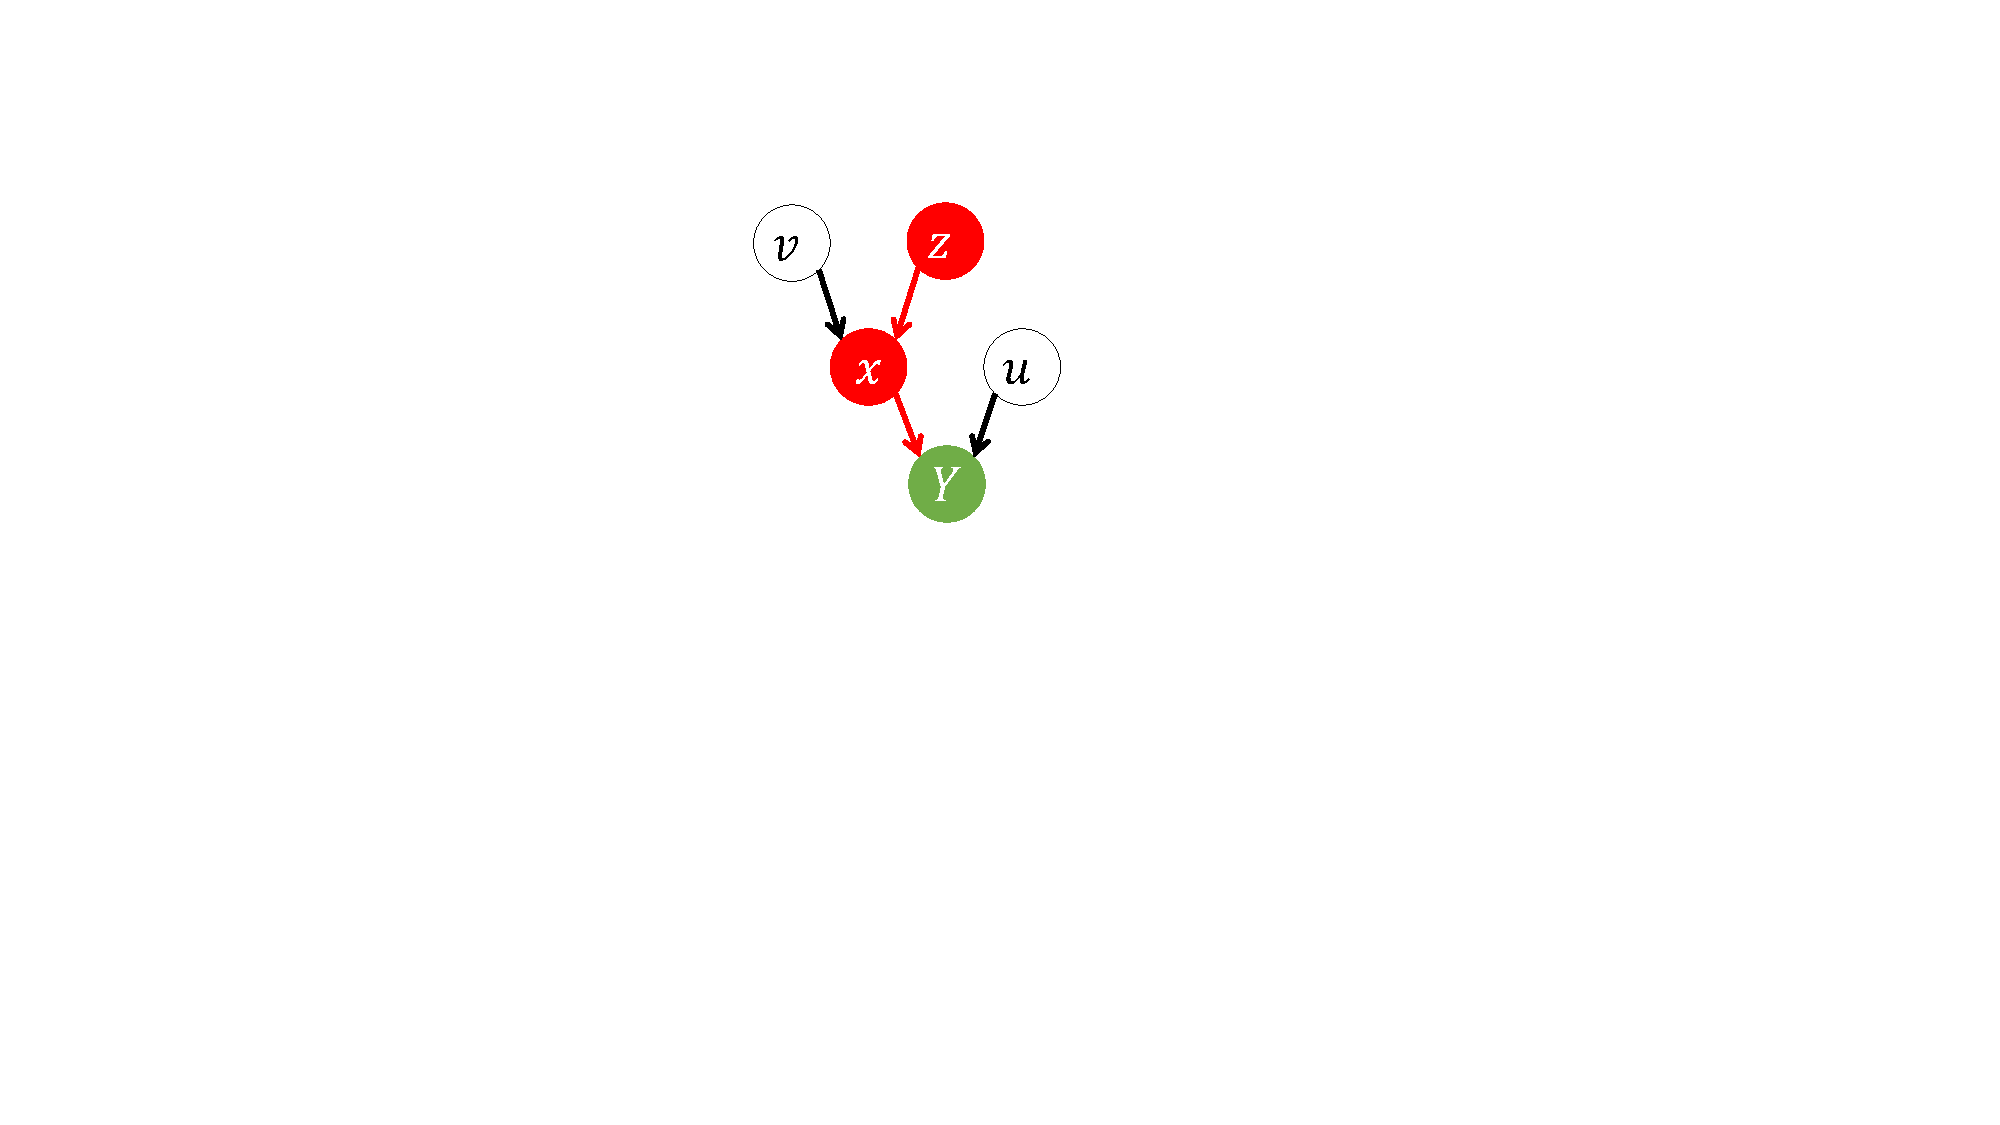
\includegraphics[width=0.2\paperwidth]{example_dag.pdf}
  %
  \caption{The graphical criteria for a valid instrument}
  %
  \label{fig:example_dag}
  %
\end{figure}
%
\noindent
A useful analog to a graph is a family tree, where family members (variables) are connected by arrows representing parentage (causation). In Figure~\ref{fig:example_dag}, the arrows from $\{\mathbf{z}, \mathbf{v}\}$ to $\mathbf{x}$ mean that $\mathbf{z}$ and $\mathbf{v}$ \emph{directly cause} $\mathbf{y}$, further implying that $\mathrm{corr} \left( \mathbf{z}, \mathbf{x} \right) \neq 0$. Analogously, we say that $\{\mathbf{z}, \mathbf{v}\}$ are the \textbf{parents} of $\mathbf{x}$, $\mathbf{x}$ is the \textbf{child} of $\{\mathbf{z}, \mathbf{v}\}$, and $\mathbf{z}$ is a \textbf{spouse} of $\mathbf{v}$. In Figure~\ref{fig:example_dag}, $\mathbf{v}$ directly causes $\mathbf{x}$ and, hence, \emph{indirectly causes} $\mathbf{y}$. The variables that directly or indirectly cause $\mathbf{y}$ are the \textbf{ancestors} of $\mathbf{y}$. Hence, $\mathbf{y}$ and $\mathbf{x}$ are the \textbf{descendants} of $\mathbf{z}$. Lastly, two variables are \textbf{siblings} if they share the same parents.\footnote{See \citet[Section 2.2]{koller2009probabilistic} for further detail on the terminology.}

%#DONE:  stress that Examples 1-3 are there to explain the usefulness of graph learning as well as to illustrate common issues that arise in causality inference

In statistics and biostatistics, causal inference is typically conducted in two stages. The first stage is to estimate the causal structure of the key variable $\mathbf{y}$ (e.g., finding all the parents, children, and spouses of $\mathbf{y}$). The second stage is to estimate the size of the causal effects to or from $\mathbf{y}$. Graph learning is useful because it provides clarity on the causal structure. Moreover, using the following examples, we illustrate that graph learning is critical for causal inference in the sense that failure to learn an accurate graph may result in estimation bias and the related problems of endogeneity, multicollinearity, and misinterpretation.

Field knowledge and experience are often used to construct causal structures in empirical research. But if field knowledge is incomplete, vague, or incorrect, it may compromise any causal inference. Example 1 shows that causal inference relies on the correct temporal ordering of variables, i.e., when the values of variables are determined.
\medskip

\noindent
\textbf{Example 1.} In theoretical and empirical linear regression analysis, $\mathbf{x}$---the parent of $\mathbf{y}$---is typically on the right-hand side of the equation and $\mathbf{y}$ is on the left. This specification is consistent with the temporal ordering: ancestor(s) on the right, descendants on the left. The specification also reflects the fact that a parent $\mathbf{x}$ must be generated before a child $\mathbf{y}$ in the data generating process.

However, field knowledge may fail to indicate the temporal ordering of variables. For example, suppose the true causal structure appears as in Figure~\ref{fig:example_1},

\begin{figure}[H]
%
  \centering
  %
  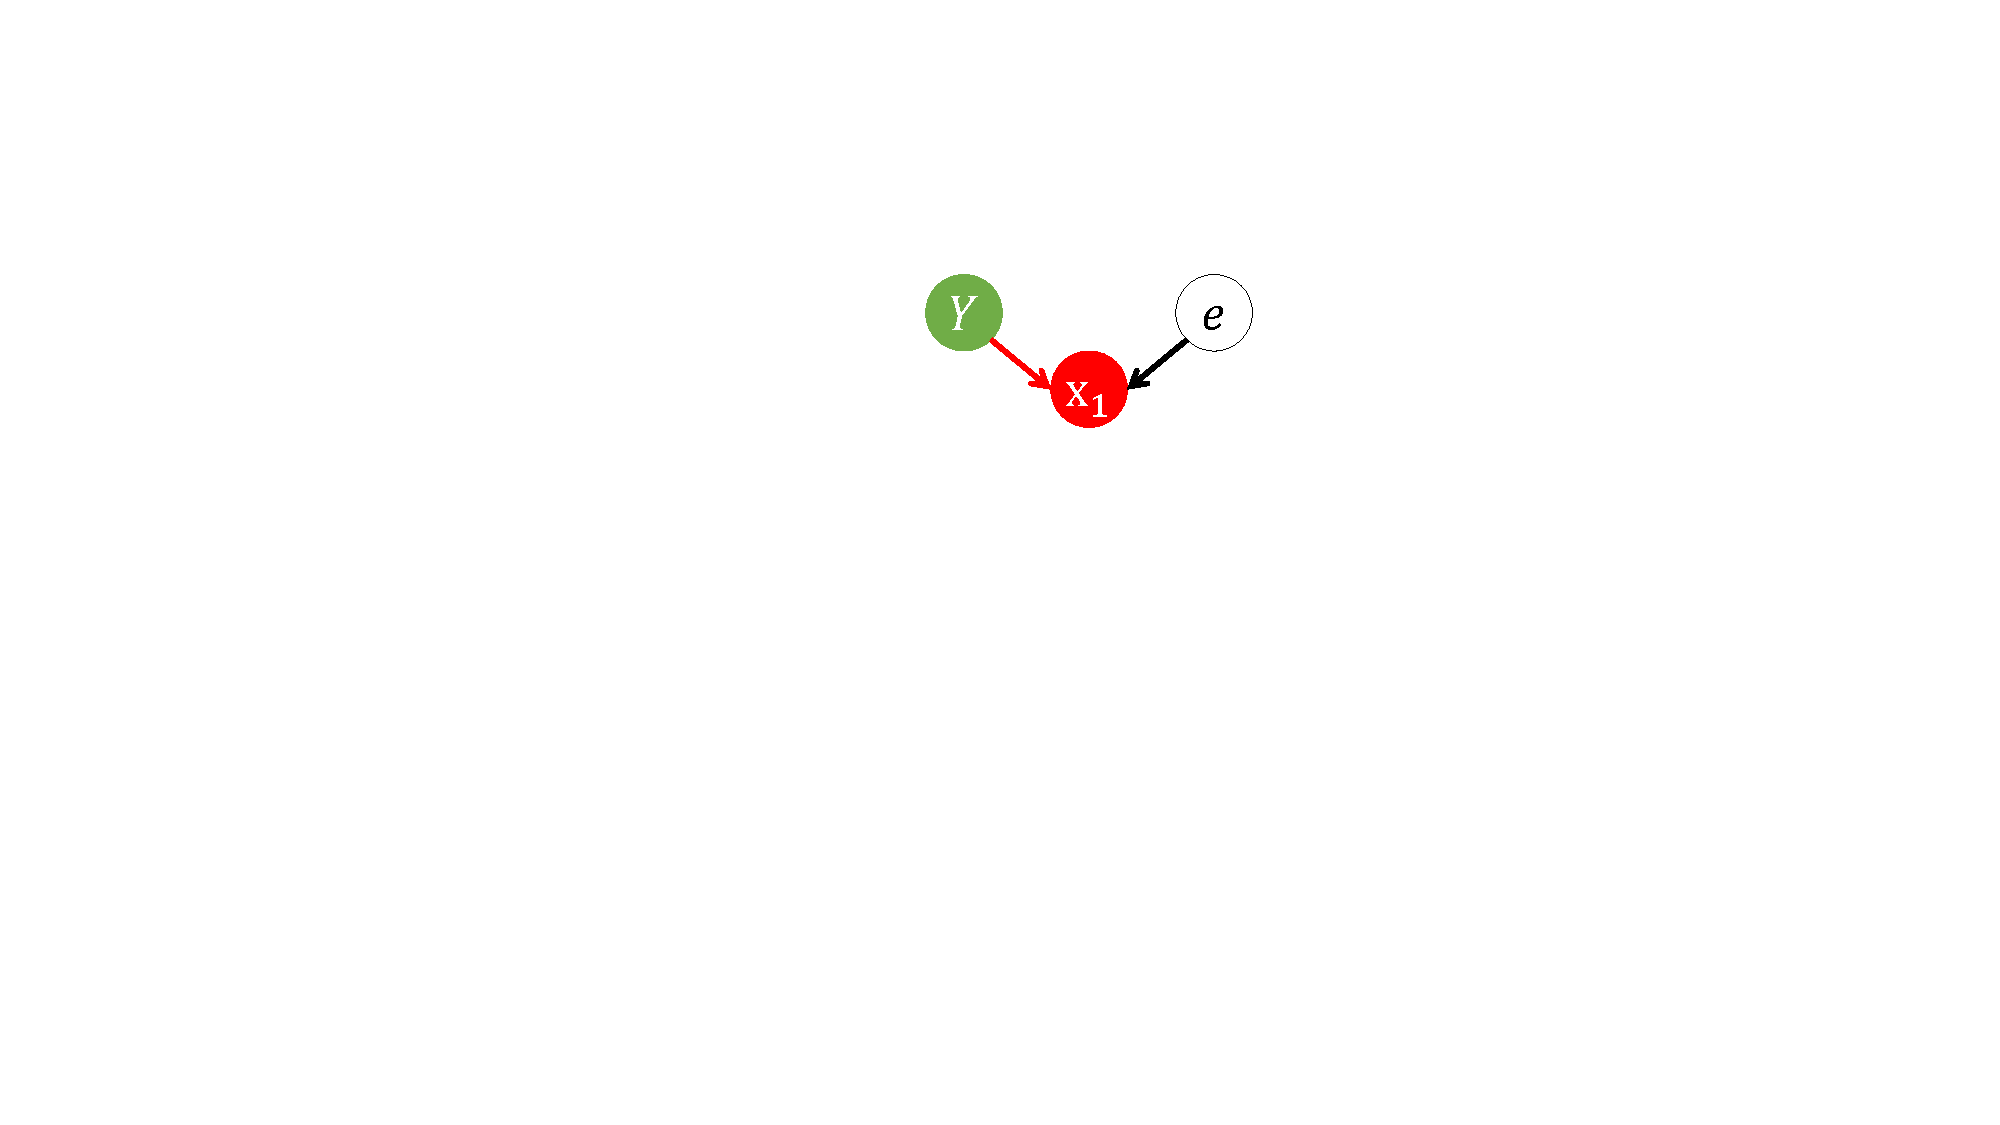
\includegraphics[width=0.2\paperwidth]{Example1_pg.pdf}
  %
  \caption{Example~1 dependence structure.}
  %
  \label{fig:example_1}
%
\end{figure}
%
\noindent
reflecting the data-generating process
%
\begin{equation}
  %
    \mathbf{x}_1 = \beta_0 + \beta_1 \mathbf{y} + e,
  %
  \label{eqn:example_1x}
  %
\end{equation}
%
where both $\mathbf{y}$ and $e$ cause $\mathbf{x}_1$ and $\mathbf{y}$ is independent from $e$. Clearly, (\ref{eqn:example_1x}) implies that, in order to determine the value of $\mathbf{x}_1$, its parents $\mathbf{y}$ and $e$ must be determined first. Suppose that field knowledge holds that $\mathbf{y}$ and $\mathbf{x}_1$ are causally related but is not clear on which is generated first. Because $\mathbf{y}$ is the focus of interest, it will typically be chosen to be the response variable. Hence, the empirical model is
%
\begin{equation}
  %
    \mathbf{y} = \alpha_0 +  \alpha_1 \mathbf{x}_1 + u
  %
  \label{eqn:example_1Y}
  %
\end{equation}
%
with $\alpha_0 = - \beta_0/\beta_1$, $\alpha_1 = 1/\beta_1$ and $u = - e/\beta_1$. Thus, $\mathrm{corr} \left( u, \mathbf{x}_1 \right) = \mathrm{corr} \left( - e/\beta_1, \mathbf{x}_1 \right) \neq 0$ and (\ref{eqn:example_1Y}) suffers from endogeneity. Worse, by mistaking the parent ($\mathbf{y}$) to be a child, the causal structure in (\ref{eqn:example_1Y}) is completely wrong. In this case, it would be difficult to find an instrument to solve the problem: either the model is set up in the correct temporal order, or it will be contaminated by endogeneity; there is hardly any middle ground. $\qed$
\medskip

Example 1 illustrates the importance of specifying the correct parent-child relation in a graph. \textcolor[rgb]{0.00,0.00,1.00}{Such a problem is referred to as \textbf{Markov equivalence} in graph learning, which will be discussed in detail below.} While information criteria and tests can be used to verify whether there is likely to be a non-zero population correlation between $\mathbf{x}$ and $\mathbf{y}$, without further information, they cannot identify whether $\mathbf{x}$ causes $\mathbf{y}$ (or vice versa). To avoid misspecification, one method is to collect the `time stamp' of each variable (i.e., precisely when its value is determined) and order variables chronologically. However, inaccurate chronological ordering is only one of the possible causes of inaccurate causal structure estimation. In Example 2, we show that, without an accurate graph, misdirected causal inference may never return the true result.
\medskip

\noindent
\textbf{Example 2.} In regression, it is well-known that coefficient estimates will be biased and inconsistent if an important covariate is omitted. To avoid omitted variable bias, it is often recommended (e.g., \citet{pratt1988interpretation}) to enlarge the set of potential variables. In this example, we demonstrate that this guidance may cause problems with causal inference.

Suppose that the data are generated by the causal structure in Figure~\ref{fig:example_dag}, that the data generating process follows (\ref{eqn:example_1x}), and that we are interested in the causal effect from $\mathbf{z}$ to $\mathbf{y}$. To avoid omitted variable bias, we include $\mathbf{x}$ in the following regression equation:
%
\begin{equation}
  %
  \mathbf{y} = b_0 +  b_1 \mathbf{x} +  b_2 \mathbf{z} + e,
  %
  \label{eqn:example_2}
  %
\end{equation}
%
As shown in Figure~\ref{fig:example_dag}, $\mathbf{z} \rightarrow \mathbf{x} \rightarrow Y$, implying an indirect causal relationship from $\mathbf{z}$ to $\mathbf{y}$ via $\mathbf{x}$. However, because $\mathbf{x}$ is in the regression, it is removed from the effect of $\mathbf{z}$ on $\mathbf{y}$. Thus, $\mathbf{z}$ is not able to affect $\mathbf{x}$ and, hence, it cannot affect $\mathbf{y}$. As a result, $\mathbf{z}$ will likely not be significant in the regression and we may wrongly conclude that $\mathbf{z}$ has no causal effect on $\mathbf{y}$.

Worse, in empirical analysis, the chosen culprit will likely be multicollinearity rather than an error in causal structure. Noticing the high correlation between $\mathbf{x}$ and $\mathbf{z}$, attention may turn to an omitted confounder for $\mathbf{x}$ and $\mathbf{z}$, resulting in an even larger control variable set. Alternatively, focus may be directed to improving the robustness of the regression, such as by increasing the sample size or regression with robust standard errors. But the source of the problem here is  not multicollinearity, it is including a control a variable that is not relevant. In this case, the only way for single-equation OLS correctly to measure the size of the causal effect of $\mathbf{z}$ on $\mathbf{y}$ is to remove $\mathbf{x}$ from the estimated equation.$\qed$
\medskip

Example~2 illustrates that redundant variables may be just as severe a problem for the causal inference as variable omission. Put another way, too many variables are as problematic as too few. To avoid omitted variable bias, researchers typically focus on enlarging the set of control variables. But this is meaningful only if the correct causal structure is known in advance. Thus, careful selection of variables is necessary before measuring causal effects in OLS. Moreover, different sets of control variables are required under different scenarios. If interest is focussed on the direct (causal) effect to $\mathbf{y}$ (as in Example~2), it is only necessary to include $\mathbf{y}$'s parents. By contrast, if the aim is to measure the indirect effect of $\mathbf{y}$'s grandparents, the parents of $\mathbf{y}$ must be dropped from the regression. Overall, accurate graphs are recommended for causal inference.

Given variable selection is pivotal, careful use of any variable selection algorithm is clearly required. Using the popular lasso algorithm, Example~3 demonstrates the difficulty of correctly identifying the parents of $\mathbf{y}$ in the presence of a strong confounding effect In particular, we show how difficulty with parent identification causes problems with causal structure estimation. To be concise, we follow \citet{zhaoyu06, tibshirani2012strong} and quantify the difficulty of correctly identifying parents with the well-known irrepresentable condition (IRC).

\begin{figure}[H]
  %
  \centering
  %
  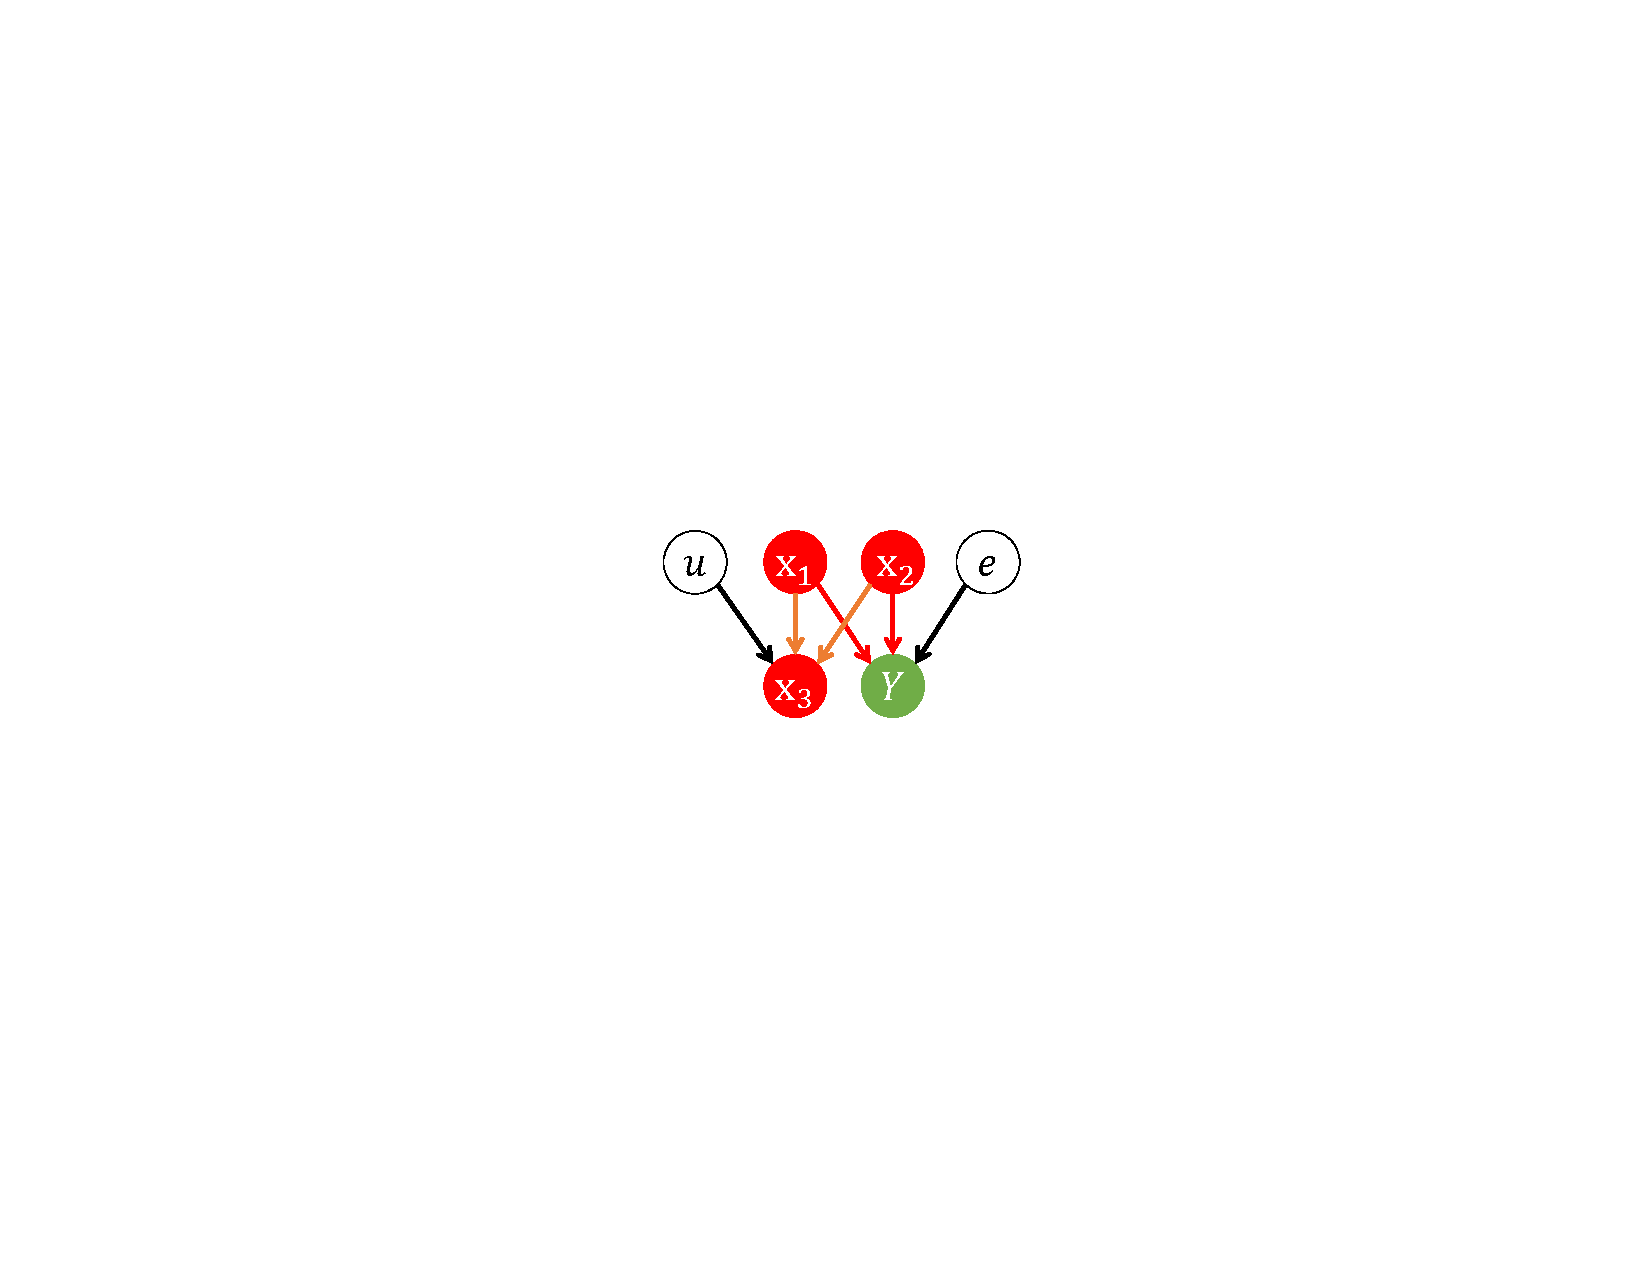
\includegraphics[width=0.35\paperwidth]{Example2_pg.pdf}
  %
  \caption{Example~3 causal structure.}
  %
  \label{fig:example_2}
%
\end{figure}

\noindent
\textbf{Example 3.}\citep{zhaoyu06} Assume the data-generating process is
%
\begin{equation}
  %
  \begin{cases}
  %
    \mathbf{x}_3 = \omega_1 \mathbf{x}_1 + \omega_2 \mathbf{x}_2 + \sqrt{1 - \omega_1^2 - \omega_2^2} \; u, \\
    %
    Y = \beta_1 \mathbf{x}_1 +  \beta_2 \mathbf{x}_2 + \sqrt{1 - \beta_1^2 - \beta_2^2} \; e, \\
    %
  \end{cases}
  %
  \label{eqn:example_3}
  %
\end{equation}
%
where all variables are Gaussian; $\mathbf{x}_1$, $\mathbf{x}_2$, $\mathbf{x}_3$, $\mathbf{y}$, $e$ and $u$ are standardized; $u$ and $e$ are independent from $\left\{u, e\right\}$. Figure~\ref{fig:example_2} shows that $\left\{\mathbf{x}_1, \mathbf{x}_2\right\}$ are the common parents of $\left\{\mathbf{x}_3, Y\right\}$, which are siblings. In this example, we use lasso to find the parents of $\mathbf{y}$.

The IRC states that, $\sum_i \left\vert \omega_i \right\vert < 1$ for variable selection accuracy with lasso (in this case, selecting $\left\{\mathbf{x}_1, \mathbf{x}_2\right\}$ and dropping $\mathbf{x}_3$). Otherwise, with a large probability, lasso-type estimators will take the sibling of $\mathbf{y}$ to be a parent (see the last simulation in \citet{ning2019solar} for detail). Worse, if a group of variables are highly correlated with one another, \citet{zou2005regularization} shows that lasso may randomly drop variables from the group (referred to as the \textbf{grouping effect}), making the selection process extremely sensitive to sampling randomness. In this setting, lasso may wrongly include the sibling $\mathbf{x}_3$ as a parent or dump the true parents $\mathbf{x}_1$ and $\mathbf{x}_2$.

The consequences of incorrect selection extend well beyond variable redundancy in regression. There will be carried-on errors that can render the entire structure misspecified. In Example~3, if the algorithm mistakes the sibling of $\mathbf{y}$ to be its parent, the true nephews of $\mathbf{y}$ will be mistaken as $\mathbf{y}$'s siblings. If the variable selection algorithm mistakes a parent of $\mathbf{y}$ (say $\mathbf{x}_1$) to be redundant, all the true ancestors of $\mathbf{y}$ and the variables indirectly causing $\mathbf{y}$ will also be mistaken as redundant.

The ultimate consequence of a misspecified causal structure is that subsequent statistical decisions regarding $\mathbf{y}$---such as selecting instruments, causal inference, prediction, and forecasting---will be biased. A misspecified causal structure also leads to difficulties with model interpretation and understanding. $\qed$ \medskip

Example~3 suggests a need to confront problems with the lasso estimator in empirical applications with severe multicollinearity or complicated causal structures. To improve variable selection accuracy and robustness, we apply the novel subsample-ordered least-angle regression algorithm (\textbf{solar}) from \citet{ning2019solar}. Solar, which is derived from least-angle regression \citep{efronall04}, significantly outperforms lasso in terms of sparsity and variable-selection accuracy on data with severe multicollinearity and complicated causal structures. In particular, \citet{ning2019solar} shows that, unlike lasso, solar maintains variable selection robustness when IRC fails.

In summary, the three examples show that causal inference requires data with variable time stamps, accurate underlying causal structures, and robust variable selection that tolerates the high dimensionality and multicollinearity caused by complicated causal structures. In this paper,  we address these requirements to arrive at a data-driven method to select and validate instrumental variables in high-dimensional data.

\subsection{Main results}

In this paper we combine two well-known tools from machine learning and biostatistics---variable selection algorithms and graph learning---and apply them to estimate the causal structure of the housing market and the follow-up socio-economic effects using data for 2010 from Sydney, Australia.

The ultrahigh dimensional database consists of school quality data, GIS information, census data, house characteristics, census, and other socio-economic records. We show it is possible to perform a data-driven instrument selection efficiently while purging invalid instruments. The estimated graph of the causal structure of the housing market provides an intuitive interpretation and is consistent with the facts of the Sydney house market, economic theory, and previous empirical findings on house pricing. The estimated graph also returns an accurate and sparse house price model, outperforming other methods in terms of the bias-variance trade-off.

The estimated graph visually depicts the causal structure of house pricing dynamics. Using the graph, we detect endogeneity in house prices, which is confirmed by simultaneous equations modelling. The graph estimation method therefore represents a data-driven, as opposed to ad hoc, approach to detecting endogeneity. Furthermore, we are able to use the graph effectively and efficiently for instrument selection and validation, as confirmed by traditional instrument tests from Durbin, Wooldridge, and Hausman. Moreover, using the graph-recommended instrument, we resolve endogeneity bias in the house price regression, as confirmed by two-stage least squares. Last but not least, the graph estimation method also helps to identify a weak instrument, which is consistent with economic intuition.

The paper is organized as follows. In section~\ref{section:intro}, we introduce variable and instrument selection from the perspective of the random graph. In section~\ref{section:estimation}, we introduce the 2010 Sydney house data and demonstrate in detail the variable selection and graph estimation procedures using the data. In section~\ref{section:application}, we use the estimation results for endogeneity detection and instrument selection. We also show that the graph-based results are consistent with received empirical knowledge on the housing market.

%%%%%%%%%%%%%%%%%%%%%%%%%%%%%%%%%%%%%%%
%%%%%%%%%%%% House data %%%%%%%%%%%%%%%
%%%%%%%%%%%%%%%%%%%%%%%%%%%%%%%%%%%%%%%

\section{Graph and instrument variable selection\label{section:intro}}

Before applying graphs to instrument selection and causal inference, we formally introduce graphs and the graphical definition of instrumental variables. Graph learning terminologies are defined differently across different areas. To be consistent with the literature in machine learning, the following is based on \citet{spirtes2000causation}, \citet{pearl2009causality}, and \citet{koller2009probabilistic}.

\subsection{Graphical criteria for instrument variables}

To properly define an instrumental variable using graphs, we first define how a change in one variable can affect another in a graph. This is represented by the concept of a \textbf{trail}.\footnote{Also referred to as a `path' in some graph learning literature.}

\begin{definition}[Trail of a graph]
  %
  \label{def:trail}
  %
\end{definition}
%
\begin{itemize}
  %
  \item a pair of variables $\left( \mathbf{x}_i, \mathbf{x}_j \right)$ in a graph are \textbf{connected} ($\mathbf{x}_i \rightleftharpoons \mathbf{x}_j$) if either $\mathbf{x}_i \rightarrow \mathbf{x}_j$ or $\mathbf{x}_j \rightarrow \mathbf{x}_i$ ($\mathbf{x}_i$ and $\mathbf{x}_j$ have a parent-child relation).
  %
  \item variables $\mathbf{x}_1, \ldots, \mathbf{x}_k$ in a graph form a \textbf{trail} if, $\forall\, 1 \leqslant i \leqslant k-1$, $\mathbf{x}_i \rightleftharpoons \mathbf{x}_{i+1}$.
  %
\end{itemize}

Intuitively, a trail is a series of variables that are sequentially connected by arrows. A change in $\mathbf{x}_1$ can affect $\mathbf{x}_k$ only if there is a trail between the two variables. From the perspective of joint distribution, if there exists a trail between $\mathbf{u}$ and $\mathbf{v}$, either the unconditional or some conditional correlation between $\mathbf{u}$ and $\mathbf{v}$ is non-zero in population. In Figure~\ref{fig:example_dag}, for example, $\mathbf{z} \rightarrow \mathbf{x} \rightarrow \mathbf{y}$ is a trail, meaning a change in $\mathbf{z}$ can be passed to $\mathbf{y}$ if $\mathbf{x}$ is not conditioned on. Equivalently, the correlation between $\mathbf{z}$ and $\mathbf{y}$ is non-zero if  $\mathbf{x}$ is not conditioned on. In Figure~\ref{fig:example_dag} and (\ref{eqn:instrument}), $\mathbf{z} \rightarrow \mathbf{x} \rightarrow \mathbf{y} \leftarrow \mathbf{u}$ is also a trail, meaning a change in $\mathbf{z}$ can pass to $\mathbf{u}$ only if $\mathbf{y}$ is held constant and $\mathbf{x}$ is not fixed. From the perspective of correlation, $\mathbf{z}$ and $u$ are correlated when $\mathbf{y}$ is held constant and $\mathbf{x}$ is not.

In the examples above, $\mathbf{x}$ plays a key role in the trails. If $\mathbf{x}$ is held constant, the population correlation between $\mathbf{y}$ and $\mathbf{z}$ will be zero. As a result, any change in a variable at one end of the trail cannot affect the variable on the other end. This corresponds to the mistake in Example~2. To describe the role of variables like $\mathbf{x}$, we say that variables at either end of the trail are \textbf{d-separated} by $\mathbf{x}$.\footnote{Also referred to as \textbf{blocked} by $\mathbf{x}$ in some graph learning literature.}

\begin{definition}[d-separation]
  %
  \label{def:d_separation}
  %
  Let $P$ be a trail from the variable $u$ to the variable $v$. Define $u$ and $v$ to be \textbf{d-separated} by a set of variables $Z$ (denoted $u \ind v$ by $Z$) if $u$ and $v$ are independent after conditioning on all the variables in $Z$.

  For example, $u \ind v$ by $Z$ in the following cases.
  %
  \begin{itemize}
    %
    \item $P$ contains a \textbf{directed chain} ($u \leftarrow \cdots \leftarrow m \leftarrow \cdots \leftarrow v$ or $u \rightarrow \cdots \rightarrow m \rightarrow \cdots \rightarrow v$) such that the middle variable $m \in Z$;
    %
    \item $P$ contains a \textbf{fork} ($u \leftarrow \cdots \leftarrow m \rightarrow \cdots \rightarrow v$) such that the middle variable $m \in Z$;
    %
    \item $P$ contains a \textbf{collider} ($u \rightarrow \cdots \rightarrow m \leftarrow \cdots \leftarrow v$) such that the middle variable $m \not\in Z$ and no descendant of $m$ is in $Z$.
    %
  \end{itemize}
  %
\end{definition}

\noindent
Two useful remarks for d-separation follow. First, if $A$ directly causes $B$ (i.e., $A \rightarrow B$) with no intermediate variables, $A$ and $B$ will never be independent, regardless of the variable conditioned on (except $A$ and $B$). In this case, we say that \textit{no} variable can d-separate $A$ and $B$ (sometimes denoted $A \not\ind B$). Second, as illustrated in Figure~\ref{fig:graphical_criteria_instrument}, if $A$ and $B$ have no causal relation whatsoever, we say \textit{any} variable (for example, variable $C$) can d-separate $A$ and $B$ (sometimes denoted $A \ind B$).%
\begin{figure}[H]
  %
  \centering
  %
  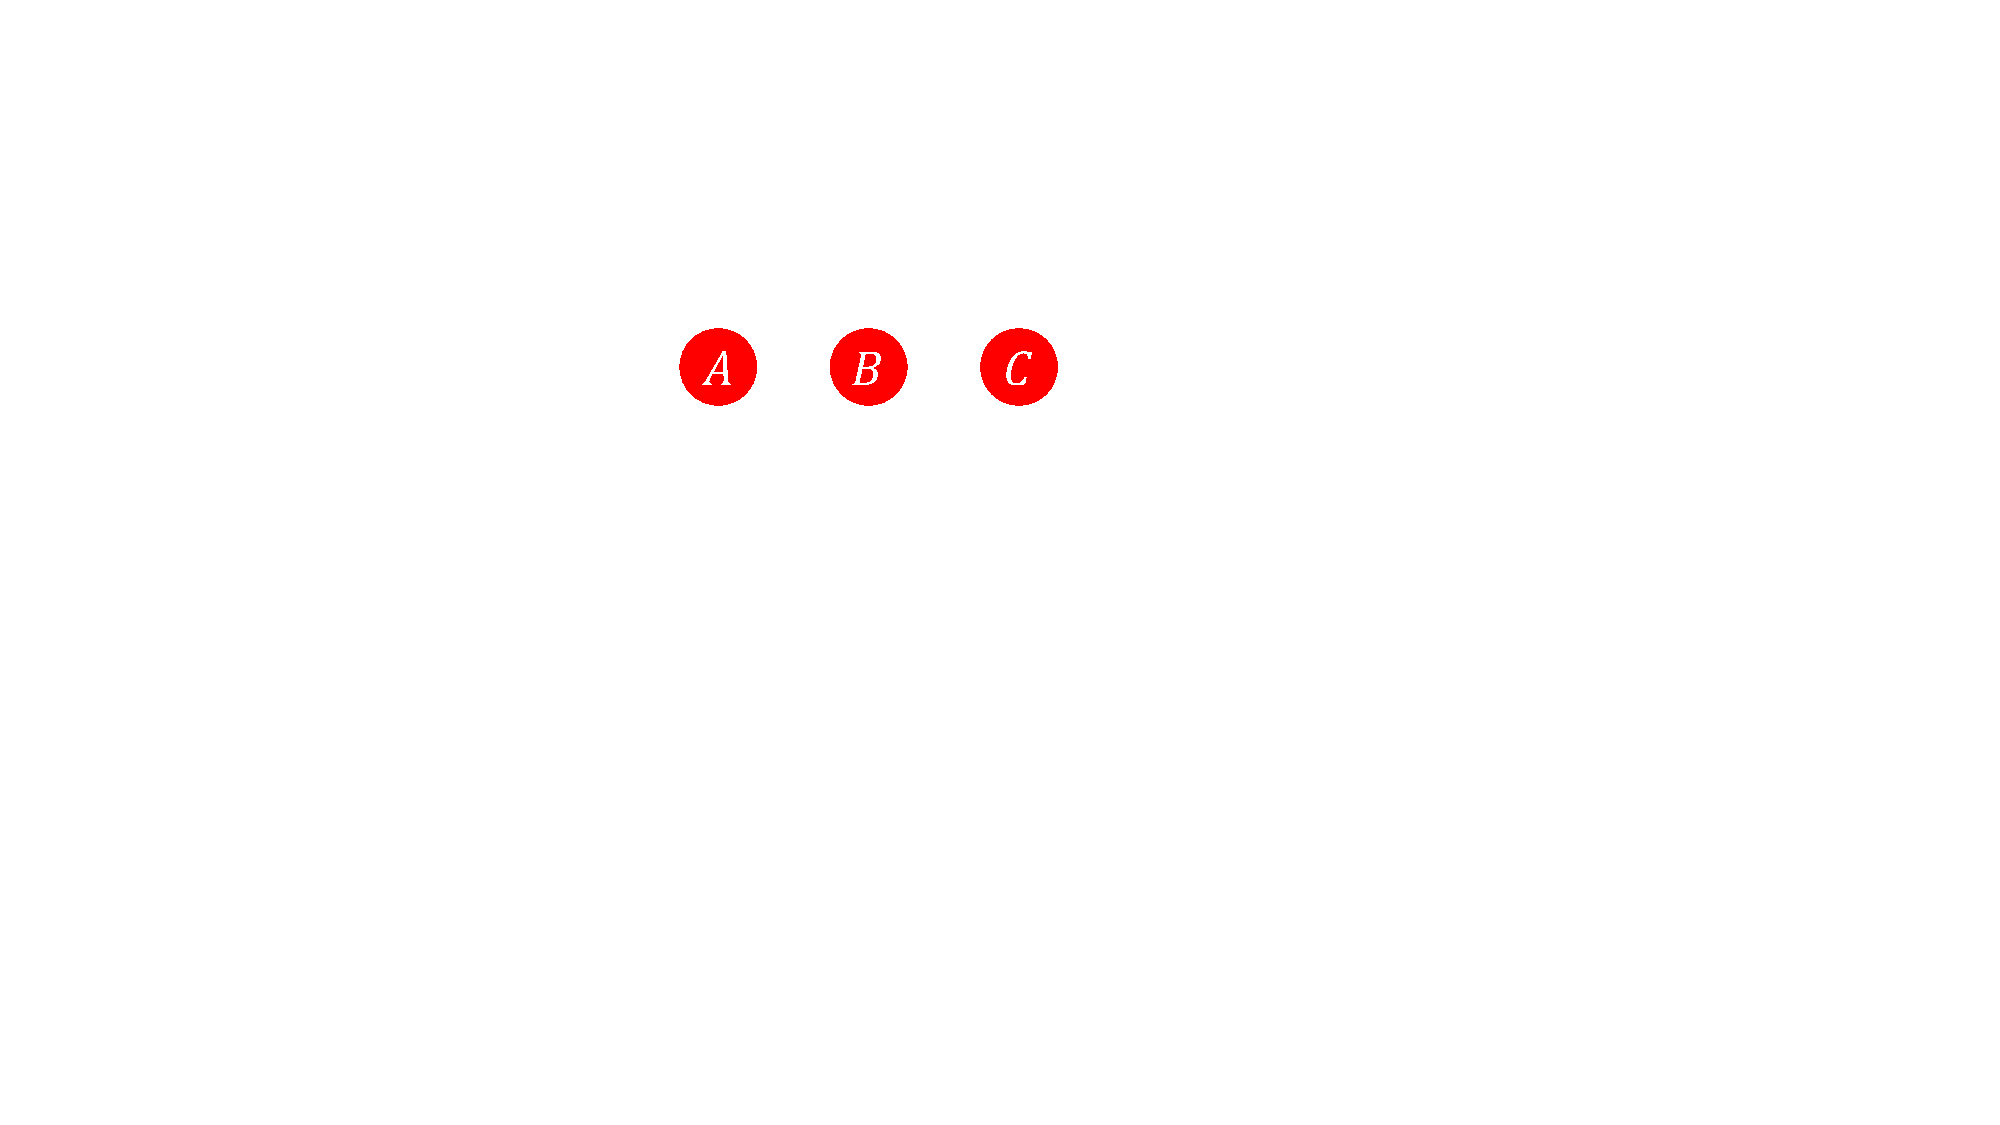
\includegraphics[width=0.2\paperwidth]{graphical_criteria_instrument.pdf}
  %
  \caption{No dependency between $A$, $B$, or $C$.}
  %
  \label{fig:graphical_criteria_instrument}
  %
\end{figure}

Using the concept of d-separation, the graphical definition of an instrument can be precisely defined, following \citet{brito2002generalized}, \citet{pearl2009causality} and \citet{silva2017learning}, and illustrated in Figure~\ref{fig:instrument}.\footnote{As shown by \citet{brito2002generalized} and \citet[pp.~247-248]{pearl2009causality}, the complete set of graphical criteria for an instrument is more complicated than our definition as it incorporates the idea of conditional instruments in a graph. To avoid being sidetracked, we leave further discussion to Appendix~\ref{App:IV_def}.}

\begin{definition}[Graphical criteria for instruments]
  %
  \label{def:instrument_variable}
  %
  Let $\mathbf{x}, \mathbf{z}$ and $\mathbf{y}$ be variables in graph $G$ where $\mathbf{x}$ directly causes $\mathbf{y}$. $\mathbf{z}$ is an instrument for $\mathbf{x}$ if
  %
  \begin{itemize}
    %
    \item[\textbf{G1}] $\mathbf{z}$ and $\mathbf{y}$ can be d-separated by any variable in $G_{\overline{\mathbf{x}}}$, where $G_{\overline{\mathbf{x}}}$ is the graph in which the effect from $\mathbf{x}$ to $\mathbf{y}$ is cut off (sometimes denoted $\left(\mathbf{z} \ind Y \right)_{G_{\overline{\mathbf{x}}}}$).
    %
    \item[\textbf{G2}] $\mathbf{z}$ and $\mathbf{y}$ cannot be d-separated by any variable in $G$ (sometimes denoted $\left(\mathbf{z} \not\ind \mathbf{x} \right)_G$).
    %
  \end{itemize}
  %
\end{definition}

\begin{figure}[h]
  %
  \centering
  %
  \subfloat[\label{fig:instrument1}graph $G$, where $\mathbf{z} \not\ind \mathbf{x}$]
  {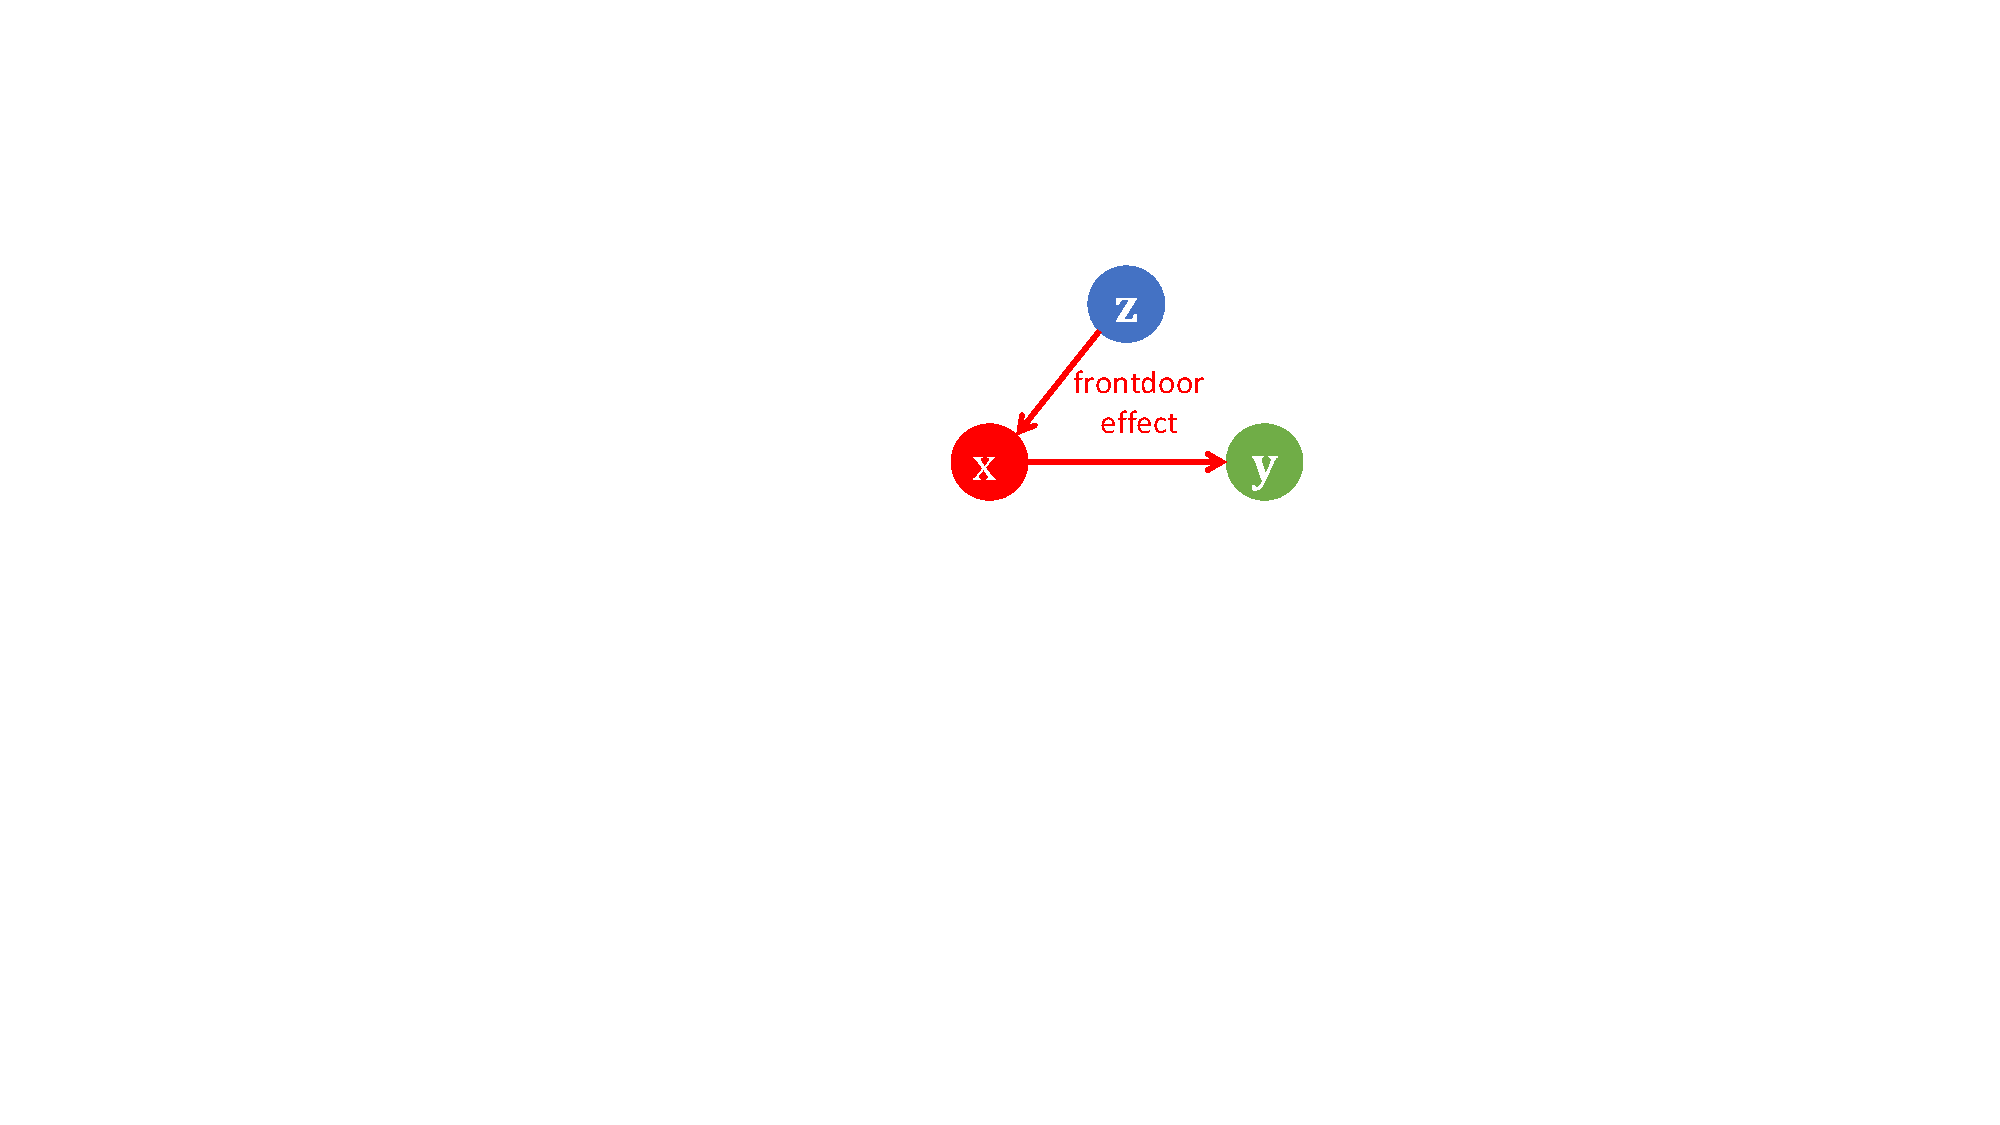
\includegraphics[width=0.2\paperwidth]{instrument1.pdf}}
  \hfil
  \subfloat[\label{fig:instrument2}graph $G_{\overline{X}}$, where $\mathbf{z} \ind Y$]
  {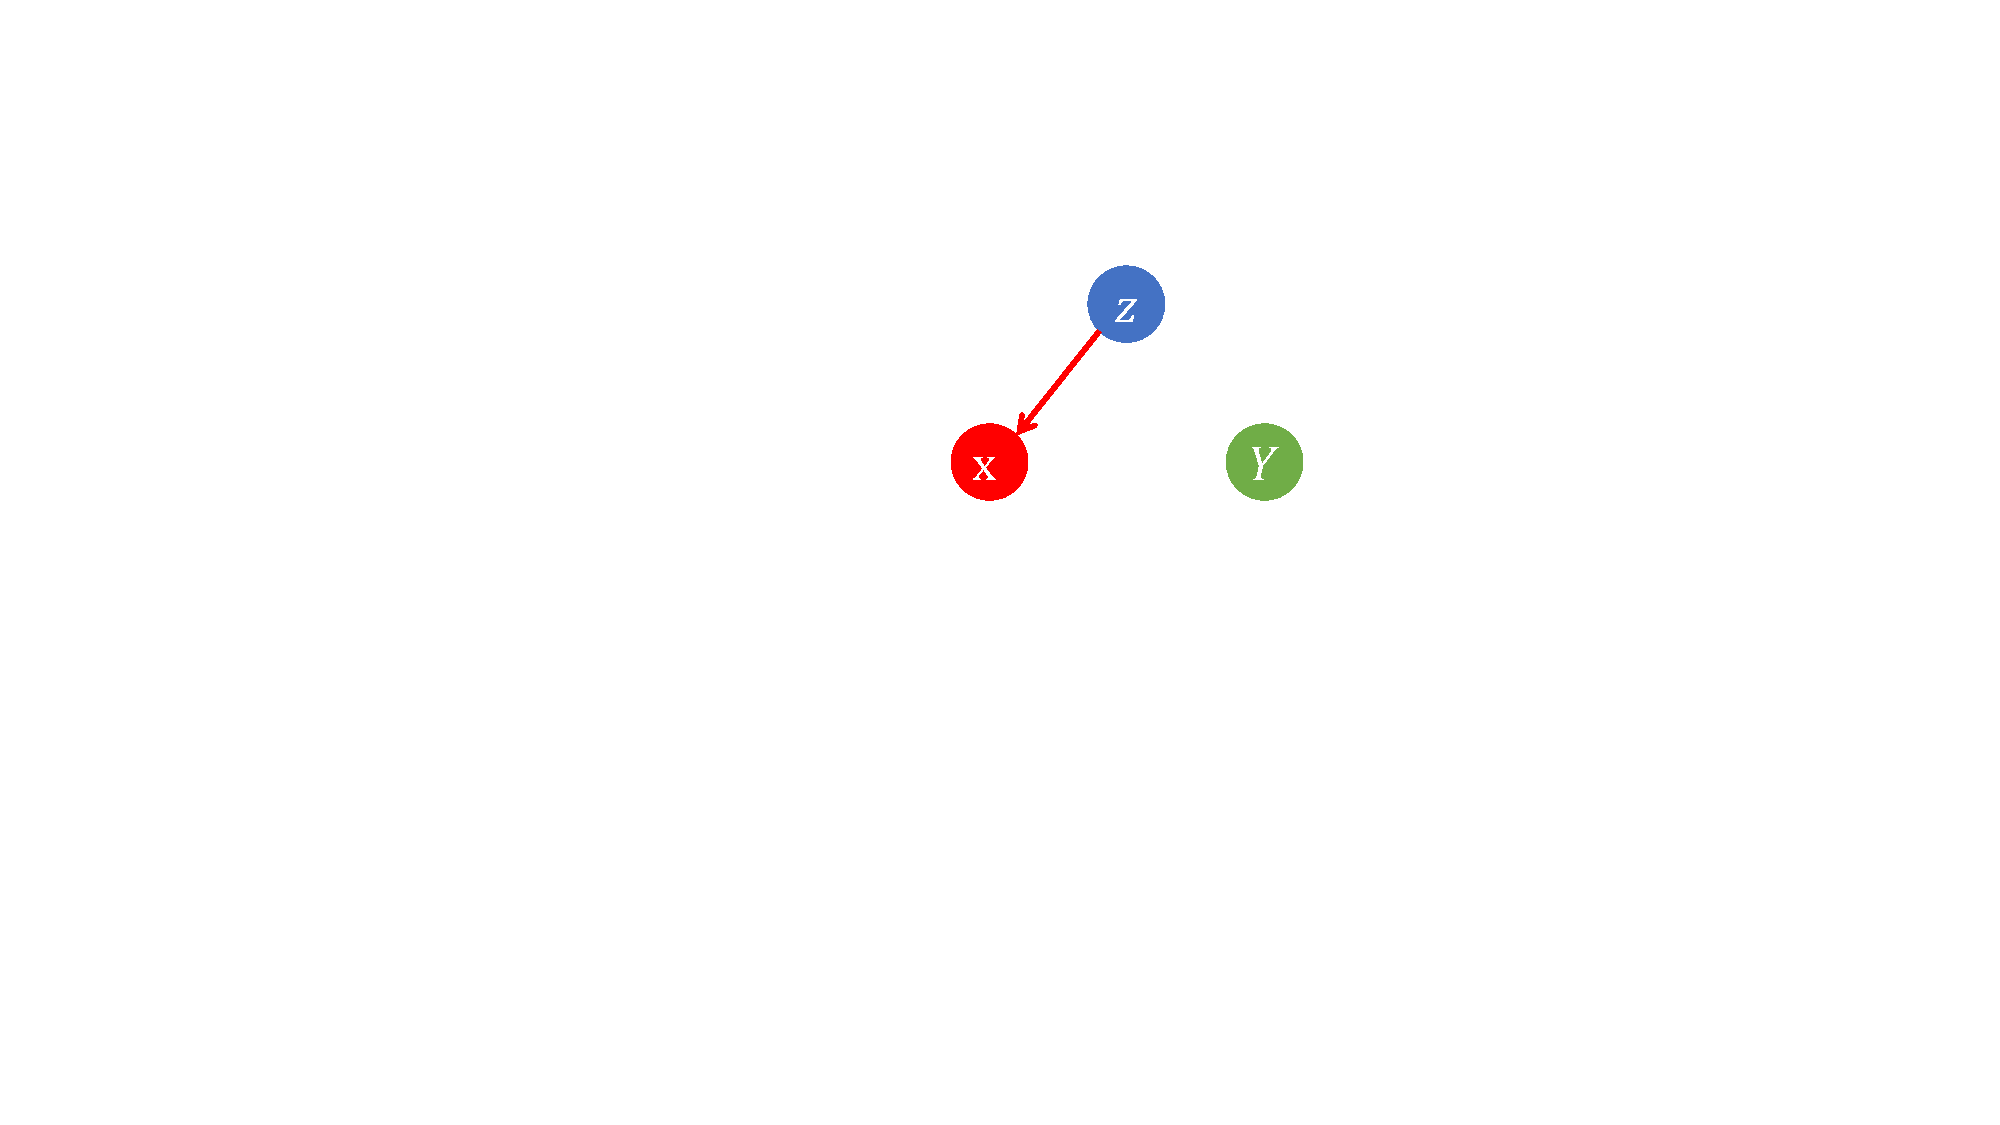
\includegraphics[width=0.2\paperwidth]{instrument2.pdf}}
  %
  \caption{Illustration: definition of an instrumental variable.}
  \label{fig:instrument}
  %
\end{figure}

\noindent
Graphically, G1 means that, if we remove all the causal effects from $\mathbf{x}$ to $\mathbf{y}$, $\mathbf{z}$ cannot affect $\mathbf{y}$ any more.\footnote{Sometimes, G1 is modified to $\left(\mathbf{z} \ind Y \right)_{G_{\overline{\mathbf{x}}}}$, where $G_{\overline{\mathbf{x}}}$ is obtained by removing all the arrows entering $\mathbf{x}$ from the graph $G$, but Definition~~\ref{def:instrument_variable} is the more common definition of instrument. Nonetheless, both versions mean that the effect from $\mathbf{z}$ to $\mathbf{y}$ must go only through $\mathbf{x}$.} Similarly, G2 means that the effect from $\mathbf{z}$ to $\mathbf{x}$ cannot be broken by holding any variable constant. Both G1 and G2 mean that the effect from $\mathbf{z}$ to $\mathbf{y}$ must go only through $\mathbf{x}$. Put another way, holding $\mathbf{x}$ constant, $\mathbf{z}$ cannot affect $\mathbf{y}$ by any means. In graph learning, the effect from $\mathbf{z}$ to $\mathbf{y}$ via the (endogenous) variable $\mathbf{x}$ is also referred to as the frontdoor effect (FE) (Figure~\ref{fig:instrument1}). Moreover, Definition~\ref{def:instrument_variable} is a generalized version of the usual definition of an instrument in regression analysis. Assuming that $\mathbf{x}$ causes $\mathbf{y}$ in (\ref{eqn:instrument}), $\mathrm{corr} \left( \mathbf{z}, \mathbf{x} \right) \neq 0$ implies the existence of a FE. Likewise, $\mathrm{corr} \left( \mathbf{z}, u \right) = 0$ implies there does not exist any effect from $\mathbf{z}$ to $\mathbf{y}$ that does not go through $\mathbf{x}$ (also referred to as no backdoor effect (BE)).\footnote{In other graph learning literature (\citet{pearl2009causality}, for example), this is also referred to as ``$\mathbf{x}$ satistfies the `no backdoor criterion' for the causal effect between $\mathbf{z}$ and $\mathbf{y}$''}

Classical machine learning and biostatistics research [e.g., \citet{spirtes2000causation} and \citet{pearl2009causality}] shows that Definition~\ref{def:instrument_variable} implies the classical definition based on the regression error, referred to as the error-based criteria for instrument variables. For more detailed analysis and examples, see Appendix~\ref{App:IV_def}.

\begin{figure}[H]
	%
	\centering
	%
	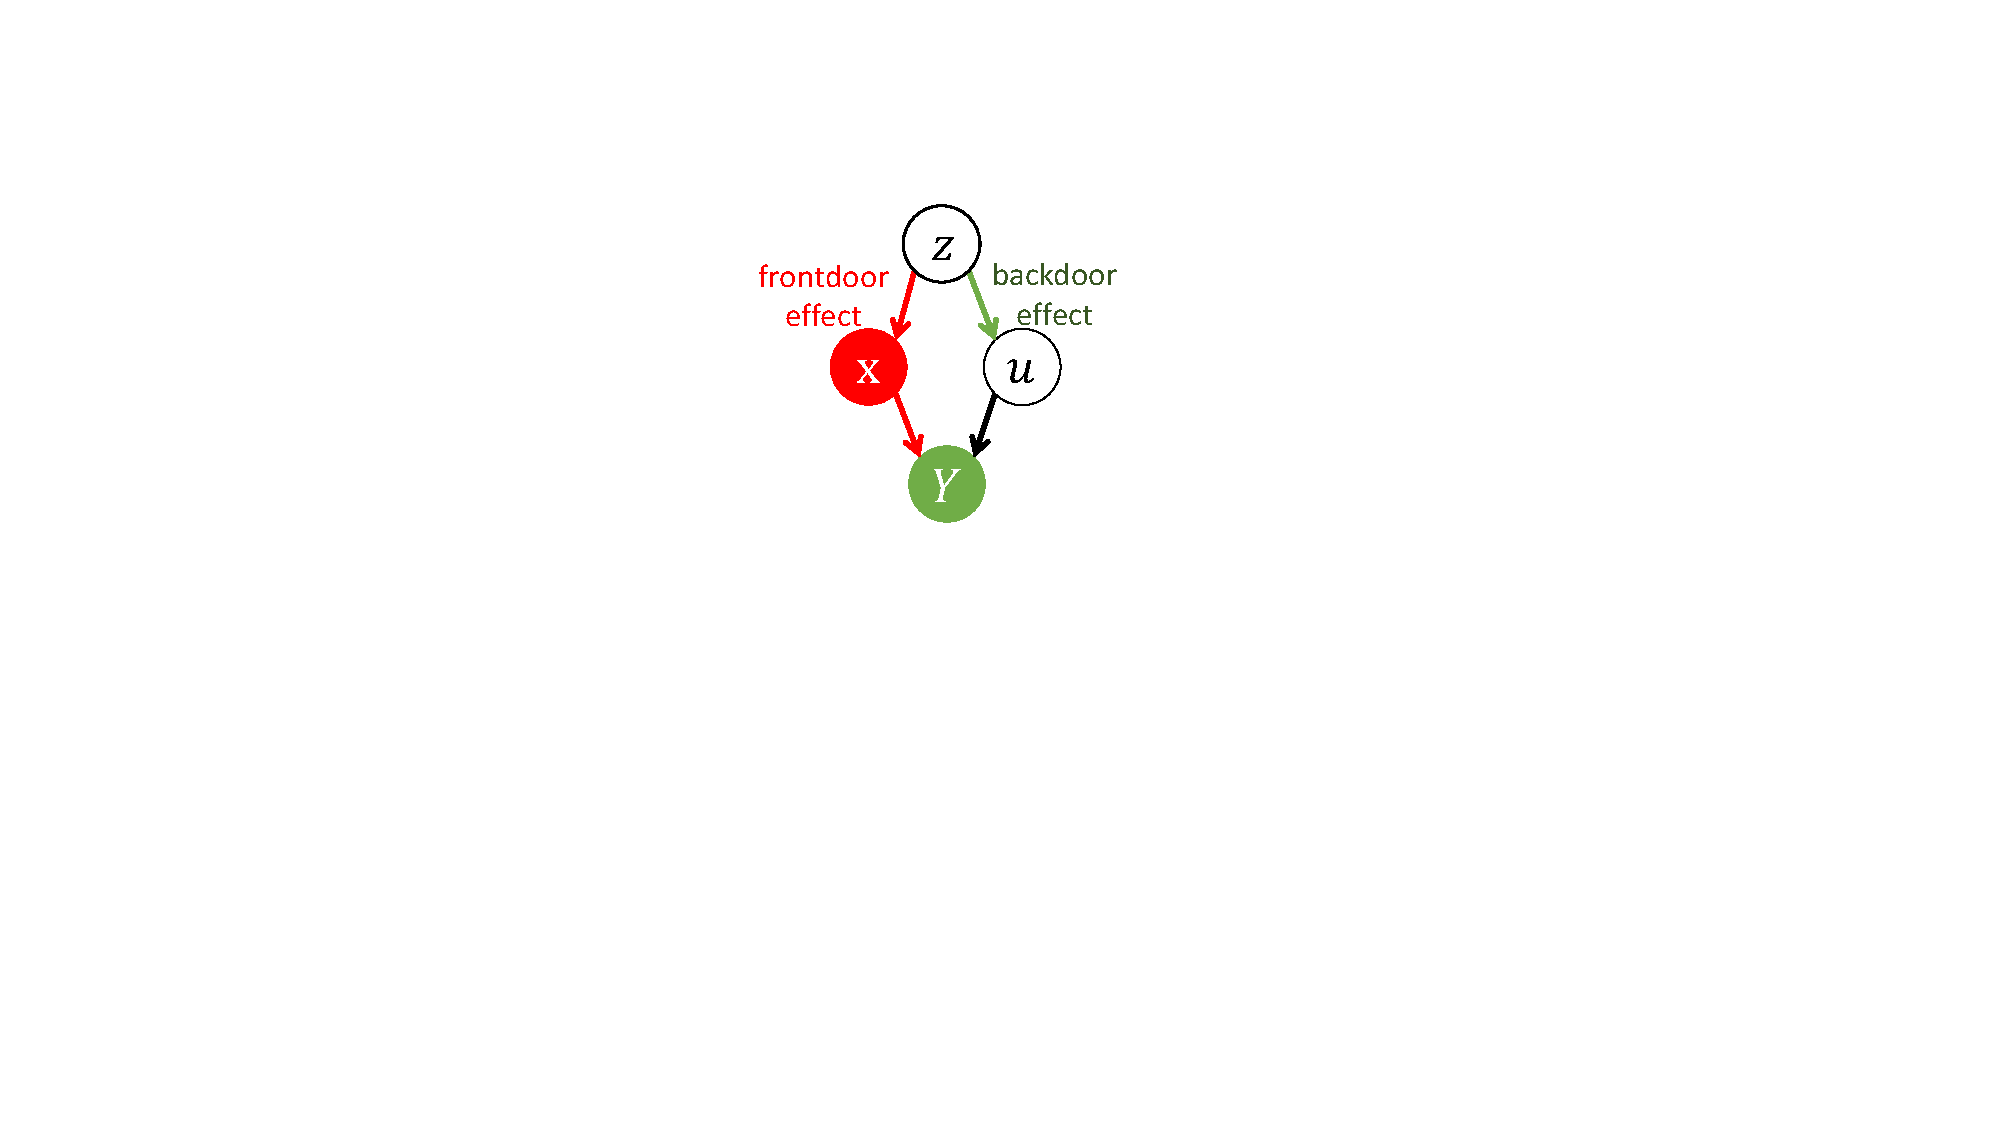
\includegraphics[width=0.15\paperwidth]{not_instrument1.pdf}
	%
	\caption{Illustration: violation of Definition~\ref{def:instrument_variable}.}
	\label{fig:not_instrument1}
	%
\end{figure}

\noindent
As \citet{spirtes2000causation} and \citet{pearl2009causality} show, Definition~\ref{def:instrument_variable} can be used to identify instruments in a graph. Take Figure~\ref{fig:not_instrument1} as an example. A classical case in econometrics, Figure~\ref{fig:not_instrument1} contains an arrow from $\mathbf{z}$ to $u$. As a result, $\mathrm{corr} \left( \mathbf{z}, u \right) \neq 0$ in (\ref{eqn:instrument}), implying $\mathbf{z}$ is not a valid instrument. Equivalently, the arrow from $\mathbf{z}$ to $u$ allows $\mathbf{z}$ to affect $\mathbf{y}$ separately from the endogenous variable $\mathbf{x}$, which is a BE. As a result, Figure~\ref{fig:not_instrument1} violates G1 since $\mathbf{z}$ and $\mathbf{y}$ are not independent even though $\mathbf{x}$ is held constant.

\subsection{Variable selection for graph learning}

Figure~\ref{fig:instrument} and Appendix~\ref{App:IV_def} reveal an advantage of the graphical approach to instrumental variable selection. If we can accurately estimate the graph (or at least estimate the role of each variable relative to $\mathbf{y}$), choosing an appropriate instrumental variable is straightforward. Hence, accurate graph estimation is at the core of data-driven causal inference. As Examples~2 and~3 illustrate, variable omission and variable redundancy can both mislead graph learning and, consequently, causal inference. To avoid variable omission, it is always safe to start graph learning from a dataset that contains as many relevant variables as possible. Unfortunately, minimizing the possibility of variable omission may result in a large number of potential variables in the graph, raising dimensionality and computational issues. Moreover, Examples~2 and~3 show that including redundant variables may lead to misleading and counterintuitive results. Hence, it is necessary to accompany graph learning with variable selection (aka feature selection, variable elimination, etc.).

To build the connection between variable selection and regression-based causal inference, we follow the common linearity assumptions [e.g., \citet{bollen1989structural, geiger1994learning, spirtes2000causation}] as follows:
%
\begin{itemize}
  %
  \item[\textbf{A1}] the data generating process of each variable may be represented by linear regression;
  %
  \item[\textbf{A2}] dependencies among variables may be represented by correlation (e.g., (\ref{eqn:instrument})).
  %
\end{itemize}

\textbf{A1} and \textbf{A2} imply that the causal structure is linear or, equivalently, that there is a linear graph in the population. It is worth noting we do not assume that the linear equation is a perfect representation of the data generating process. In fact, it is quite common that linear models to suffer misspecification, especially when there is uncertainty about the linearity of the data-generating process. Hence, in this paper, we start graph learning from a linear graph and check the appropriateness of the linearity assumption after estimation. If linearity is not appropriate, it is possible to add a nonlinearity pattern (e.g., neural network, kernel regression in reproducing kernel Hilbert spaces) into the graph learning.

With \textbf{A1} and \textbf{A2}, all graphs in this paper are linear graphs and graph learning can be understood from the perspective of high-dimensional regression analysis. In classical regression analysis, significance tests and variable selection algorithms are applied to find variables with non-zero population coefficients. A regression coefficient represents the conditional correlation between the corresponding covariate and the response variable, holding other covariates constant. As a result, variable selection algorithms aim to find variables that are conditionally correlated to $\mathbf{y}$ in the population, holding all other variables constant.\footnote{After standardizing the response variable and all covariates, the regression coefficient of $\mathbf{x}_i$ is the conditional correlation between $\mathbf{x}_i$ and $\mathbf{y}$, holding all other covariates constant.} In graph learning, the set of such variables is called the \textbf{Markov blanket of $\mathbf{y}$}, denoted MB($\mathbf{y}$), which includes the parent(s), children and spouse(s) of $\mathbf{y}$. Hence, in linear graphs, recovering the MB($\mathbf{y}$) is equivalent to finding the true variables in the linear regression of $\mathbf{y}$ on all other variables, illustrated graphically in Figure~\ref{fig:variable_selection} and analysed in Example~4.\footnote{For a more general explanation and examples, see \citet{pearl2009causality}, \citet{koller2009probabilistic}, or \citet{scutari2014bayesian}.}

\begin{figure}[h]
  %
  \centering
  %
  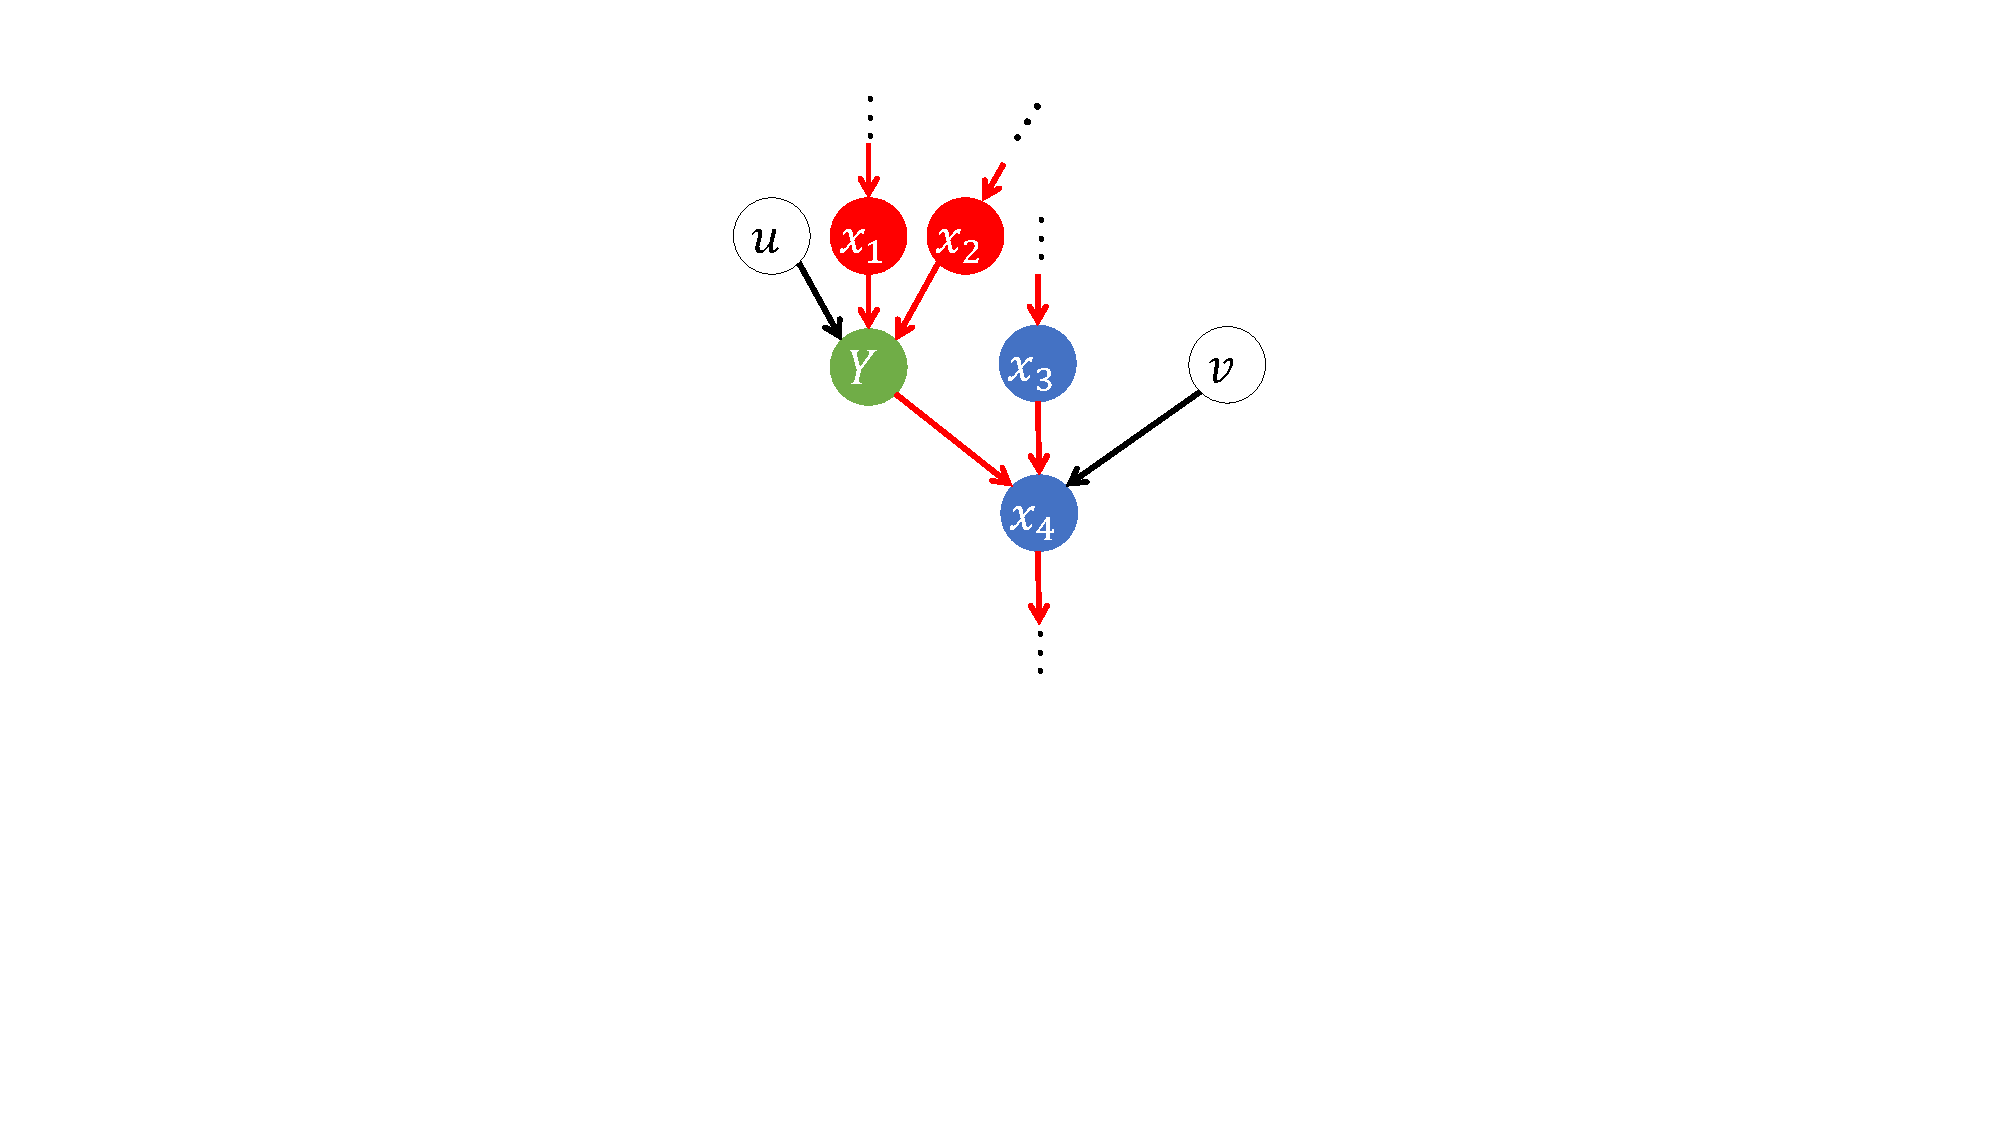
\includegraphics[width=0.3\paperwidth]{variable_selection.pdf}
  %
  \caption{Illustration: recovering the Markov blanket for $\mathbf{y}$.}
  \label{fig:variable_selection}
  %
\end{figure}

\noindent
\textbf{Example 4.} In Figure~\ref{fig:variable_selection}, $\mathbf{u}$ and $\mathbf{v}$ are independent latent noise terms; $\left\{\mathbf{x}_1, \mathbf{x}_2, \mathbf{u}\right\}$ are the parents of $\mathbf{y}$; $\left\{\mathbf{x}_3, \mathbf{v}\right\}$ are spouses of $\mathbf{y}$; and $\left\{\mathbf{y}, \mathbf{x}_3, \mathbf{v}\right\}$ together cause $\mathbf{x}_4$. Together with A1 and A2, the data-generating process in Figure~\ref{fig:variable_selection} is the following linear system,
%
\begin{equation}
  %
  \begin{cases}
    %
    \mathbf{y}   & = \alpha_0 + \alpha_1 \mathbf{x}_1 + \alpha_2 \mathbf{x}_2 + \mathbf{u},\\
    %
    \mathbf{x}_4 & = \beta_0  + \beta_1 \mathbf{y}    + \beta_1 \mathbf{x}_3  + \mathbf{v}.
    %
  \end{cases}
  %
  \label{eqn:variable_selection}
  %
\end{equation}
%
Holding $\left\{\mathbf{x}_1, \mathbf{x}_2\right\}$ constant, (\ref{eqn:variable_selection}) shows that all the variation in $\mathbf{y}$ is caused only by $\mathbf{u}$ (mathematically, $\mathbf{y} \vert \left\{\mathbf{x}_1, \mathbf{x}_2\right\} = \mathbf{u}$). Put another way, after partialing out $\left\{ \mathbf{x}_1, \mathbf{x}_2 \right\}$ from $\mathbf{y}$, the variation in $\mathbf{u}$ can be explained by the children of $\mathbf{y}$. As a result, the independence between $\mathbf{v}$ and $\left\{ \mathbf{x}_1, \mathbf{x}_2 \right\}$ and the second equation of (\ref{eqn:variable_selection}) imply that
%
\begin{align}
  %
  \mathbf{u} = & \mathbf{y} \vert \left\{\mathbf{x}_1, \mathbf{x}_2\right\} \notag \\
    = & - \frac{\beta_0}{\beta_1}  + \frac{1}{\beta_1} \mathbf{x}_4 \vert \left\{\mathbf{x}_1, \mathbf{x}_2\right\} - \frac{\beta_2}{\beta_1} \mathbf{x}_3 \vert \left\{\mathbf{x}_1, \mathbf{x}_2\right\} - \frac{\mathbf{v}}{\beta_1} .
  %
  \label{eqn:variable_selection_example}
  %
\end{align}
%
After replacing $\mathbf{u}$ in (\ref{eqn:variable_selection}) with the right-hand side of (\ref{eqn:variable_selection_example}), the data generating process of $\mathbf{y}$---the first equation in (\ref{eqn:variable_selection})---reduces to the following population regression equation of $\mathbf{y}$ on its MB,
%
\begin{align}
  %
  \mathbf{y} = \gamma_0 + \gamma_1 \mathbf{x}_1 + \gamma_2 \mathbf{x}_2 + \gamma_3 \mathbf{x}_3 + \gamma_4 \mathbf{x}_4 + \mathbf{e},
  %
  \label{eqn:reduced_form_example}
  %
\end{align}
%
%#DONE: explain the endogeneity between e and  children of Y
%
where $\mathbf{e}$ is a linear function of $\mathbf{v}$. Hence, (\ref{eqn:reduced_form_example}) is the population reduced form of the linear system (\ref{eqn:variable_selection}), where only the MB variables are informative (or true).$\qed$

\bigskip
Example~4 implies that if a consistent variable selection algorithm (for example, lasso-type estimators and SCAD) is applied to~(\ref{eqn:reduced_form_example}), it should select only $\left\{ \mathbf{x}_1, \mathbf{x}_2, \mathbf{x}_3, \mathbf{x}_4 \right\}$. \citet{zhaoyu06} show that the IRC almost surely guarantees the variable selection consistency of lasso. Thus, assuming IRC holds, lasso is likely to select only the true variables in~(\ref{eqn:reduced_form_example})---the MB of $\mathbf{y}$---given sufficient data. In other words, variable selection in the regression of $\mathbf{y}$ is equivalent to finding the MB of $\mathbf{y}$ in a linear graph. Having said that, given the complicated causal structure, variables in the graph may be heavily correlated. As a result, when applying lasso-type estimators to linear graphs, it is important to check correlations between selected variables and dropped variables in order to detect potential violation of the IRC.

Score-based and constraint-based learning work combinatorially and require a high computation load. Thus, classical graph learning algorithms do not work well when dimensionality is high. However, by purging redundant variables from the MB, the possible combinations of causal effects to and from $\mathbf{y}$ are reduced exponentially. Thus, accurate MB estimation speeds up graph learning, facilitating causal inference and instrument selection on $\mathbf{y}$.

\section{Graph estimation with Sydney house market data \label{section:estimation}}

In this section, we prepare the Sydney real estate database for graph learning and causal inference. In applied econometrics, house prices are typically represented by linear regression on easily-measured attributes (e.g., the number of bedrooms, bathrooms, land size, distance to amenities, etc.). To avoid variable omission bias, the database includes as much objective information as possible that is relevant to the market value of particular a house, much of which is determined by the location of the property, its unique features, and the characteristics of the neighbourhood. We apply a variable selection algorithm to the `big data' and try to find as many Markov Blanket members of house price as possible.

\subsection{Description and sources of data}

The database is assembled from more than 10 different datasets, including 2010 Sydney house sales transaction and attribute data (including every 2010 sale of a house within roughly 10km south and east of the city centre), 2010 and 2011 Sydney crime data by suburb, 2010 GIS data (extracted and complied from the Sydney geospatial topological database, climate database, pollution database, and Google Maps database), 2011 census data by Statistical Area Level 1 (SA1, the smallest census area in Australia, with an average size of 200 people or 60 households), 2009 local school quality and catchment data, 2010 Sydney traffic data, data on public transport (all routes as well as the location of train stations, ferry wharfs, and bus stops), and so on. To speed up computation and data manipulation, we synthesize all databases using \textsf{Aparche Spark} on Google Cloud. Altogether, the database is over 200GB; there are more than 10,000 variables and roughly 11,000 observations.

The data are collected from many different sources. Some house features are reported in real-estate advertising and others are scraped from Google searches using a \textsf{Python} internet scraper. The distances of each house to nearest key locations are computed in QGIS---a open-source \textsf{Python}-based geographical information system---using the GPS location of each house and geodata collected from Google Maps and Department of Land and Natural Resources, New South Wales. The 2009 Index of Community Socio-Educational Advantage (ICSEA) score---an measure of the socio-educational background of students at each school---is collected from the Australian Curriculum, Assessment and Reporting Authority (ACARA). The variables on local school quality (measured by average National Assessment Program -- Literacy and Numeracy (NAPLAN) examination results) are also collected from ACARA. The 2009 and 2010 geolinked crime data are collected from the Australian Bureau of Statistics and Department of Justice, New South Wales. The 2011 census data, traffic data, climate data, geospatial topological database and pollution database are acquired from the Australian Bureau of Statistics. Socio-economic data are observed by SA1, the smallest census statistical area for which public data are available. To avoid Simpson's paradox, we only incorporate SA1 that only covers houses, ruling out apartments.\footnote{In other graph learning literature, Simpson's paradox is referred to as Simpson's reversal or the reversal paradox. For example, see \citet{simpson1951interpretation} and \citet{blyth1972simpson}.} The detailed variable list is attached in Appendix~2 as a csv file.

\subsection{First stage variable selection}

As explained in above, graph learning and MB selection typically work well on datasets with small $p/n$. However, in our data, $n$ and $p$ are both larger than 10,000. Not only are those values well above the computation limit of graph learning but, given the high dimensionality, there are likely to be many variables that are irrelevant to the house price MB. As a result, following \citet{fan2008sure}, we conduct variable selection in two stages to reduce dimensionality to a moderate scale below the sample size. In the preliminary stage, we use iterative sure independence screening [ISIS, , \citet{fan2008sure}] to rule out variables with approximately zero conditional correlations to house prices. Using the variables that survive ISIS, we then carry out more detailed variable selection and use those results for MB selection and graph learning.

To control for high dimensionality and sampling randomness, we embed ISIS into a bootstrap framework. The detailed steps of ISIS are as follows. Firstly, we generate 2,000 bootstrap samples. On each bootstrap sample, we use ISIS to select the variables that are highly correlated to house price, stopping when the BIC is minimized. We average the 2,000 ISIS results and retain variables selected in at least 70\% of the samples. Given that multicollinearity may render the selection unstable, we also retain variables that are moderately correlated with the variable selected in last step. For example, only the year 3 school mean reading NAPLAN score and year 5 numeracy score are selected by ISIS. Owing to moderate correlations among these two scores and the mean scores for grammar, spelling, and writing, we include all five measures.

The 57 variables that survive ISIS elimination are listed in the first column of Table~\ref{table:house_variable}. The selected variables fall into 5 categories: house attributes, distances to key locations (public transport, shopping, etc.), neighbourhood socio-economic data, localized administrative and crime data, and local school quality. Not surprisingly, pairwise correlations among the 57 covariates indicate the presence of multicollinearity and grouping effects.\footnote{Due to the large number of covariates, we report the correlations in supplementary files.} Thus, we proceed to variable selection with the upmost caution.

\begin{table}
  \renewcommand*{\arraystretch}{0.8}
  \centering
  \scriptsize
  %
  \caption{CV-en, CV-lasso (lar and cd), and Solar variable selection for linear and log models}
  \label{table:house_variable}
  %
  \begin{tabular}{@{}ll@{\extracolsep{6pt}}c@{\extracolsep{-2pt}}c@{\extracolsep{6pt}}c@{\extracolsep{-2pt}}c@{\extracolsep{6pt}}c@{\extracolsep{-2pt}}c@{}}
    %
    \toprule
    %
            &             & \multicolumn{2}{c}{CV-en}
                          & \multicolumn{2}{c}{CV-lasso}
                          & \multicolumn{2}{c}{Solar} \\
            &             &
                          &
                          & \multicolumn{2}{c}{(lar, cd)}
                          & \\
                          \cline{3-4} \cline{5-6} \cline{7-8} \\[-7pt]
    %
    Variable & Description& \multicolumn{1}{c}{linear}
                          & \multicolumn{1}{c}{log}
                          & \multicolumn{1}{c}{linear}
                          & \multicolumn{1}{c}{log}
                          & \multicolumn{1}{c}{linear}
                          & \multicolumn{1}{c}{log} \\
    %
    \midrule
    %
    Bedrooms           & property, number of bedrooms             & \checkmark  & \checkmark  & \checkmark  & \checkmark  & \checkmark & \checkmark  \\
    %
    Baths              & property, number of bathrooms            & \checkmark  & \checkmark  & \checkmark  & \checkmark  & \checkmark & \checkmark  \\
    %
    Parking            & property, number of parking spaces       & \checkmark  & \checkmark  & \checkmark  & \checkmark  & \checkmark & \checkmark  \\
    %
    AreaSize           & property, land size                      & \checkmark  & \checkmark  & \checkmark  & \checkmark  &   &    \\ \midrule
    %
    Airport            & distance, nearest airport                & \checkmark  & \checkmark  & \checkmark  & \checkmark  &   &    \\
    %
    Beach              & distance, nearest beach                  & \checkmark  & \checkmark  & \checkmark  & \checkmark  & \checkmark & \checkmark  \\
    %
    Boundary           & distance, nearest suburb boundary        & \checkmark  & \checkmark  & \checkmark  & \checkmark  &   &    \\ Cemetery           & distance, nearest cemetery               & \checkmark  & \checkmark  & \checkmark  &    &   &    \\
    %
    Child care         & distance, nearest child-care centre      & \checkmark  & \checkmark  & \checkmark  & \checkmark  &   & \checkmark  \\
    %
    Club               & distance, nearest club                   & \checkmark  & \checkmark  & \checkmark  & \checkmark  &   &    \\
    %
    Community facility & distance, nearest community facility     & \checkmark  & \checkmark  &    &    &   &    \\
    %
    Gaol               & distance, nearest gaol                   & \checkmark  & \checkmark  &    &    & \checkmark & \checkmark  \\
    %
    Golf course        & distance, nearest golf course            & \checkmark  & \checkmark  & \checkmark  & \checkmark  &   &    \\
    %
    High               & distance, nearest high school            & \checkmark  & \checkmark  & \checkmark  & \checkmark  &   &    \\
    %
    Hospital           & distance, nearest general hospital       & \checkmark  & \checkmark  &    & \checkmark  &   &    \\
    %
    Library            & distance, nearest library                & \checkmark  &    & \checkmark  &    &   &    \\
    %
    Medical            & distance, nearest medical centre         & \checkmark  & \checkmark  &    & \checkmark  &   &    \\
    %
    Museum             & distance, nearest museum                 & \checkmark  & \checkmark  & \checkmark  & \checkmark  &   &    \\
    %
    Park               & distance, nearest park                   & \checkmark  & \checkmark  & \checkmark  &    &   &    \\
    %
    PO                 & distance, nearest post office            & \checkmark  & \checkmark  &    & \checkmark  &   &    \\
    %
    Police             & distance, nearest police station         & \checkmark  & \checkmark  & \checkmark  & \checkmark  &   &    \\
    %
    Pre-school         & distance, nearest preschool              & \checkmark  & \checkmark  & \checkmark  & \checkmark  &   &    \\
    %
    Primary            & distance, nearest primary school         & \checkmark  & \checkmark  & \checkmark  & \checkmark  &   &    \\
    %
    Primary High       & distance, nearest primary-high school    & \checkmark  & \checkmark  & \checkmark  & \checkmark  &   &    \\
    %
    Rubbish            & distance, nearest rubbish incinerator    & \checkmark  & \checkmark  & \checkmark  &    &   &    \\
    %
    Sewage             & distance, nearest sewage treatment       & \checkmark  &    &    &    &   &    \\
    %
    SportsCenter       & distance, nearest sports centre          & \checkmark  & \checkmark  & \checkmark  & \checkmark  &   &    \\
    %
    SportsCourtField   & distance, nearest sports court/field     & \checkmark  & \checkmark  & \checkmark  & \checkmark  &   &    \\
    %
    Station            & distance, nearest train station          & \checkmark  & \checkmark  & \checkmark  &    &   &    \\
    %
    Swimming           & distance, nearest swimming pool          & \checkmark  & \checkmark  & \checkmark  & \checkmark  &   &    \\
    %
    Tertiary           & distance, nearest tertiary school        & \checkmark  & \checkmark  & \checkmark  & \checkmark  &   &    \\
    %
    \midrule
    %
    Mortgage           & SA1, mean mortgage repayment (log)       & \checkmark  & \checkmark  & \checkmark  & \checkmark  & \checkmark & \checkmark  \\
    %
    Rent               & SA1, mean rent (log)                     & \checkmark  & \checkmark  & \checkmark  & \checkmark  & \checkmark & \checkmark  \\
    %
    Income             & SA1, mean family income (log)            & \checkmark  & \checkmark  & \checkmark  & \checkmark  & \checkmark & \checkmark  \\
    %
    Income (personal)  & SA1, mean personal income (log)          & \checkmark  &    &    &    &   &    \\
    %
    Household size     & SA1, mean household size                 & \checkmark  & \checkmark  & \checkmark  & \checkmark  &   &    \\
    %
    Household density  & SA1, mean persons to bedroom ratio       & \checkmark  & \checkmark  & \checkmark  & \checkmark  &   &    \\
    %
    Age                & SA1, mean age                            & \checkmark  & \checkmark  & \checkmark  & \checkmark  &   & \checkmark  \\
    %
    English spoken     & SA1, percent English at home             & \checkmark  & \checkmark  & \checkmark  &    &   &    \\
    %
    Australian born    & SA1, percent Australian-born             & \checkmark  & \checkmark  & \checkmark  &    &   &    \\
    %
    \midrule
    %
    Suburb area        & suburb, area                             & \checkmark  &    & \checkmark  & \checkmark  &   &    \\
    %
    Population         & suburb, population                       & \checkmark  & \checkmark  &    & \checkmark  &   &    \\
    %
    TVO2010            & suburb, total violent offences, 2010     & \checkmark  & \checkmark  &    &    &   &    \\
    %
    TPO2010            & suburb, total property offences, 2010    & \checkmark  & \checkmark  &    & \checkmark  &   &    \\
    %
    TVO2009            & suburb, total violent offences, 2009     & \checkmark  & \checkmark  & \checkmark  &    &   &    \\
    %
    TPO2009            & suburb, total property offences, 2009    & \checkmark  & \checkmark  &    &    &   &    \\
    %
    \midrule
    %
    ICSEA              & local school, ICSEA                      & \checkmark  & \checkmark  & \checkmark  & \checkmark  & \checkmark & \checkmark  \\
    %
    ReadingY3          & local school, year 3 mean reading score  & \checkmark  & \checkmark  & \checkmark  & \checkmark  &   &    \\
    %
    WritingY3          & local school, year 3 mean writing score  & \checkmark  & \checkmark  & \checkmark  & \checkmark  &   &    \\
    %
    SpellingY3         & local school, year 3 mean spelling score & \checkmark  & \checkmark  & \checkmark  &    &   &    \\
    %
    GrammarY3          & local school, year 3 mean grammar score  & \checkmark  & \checkmark  & \checkmark  &    &   &    \\
    %
    NumeracyY3         & local school, year 3 mean numeracy score & \checkmark  & \checkmark  & \checkmark  & \checkmark  &   &    \\
    %
    ReadingY5          & local school, year 5 mean reading score  & \checkmark  &    &    &    &   &    \\
    %
    WritingY5          & local school, year 5 mean writing score  & \checkmark  & \checkmark  & \checkmark  &    &   &    \\
    %
    SpellingY5         & local school, year 5 mean spelling score & \checkmark  & \checkmark  & \checkmark  &    &   &    \\
    %
    GrammarY5          & local school, year 5 mean grammar score  & \checkmark  & \checkmark  & \checkmark  &    &   &    \\
    %
    NumeracyY5         & local school, year 5 mean numeracy score & \checkmark  & \checkmark  &    &    &   &    \\
    %
    \midrule
    %
                       & Number of variables selected             & 57 & 53 & 44 & 36 & 9 & 11 \\
    \bottomrule
  %
  \end{tabular}
%
\end{table}

The database appears to be particularly well suited to demonstrate the linear graph learning technique. Firstly, the large number of variables reduces the possibility of variable omission. While some factors in the house market are not observable, their proxies are likely to be included in the database, further reducing possible variable omission. Secondly, as shown below, the regression $R^2$ on the selected variables are high,\footnote{For example, $R^2=73\%$ in a typical $\log \left( \mathrm{price} \right)$ regression with only 11 variables and the $R^2$ can reach almost $90\%$ with a slight tuning of functional form.} indicating that there are strong linear patterns in the data. Thus, nonlinearity in the data are not a serious concern. In other applications of linear graph learning it would be prudent to carry out similar checks for variable omission and linearity.

\subsection{Second stage variable selection, sparsity, and accuracy}

\citet{pearl2009causality} points out that dependence and causation relations should not be affected by the functional forms of variables. For example, if $\mathbf{y}$ is a parent of $\mathbf{x}$, $\mathrm{log} \left( \mathbf{y} \right) \rightarrow \mathrm{log} \left( \mathbf{x} \right)$ must be also true, and vice versa. Nonetheless, to avoid being misled by functional form, we conduct second stage variable selection in both linear and log terms, only selecting variables that are selected in both. To guard against the selection algorithm losing sparsity or accuracy, we implement solar, lasso and cross-validated elastic net (CV-en) for comparison. We optimize lasso using both cross-validated coordinate descent (CV-cd) and cross-validated least-angle regression (CV-lars), both of which return the same variable selection result.

With the variables in linear form, Table~\ref{table:house_variable} shows the selection results from solar, lasso and CV-en. Consistent with \citet{jia2010model}, both lasso solvers and CV-en lose sparsity of variable selection due to the complicated causal structures and severe multicollinearity in the data. Lasso only manages to drop 7 variables while CV-en selects all 57 variables. \textcolor[rgb]{0.00,0.00,1.00}{It is not recommended to heuristically increase the value of $\lambda$ in the lasso-type estimators (e.g., the one-sd rule or the `elbow' rule) since it may trigger further grouping effects that lead to the random dropping of variables.} CV-en is designed to tolerate multicollinearity and grouping effect and is expected to return a sparse and stable regression result. However, CV-en fails to accomplish any variable selection, suggesting it is sensitive to the complicated causal structure in the house price dataset. By contrast, solar returns a sparse regression model, with only $9$ variables selected from $57$.

Table~\ref{table:house_variable} also shows the selection results when all variables measured in dollars (e.g., rent, family income, etc.) are transformed by logarithms and the response variable is $\mathrm{log} \left( \mathrm{price} \right)$. The decision to use a log transform only on dollar-measured variables is for both statistical and empirical reasons. Statistically, it is because the other variables in the data are distributed almost symmetrically without heavy tails. As illustrated with Gaol and Beach in Figure~\ref{fig:Hist_example}, log transforms induce pronounced left skewness. As shown in Figures~\ref{fig:Hist_example_logGaol1000} and \ref{fig:Hist_example_logBeach1000}, left skewness is not resolved by changing variables units before the log transform. Empirically, log transforms make some interpretations awkward. For example, we are typically interested in the price response to unit, as opposed to a percentage, increase in the number of bedrooms or bathrooms.

\begin{figure}[H]
  %
  \centering
  %
  \subfloat[\label{fig:Hist_example_Beach}Beach]
  {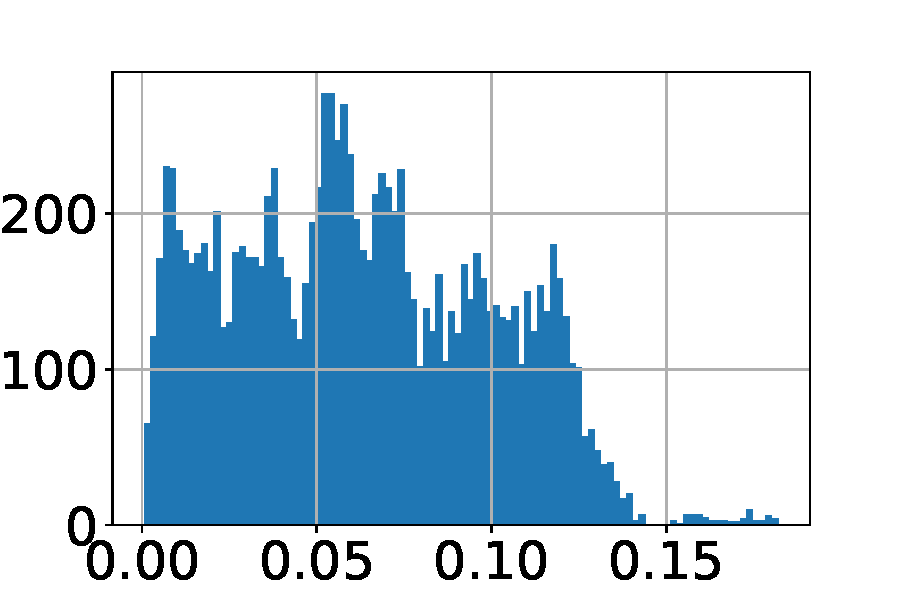
\includegraphics[width=0.22\paperwidth]{Hist_example_Beach.pdf}}
  %
  \subfloat[\label{fig:Hist_example_logBeach}logBeach]
  {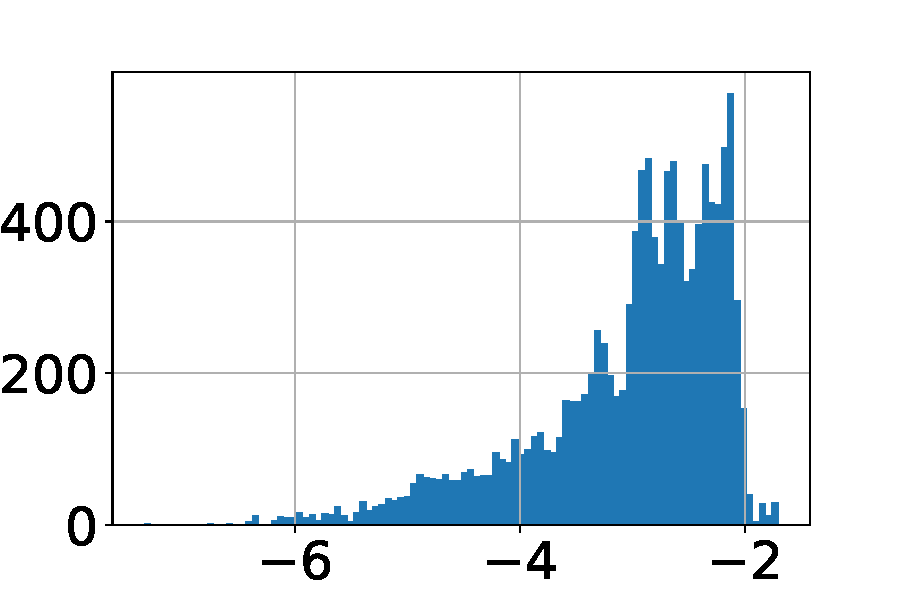
\includegraphics[width=0.22\paperwidth]{Hist_example_logBeach.pdf}}
  %
  \subfloat[\label{fig:Hist_example_logBeach1000}log(Beach$-$1000)]
  {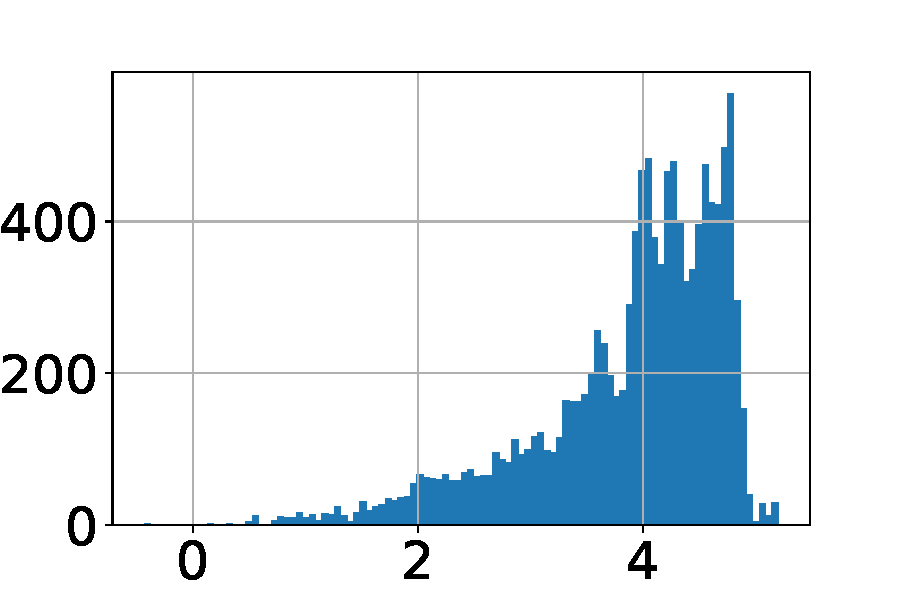
\includegraphics[width=0.22\paperwidth]{Hist_example_logBeach1000.pdf}}

  \subfloat[\label{fig:Hist_example_Gaol}Gaol]
  {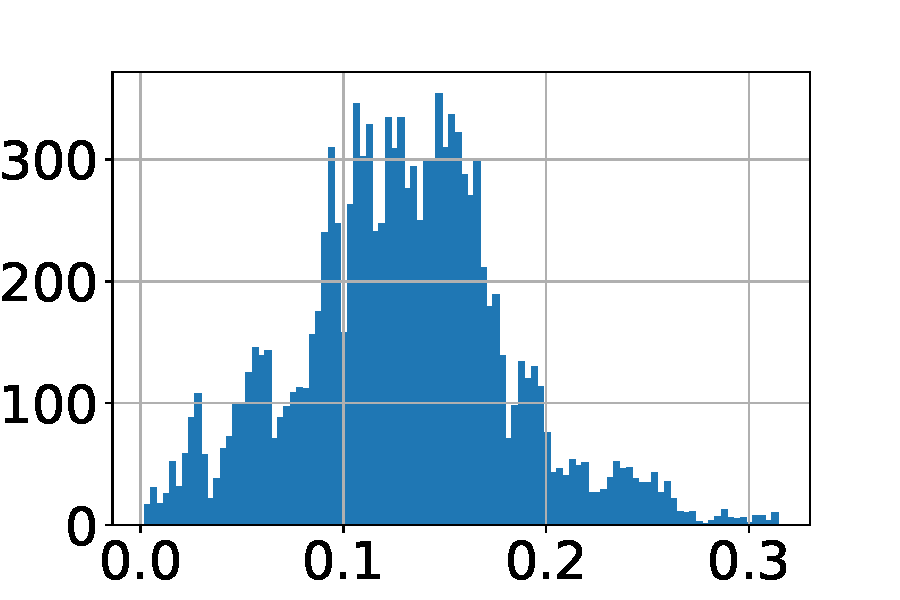
\includegraphics[width=0.22\paperwidth]{Hist_example_Gaol.pdf}}
  %
  \subfloat[\label{fig:Hist_example_logGaol}logGoal]
  {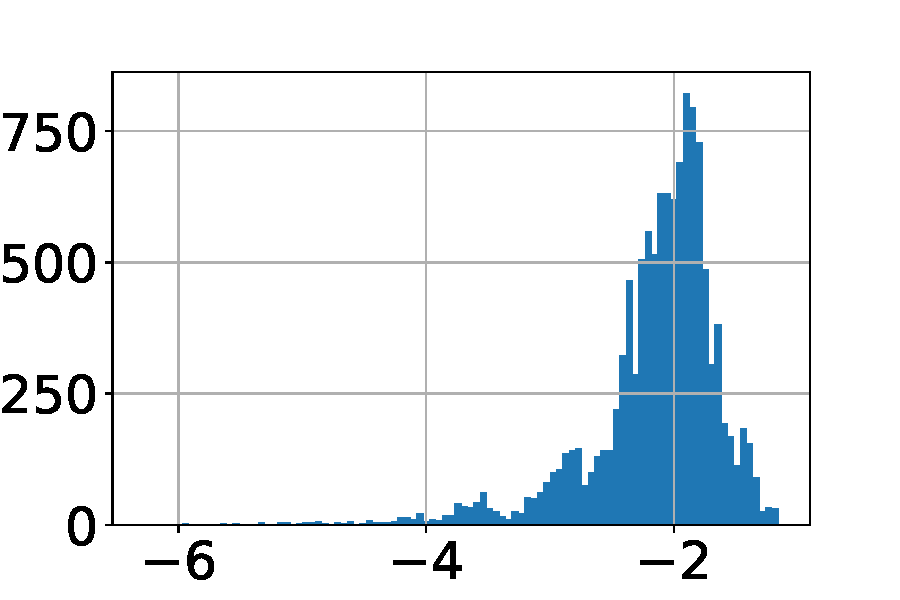
\includegraphics[width=0.22\paperwidth]{Hist_example_logGaol.pdf}}
  %
  \subfloat[\label{fig:Hist_example_logGaol1000}log(Gaol$-$1000)]
  {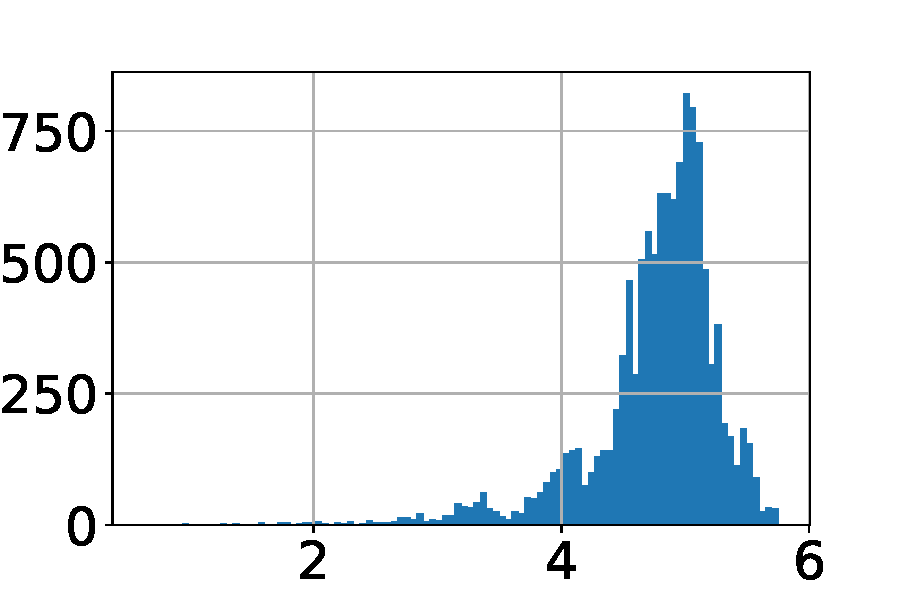
\includegraphics[width=0.22\paperwidth]{Hist_example_logGaol1000.pdf}}
  %
  \caption{Illustration of left-skewness and long tails induced by log transform.}
  \label{fig:Hist_example}
  %
\end{figure}

In the log regression, lasso selects 35 variables and CV-en selects 54. Some of the lasso and CV-en selections seem odd. For example, lasso drops all Year 5 test scores, Year 3 Spelling, and Yearv3 Grammar, but selects all the other Year 3 scores while CV-en selects all the scores except Year 5 Reading. The selections seem to suggest that only some primary school examination scores matter in house pricing. By contrast, solar returns a very sparse regression model, with only 11 variables selected in the log regression, 9 of which are also selected in the linear regression. Since causal relations should not be affected by functional form, we focus on variables selected by solar under linear and log forms in Table~\ref{table:house_variable}: \{bedrooms, baths, Parking, Beach, ChildCare, Gaol, ICSEA, logMortgage, logRent, logFamInc\}.

\begin{table}[h]
  \renewcommand*{\arraystretch}{0.8}
  \centering
  \caption{OLS coefficients: post-selection log model}
  \label{table:coefficients_log}
  %
\resizebox*{!}{1.0\textwidth}{%
  \begin{tabular}{@{}l....@{}}
  %
  \toprule
  Variable & \multicolumn{1}{c}{elas net}
           & \multicolumn{1}{c}{lasso}
           & \multicolumn{1}{c}{rec solar}
           & \multicolumn{1}{c}{solar}      \\
  %
  \midrule
  constant     & 8.81\ts   & 8.76\ts   & 7.99\ts   & 7.21\ts  \\
               &  (0.17)   &  (0.15)   &  (0.11)   &  (0.11)  \\
  Bedrooms     & 0.21\ts   & 0.21\ts   & 0.23\ts   & 0.23\ts  \\
               &  (0.00)   &  (0.00)   &  (0.00)   &  (0.00)  \\
  Baths        & 0.09\ts   & 0.10\ts   & 0.09\ts   & 0.09\ts  \\
               &  (0.00)   &  (0.00)   &  (0.00)   &  (0.00)  \\
  Parking      & 0.08\ts   & 0.08\ts   & 0.08\ts   & 0.08\ts  \\
               &  (0.00)   &  (0.00)   &  (0.00)   &  (0.00)  \\
  Airport      & 3.67\ts   & 2.53\ts   & 2.88\ts   &          \\
               &  (0.39)   &  (0.20)   &  (0.25)   &          \\
  Beach        & -1.78\ts  & -2.21\ts  & -1.34\ts  & -2.45\ts \\
               &  (0.31)   &  (0.11)   &  (0.14)   &  (0.14)  \\
  Child care   & -4.39\ts  & -4.49\ts  & -3.63\ts  & -2.45\ts \\
               &  (0.20)   &  (0.16)   &  (0.12)   &  (0.11)  \\
  Gaol         & -0.80\ds  &           & -1.01\ts  & 0.36\ts  \\
               &  (0.32)   &           &  (0.15)   &  (0.14)  \\
  Rubbish      & -0.4      &           & 0.54\ts   &          \\
               &  (0.35)   &           &  (0.21)   &          \\
  log(Mortgage)& 0.16\ts   & 0.16\ts   & 0.24\ts   & 0.26\ts  \\
               &  (0.01)   &  (0.01)   &  (0.01)   &  (0.01)  \\
  log(Rent)    & 0.03\ts   & 0.04\ts   & 0.07\ts   & 0.07\ts  \\
               &  (0.01)   &  (0.01)   &  (0.01)   &  (0.01)  \\
  log(Income)  & 0.19\ts   & 0.19\ts   & 0.17\ts   & 0.24\ts  \\
               &  (0.02)   &  (0.01)   &  (0.01)   &  (0.01)  \\
  Age          & 0.01\ts   & 0.01\ts   & 0.01\ts   & 0.01\ts  \\
               &  (0.00)   &  (0.00)   &  (0.00)   &  (0.00)  \\
  ICSEA        & 0.00\ts   & 0.00\ts   & 0.00\ts   & 0.00\ts  \\
               &  (0.00)   &  (0.00)   &  (0.00)   &  (0.00)  \\
  $+$          &           &           &           &          \\
  %
  \midrule
  $p$          &     54    &     36    &     13    &     11    \\
  $R^2$        &      0.77 &      0.76 &      0.74 &      0.73 \\
  $\bar{R}^2$  &      0.77 &      0.76 &      0.74 &      0.73 \\
  $n$          & 11,796    & 11,796    & 11,796    & 11,796    \\
  \bottomrule
  \end{tabular}}
  %
\end{table}

\begin{table}[h]
  \renewcommand*{\arraystretch}{0.8}
  \centering
  \caption{OLS coefficients: post-selection linear model}
  \label{table:coefficients_linear}
  %
\resizebox*{!}{1.0\textwidth}{%
  \begin{tabular}{@{}l....@{}}
  %
  \toprule
  Variable & \multicolumn{1}{c}{elas net}
           & \multicolumn{1}{c}{lasso}
           & \multicolumn{1}{c}{rec solar}
           & \multicolumn{1}{c}{solar} \\
  %
  \midrule
  constant   &  -886234.40\ts &  -827387.49\ts & -1445430.40\ts & -2486422.15\ts \\
             &  (186680.91)   &  (174136.59)   &  (112390.24)   &   (98422.98)   \\
  Bedrooms   &   165639.00\ts &   166225.82\ts &   183893.59\ts &   169510.52\ts \\
             &    (6433.57)   &    (6404.82)   &    (6015.93)   &    (6015.37)   \\
  Baths      &   210101.84\ts &   210600.58\ts &   203674.28\ts &   209626.52\ts \\
             &    (8115.07)   &    (8048.92)   &    (8147.93)   &    (8297.24)   \\
  Parking    &    97790.57\ts &    96883.13\ts &   104050.40\ts &    97623.23\ts \\
             &    (6689.35)   &    (6688.13)   &    (6861.16)   &    (6985.67)   \\
  Airport    &  2865246.35\ts &  3122719.74\ts &  1849108.51\ts &                \\
             &  (735335.86)   &  (625604.38)   &  (454344.97)   &                \\
  Beach      & -5029681.74\ts & -4051671.57\ts & -1509612.24\ts &  -796281.77\ts \\
             &  (600061.28)   &  (262369.00)   &  (260370.04)   &  (153431.50)   \\
  Child care & -4802095.18\ts & -4163486.91\ts & -3961629.37\ts &                \\
             &  (393577.54)   &  (316107.89)   &  (220752.57)   &                \\
  Gaol       &  1614215.27\ds &                & -1137143.99\ts & -1909369.80\ts \\
             &  (646392.84)   &                &  (267597.21)   &  (107204.64)   \\
  Rubbish    &   -45084.93    &   780180.22    &  3136997.85\ts &                \\
             &  (672532.42)   &   594084.58)   &  (372355.34)   &                \\
  Mortgage   &      133.67\ts &      134.18\ts &      174.55\ts &      185.99\ts \\
             &       (7.98)   &       (7.95)   &       (7.82)   &       (7.96)   \\
  Rent       &      264.35\ts &      265.80\ts &      312.85\ts &      370.76\ts \\
             &      (36.80)   &      (35.27)   &      (34.78)   &      (35.42)   \\
  Income     &       59.04\ts &       69.22\ts &       -8.39    &       66.57\ts \\
             &      (19.23)   &      (14.97)   &      (12.18)   &      (11.48)   \\
  Age        &     3673.46\ts &     4106.29\ts &                &                \\
             &    (1031.69)   &      (958.98)  &                &                \\
  ICSEA      &      838.54\ts &      862.92\ts &      960.68\ts &     1756.92\ts \\
             &     (172.42)   &     (163.42)   &     (104.07)   &      (95.67)   \\
  $+$        &                &                &                &                \\
  %
  \midrule
  $p$         &       57      &        44      &       12       &        9       \\
  $R^2$       &        0.548  &         0.548  &        0.514   &        0.494   \\
  $\bar{R}^2$ &        0.546  &         0.546  &        0.514   &        0.493   \\
  $n$         &   11,974      &     11,974     &   11,974       &   11,974       \\
  \bottomrule
  \end{tabular}}
  %
\end{table}

Lastly, solar outperforms the lasso-type estimators in terms of the balance between sparsity and prediction accuracy. Table~\ref{table:coefficients_linear} shows the post-selection OLS results based on CV-en, lasso, and solar selection from the log models; solar selects only 9 variables compared with lasso (44) and CV-en (57). Surprisingly, pruning 35 to 48 variables from the \ref{table:house_variable} list reduces the $R^2$ by only 5\%. This confirms that, solar successfully identifies the most important predictive variables in the database. A similar result occurs in Table~\ref{table:coefficients_log}, where solar only selects 11  variables that explain 73\% of the variation in log(price). Comparing solar to lasso, the 25 extra variables increase $R^2$ by only 3\%. This suggests either that the 3\% gain is due to overfitting; or that the extra variables are only weakly conditionally correlated to $\log \left( \mathrm{Price} \right)$. The Markov Blanket variables of $\log \left( \mathrm{Price} \right)$, which have direct causal relations to and from $\log \left( \mathrm{Price} \right)$, are always strongly correlated to $\log \left( \mathrm{Price} \right)$, holding all other variables constant. Variables with a weak conditional correlation, therefore, may be only remote ancestors or descendants of $\log \left( \mathrm{Price} \right)$. This is not to say they have no causal relation to $\log \left( \mathrm{Price} \right)$; it just implies that they are not in the MB of $\log \left( \mathrm{Price} \right)$ and have no direct causal effect.

While the linear and log models should represent the same causal structure, the linear model performs relatively poorly. Since the dollar measured variables are less skewed and possibly with a lighter tail under logs, we focus on the log regression. As explained previously, the MB includes all the variables that are conditionally correlated to price in the population, implying that the MB variables should be able to explain all non-noise variation in price. Since we do not know the population variance of noise, we cannot know with absolute certainty the magnitude of noise variation. However, with $R^2=73$\%, we are confident that the majority of price variation is linear and explained by the MB. The remaining 27\% may be due to noise, functional form error, or spatial clustering in the geographical data.\footnote{For example, to capture nonlinear patterns, we could use a polynomial equation, a trigonometric equation, or a neural network instead of a first-order linear equation.} While we cannot rule out nonlinearity, the severity of these problems appears to be under control. The high explanatory power of the variables selected by solar under the log transform is reassuring when it comes to the reliability of MB selection. In Appendix~3, we try using other machine learning methods to capture nonlinearity between $\log \left( \mathrm{price} \right)$ and the selected $11$ variables. \textcolor[rgb]{0.00,0.00,1.00}{It turns out that, with cross-validation controlling for overfitting, the selected variables can easily explain about 90\% of the variation in $\log \left( \mathrm{price} \right)$, confirming that there is a nonlinear relation between the selected variables and $\log \left( \mathrm{price} \right)$, which accounts for another 17\% of $R^2$ and is not the major pattern in our dataset.}

\subsection{Grouping effects in variable selection}

Before moving to graph learning, it is important to check whether grouping effects cause solar to mistakenly exclude variables from the price MB. As noted above, variable selection accuracy and robustness may be reduced when grouping effects are present in the data, and especially when the dependence and causation structures are complicated. As shown in the supplementary correlation table, the distances of houses to different locations are highly spatially correlated with one another. To investigate whether solar variable selection is affected by this multicollinearity, Table~\ref{table:corr_gaol} focuses on the group of variables that are highly correlated with gaol, including airport, rubbish, and childcare, all of which have pairwise unconditional correlations above 0.5.

\begin{table}[H]
 %
 \small
 \centering
 \caption{Unconditional correlations with Gaol (absolute value $> 0.5$) \label{table:corr_gaol}}
 %
 \begin{tabular}{lcccc.}
  %
  \toprule
  %
    & ChildCare & Airport & Rubbish & Beach \\
  %
  \midrule
  %
  $\mathrm{corr}\left(\;\cdot\;,\mathrm{Gaol}\right)$ & 0.756 & 0.715 & 0.671 & 0.528 \\
  %
  \bottomrule
  %
 \end{tabular}
 %
\end{table}

Based on the Table~\ref{table:corr_gaol} results, we standardize all variables and estimate the regression
%
\begin{equation}
 %
 \mathrm{Gaol} = \gamma_0 + \gamma_1 \cdot \mathrm{Airport} + \gamma_2 \cdot \mathrm{ChildCare} + \gamma_3 \cdot \mathrm{Rubbish} + \gamma_4 \cdot \mathrm{Beach} + e.
 %
 \label{OLS:Gaol_others}
 %
\end{equation}
%
The estimation results from (\ref{OLS:Gaol_others}) are in Table~\ref{table:OLS_gaol}.

\begin{table}[H]
 %
 \renewcommand*{\arraystretch}{0.8}
 \small
 \centering
 \caption{OLS results from (\ref{OLS:Gaol_others}) \label{table:OLS_gaol}}
 %
\begin{tabular}{r....}
  %
  \toprule
            & \multicolumn{1}{c}{coefficient}
            & \multicolumn{1}{c}{$SE$}
            & \multicolumn{1}{c}{$t $}
            & \multicolumn{1}{c}{$P>|t|$} \\
  %
  \midrule
  constant  & 0      & 0.003   & 0       & 1.000 \\
  Airport   & 0.4488 & 0.011   & 41.063  & 0.000 \\
  ChildCare & 0.3276 & 0.006   & 56.908  & 0.000 \\
  Rubbish   & 0.0373 & 0.010   & 3.849   & 0.000 \\
  Beach     & 0.5522 & 0.003   & 174.257 & 0.000 \\
  \bottomrule
  %
 \end{tabular}
 %
 \begin{tabular}{r.r.}
  %
  $n$          & 11,974 & $F$                & 23,110 \\
  $R^2$        & 0.885  & $P(F)$             & 0      \\
  $\bar{R}^2$  & 0.885  & degrees of freedom & 4      \\
  \bottomrule
  %
\end{tabular}
%
\end{table}

Table~\ref{table:OLS_gaol} shows that almost 90\% of the variation in Gaol is explained by \{ChildCare, Airport, Rubbish, Beach\} with $\sum_{\forall i \neq 0} \left\vert \hat{\gamma}_i \right\vert = 1.35$, indicating severe multicollinearity between Gaol and the other 4 variables. The empirical reason \{Gaol, ChildCare, Airport, Rubbish, Beach\} are highly correlated is easy to see. The house data cover a roughly 10km square area in eastern Sydney. The gaol (Long Bay correctional complex), several childcare centers (e.g., Blue Gum Cottage Child Care, Alouette Child Care, etc.), the airport (Kingsford-Smith Airport), and waste treatment facilities (e.g., Banksmeadow Transfer Terminal, Malabar Wastewater Treatment Plant, Cronulla Wastewater Treatment Plant) are all located in the southeast corner of the 10km square, explaining the collinearity among the variables.

The multicollinearity very likely breaches the IRC and indicates the presence of grouping effects, casting doubt on the variable selection process. The implication is that, even though we know that at least one of \{ChildCare, Airport, Rubbish, Beach, Gaol\} is in the MB of price, it may be difficult statistically to pinpoint which one. To avoid being misled by a grouping effect, we expand the subset \{Gaol, ChildCare, Beach\} to \{Gaol, ChildCare, Beach, Airport, Rubbish\} and refer to the latter as the `rectified' solar selection. For completeness, we compare the OLS results in linear and log forms with the selection results from lasso, CV-en, solar ((\ref{OLS:solar}) and (\ref{OLS:solar_log})), and rectified solar ((\ref{OLS:postsolar}) and (\ref{OLS:postsolar_log})).
%
\begin{align}
  %
  \mathrm{Price} = \beta_0 & + \beta_1 \cdot \mathrm{Mortgage} + \beta_2 \cdot \mathrm{Rent} +
  \beta_3 \cdot \mathrm{FamInc} + \beta_4 \cdot \mathrm{Bedrooms} \label{OLS:solar} \\
  & + \beta_5 \cdot \mathrm{Baths} + \beta_6 \cdot \mathrm{Parking} + \beta_7 \cdot \mathrm{Beach} + \beta_8 \cdot \mathrm{Gaol} + \beta_9 \cdot \mathrm{ICSEA} + u; \notag \\
  %
  \mathrm{Price} = \beta_0 & + \beta_1 \cdot \mathrm{Mortgage} + \beta_2 \cdot \mathrm{Rent}
  + \beta_3 \cdot \mathrm{FamInc} + \beta_4 \cdot \mathrm{Bedrooms}  \label{OLS:postsolar} \\
  & + \beta_5 \cdot \mathrm{Baths} + \beta_6 \cdot \mathrm{Parking}  + \beta_7 \cdot \mathrm{Beach} + \beta_8 \cdot \mathrm{Airport} + \beta_9 \cdot \mathrm{ChildCare} \notag   \\
  & + \beta_{10} \cdot \mathrm{Rubbish} + \beta_{11} \cdot \mathrm{ICSEA} + u; \notag
  %
\end{align}
\begin{align}
  %
  \mathrm{logPrice} = \beta_0 & + \beta_1 \cdot \mathrm{logMortgage} +
  \beta_2 \cdot \mathrm{logRent} + \beta_3 \cdot \mathrm{logFamInc} + \beta_4 \cdot \mathrm{Bedrooms} \label{OLS:solar_log} \\
  & + \beta_5 \cdot \mathrm{Baths} + \beta_6 \cdot \mathrm{Parking} + \beta_7 \cdot \mathrm{Beach} + \beta_8 \cdot \mathrm{Gaol} + \beta_9 \cdot \mathrm{ICSEA} + u; \notag \\
  %
  \mathrm{logPrice} = \beta_0 & + \beta_1 \cdot \mathrm{logMortgage}
  + \beta_2 \cdot \mathrm{logRent}
  + \beta_3 \cdot \mathrm{logFamInc} + \beta_4 \cdot \mathrm{Bedrooms}  \label{OLS:postsolar_log} \\
  & + \beta_5 \cdot \mathrm{Baths} + \beta_6 \cdot \mathrm{Parking}  + \beta_7 \cdot \mathrm{Beach} + \beta_8 \cdot \mathrm{Airport} + \beta_9 \cdot \mathrm{ChildCare} \notag   \\
  & + \beta_{10} \cdot \mathrm{Rubbish} + \beta_{11} \cdot \mathrm{ICSEA} + u. \notag
  %
\end{align}

The comparisons are summarized in Tables~\ref{table:coefficients_log} and \ref{table:coefficients_linear}. The difference between the solar and CV-en $R^2$ values tells us that the 48 variables dropped by solar explain a mere 5\% of price variation while the difference between the solar and rectified solar $R^2$ shows that the gaol group dropped by solar explains 2\% of price variation. A very similar result can be found in the $R^2$ comparison of log models. Thus, among all the 48 dropped variables, \{Airport, Rubbish\} seem to be the most important. This is additional evidence to justify concerns about the grouping effect.

\section{Score-based graph learning based on solar selection}

In last section, we selected the MB of house prices using rectified solar. Ceteris paribus, each variable selected is highly likely to be conditionally correlated to price in the population, implying that they are highly likely to be the MB of price. However, it is possible that these variables have different roles: some may serve as the parents of price while others may serve as children or spouses. In order to accomplish endogeneity detection and instrument variable selection, we need to estimate the role of each MB member along with the complete pattern of causations in the MB. For this step, we implement the score-based graph learning method.

\subsection{Temporal ordering of MB variables and Markov equivalence}

Markov equivalence is a common problem in graph learning and causal inference. In a nutshell, Markov equivalence says that, without an exact time stamp (i.e., when a variable is generated or its value is determined), we cannot learn an exact population graph from data. Instead, we can only learn a skeleton of the population graph (i.e., a graph without arrows or an undirected graph). Figure~\ref{fig:Markov_Equi} illustrates the concept in a simple example.

\begin{figure}[H]
  %
  \centering
  %
  \subfloat[\label{fig:Markov_Equi1}population graph]
  {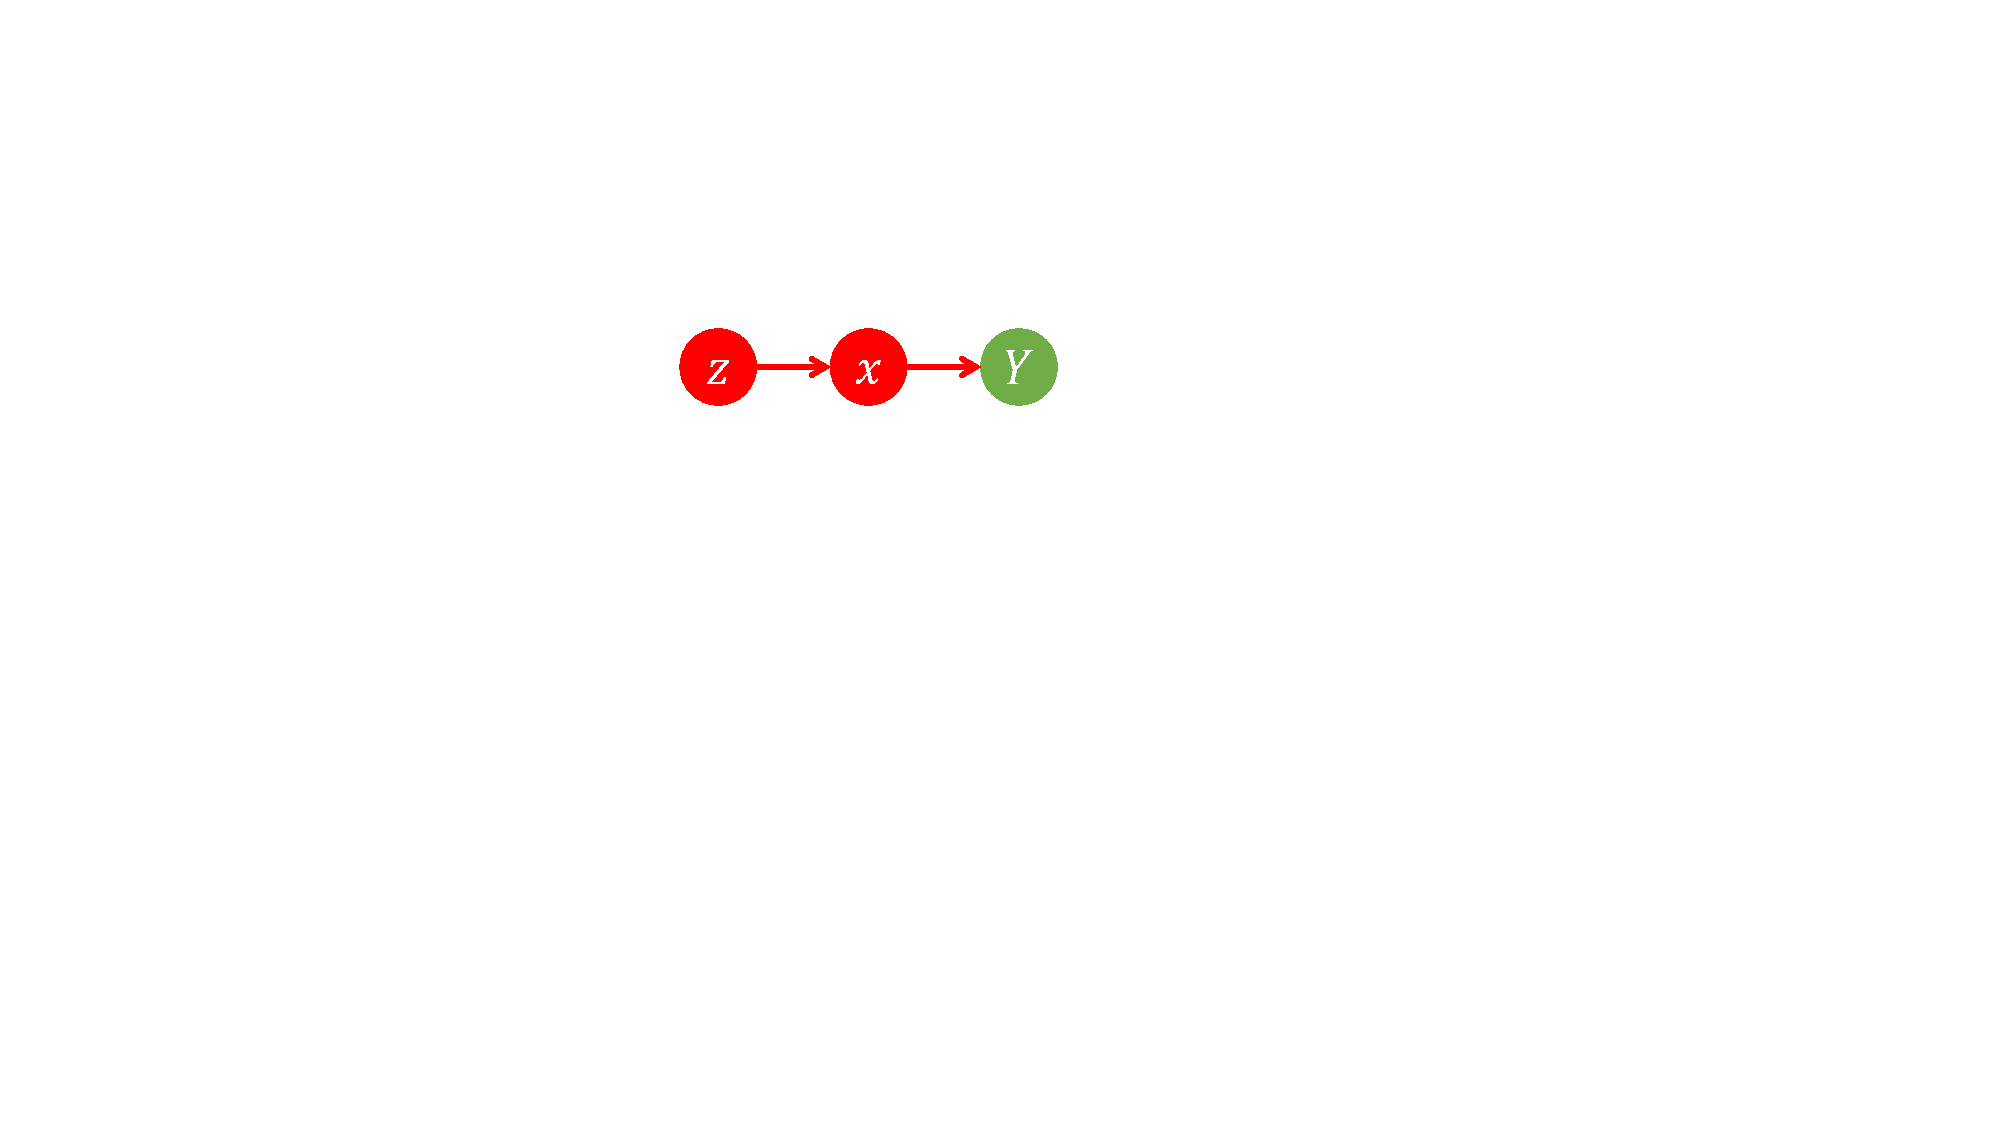
\includegraphics[width=0.2\paperwidth]{ME1.pdf}}
  \hfil
  \subfloat[\label{fig:Markov_Equi2}skeleton of the population graph]
  {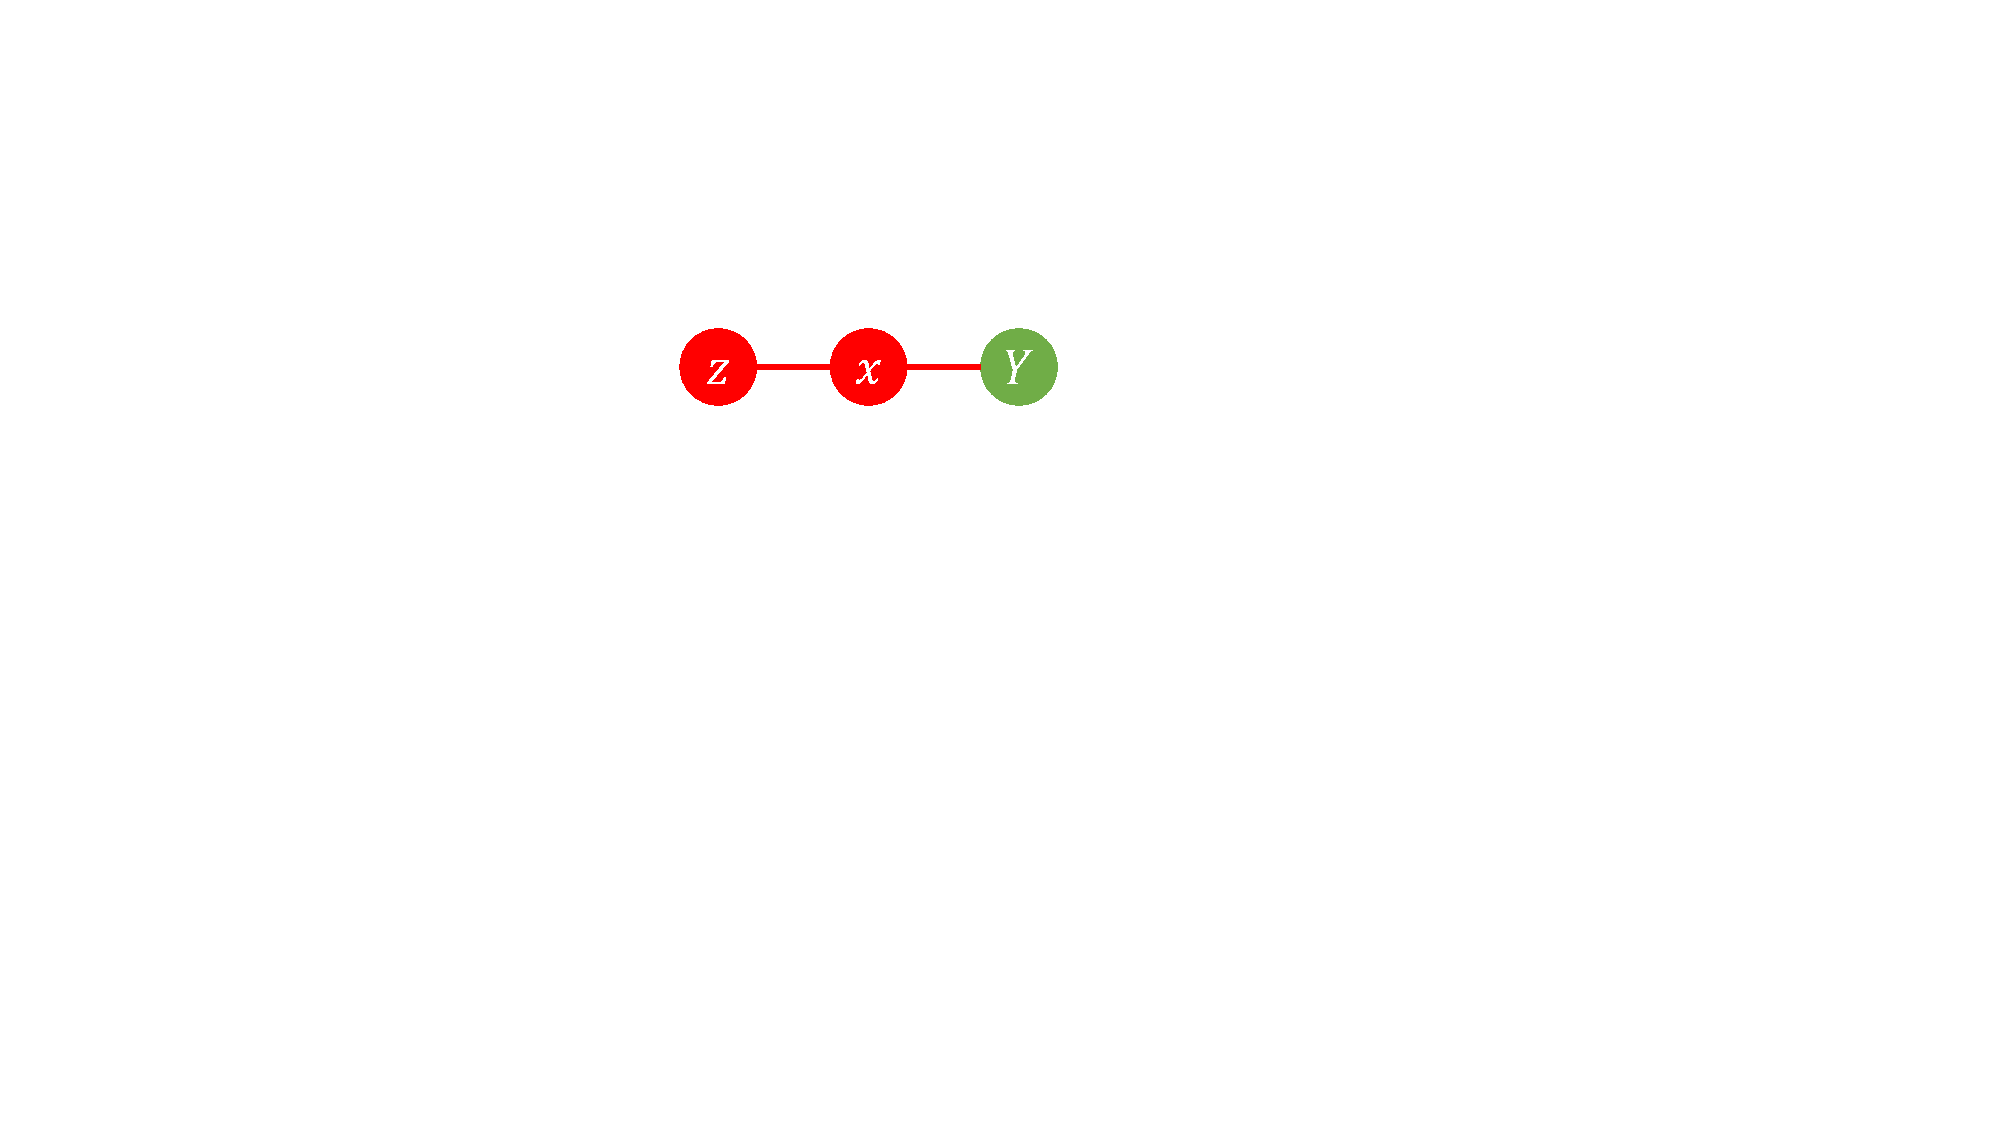
\includegraphics[width=0.2\paperwidth]{ME2.pdf}}
  \hfil
  \subfloat[\label{fig:Markov_Equi3}Markov equivalence 1]
  {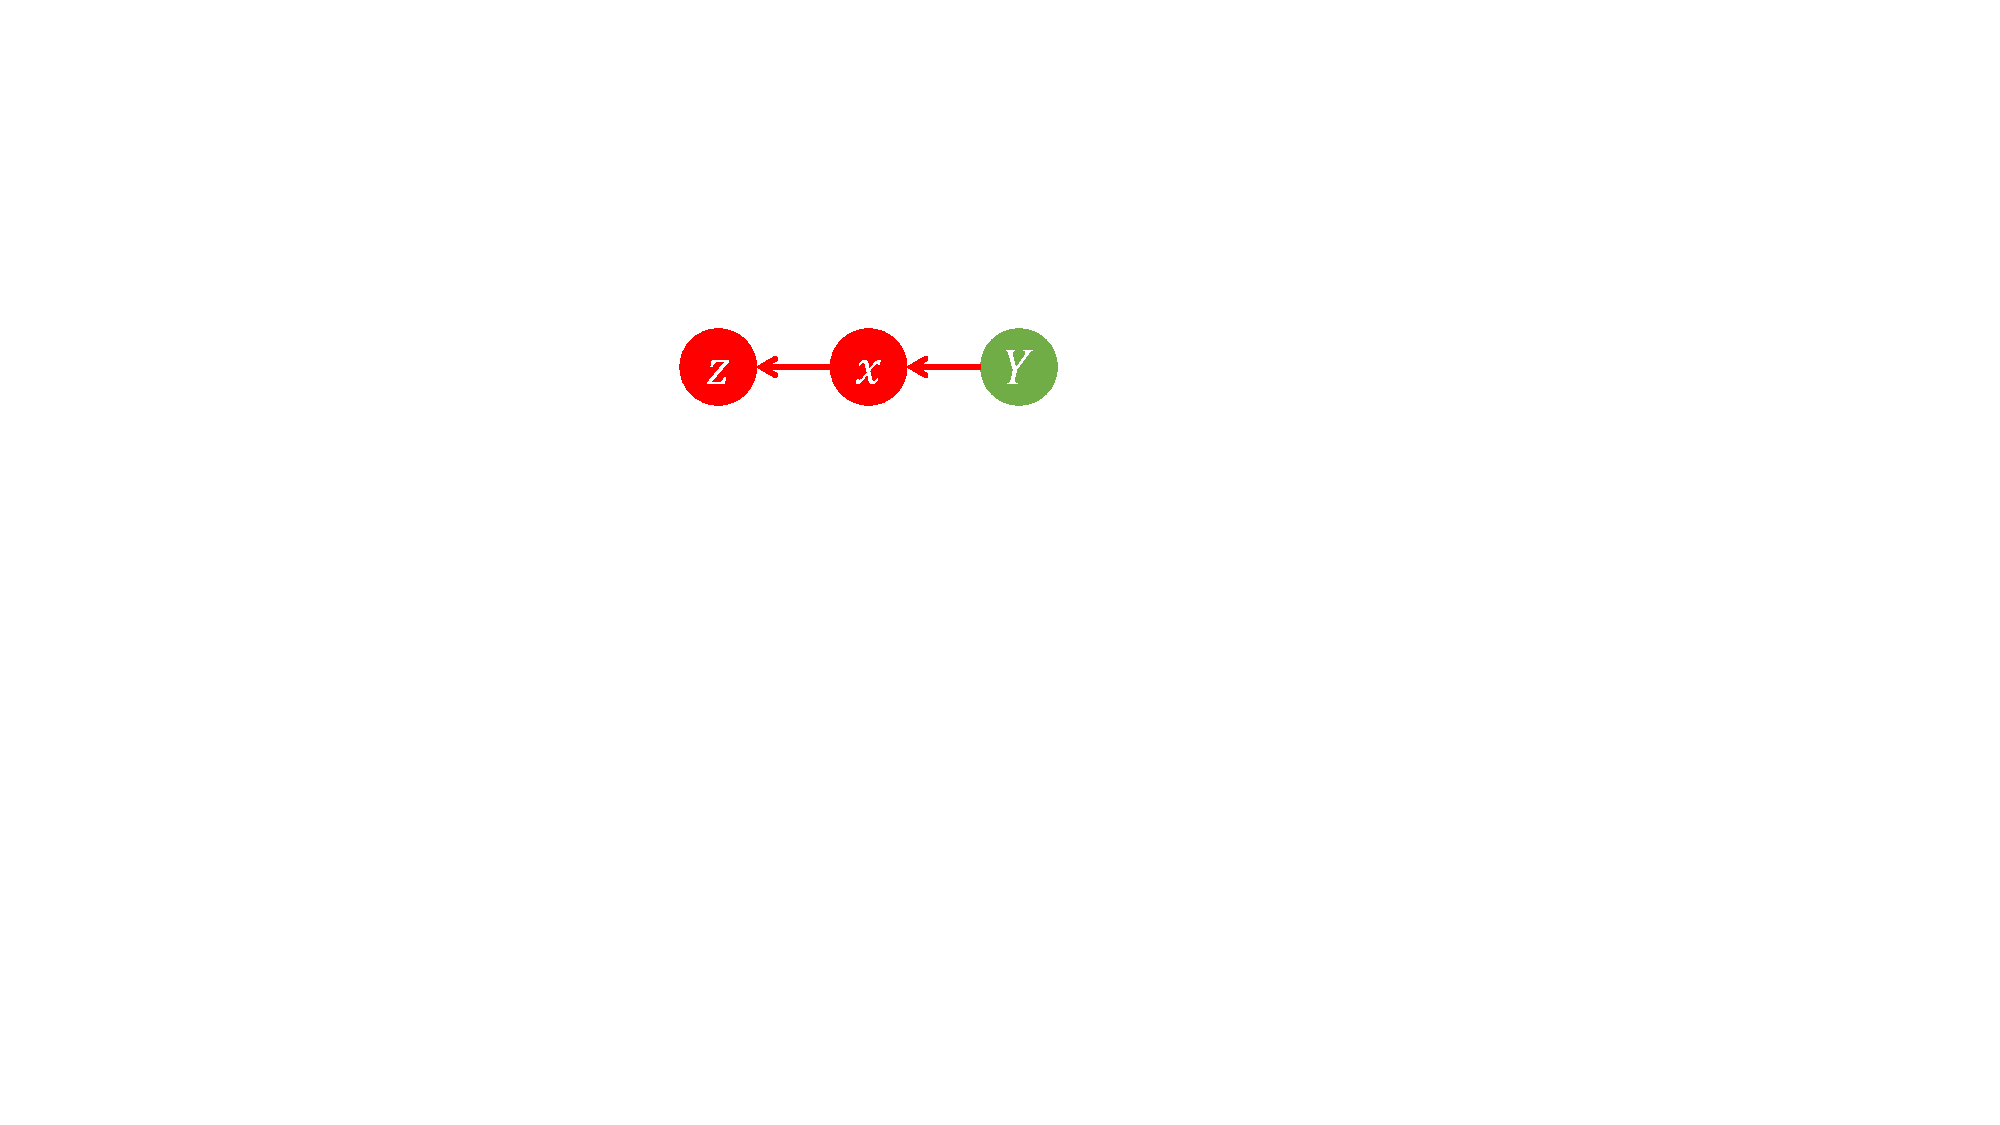
\includegraphics[width=0.2\paperwidth]{ME3.pdf}}

  \subfloat[\label{fig:Markov_Equi4}Markov equivalence 2]
  {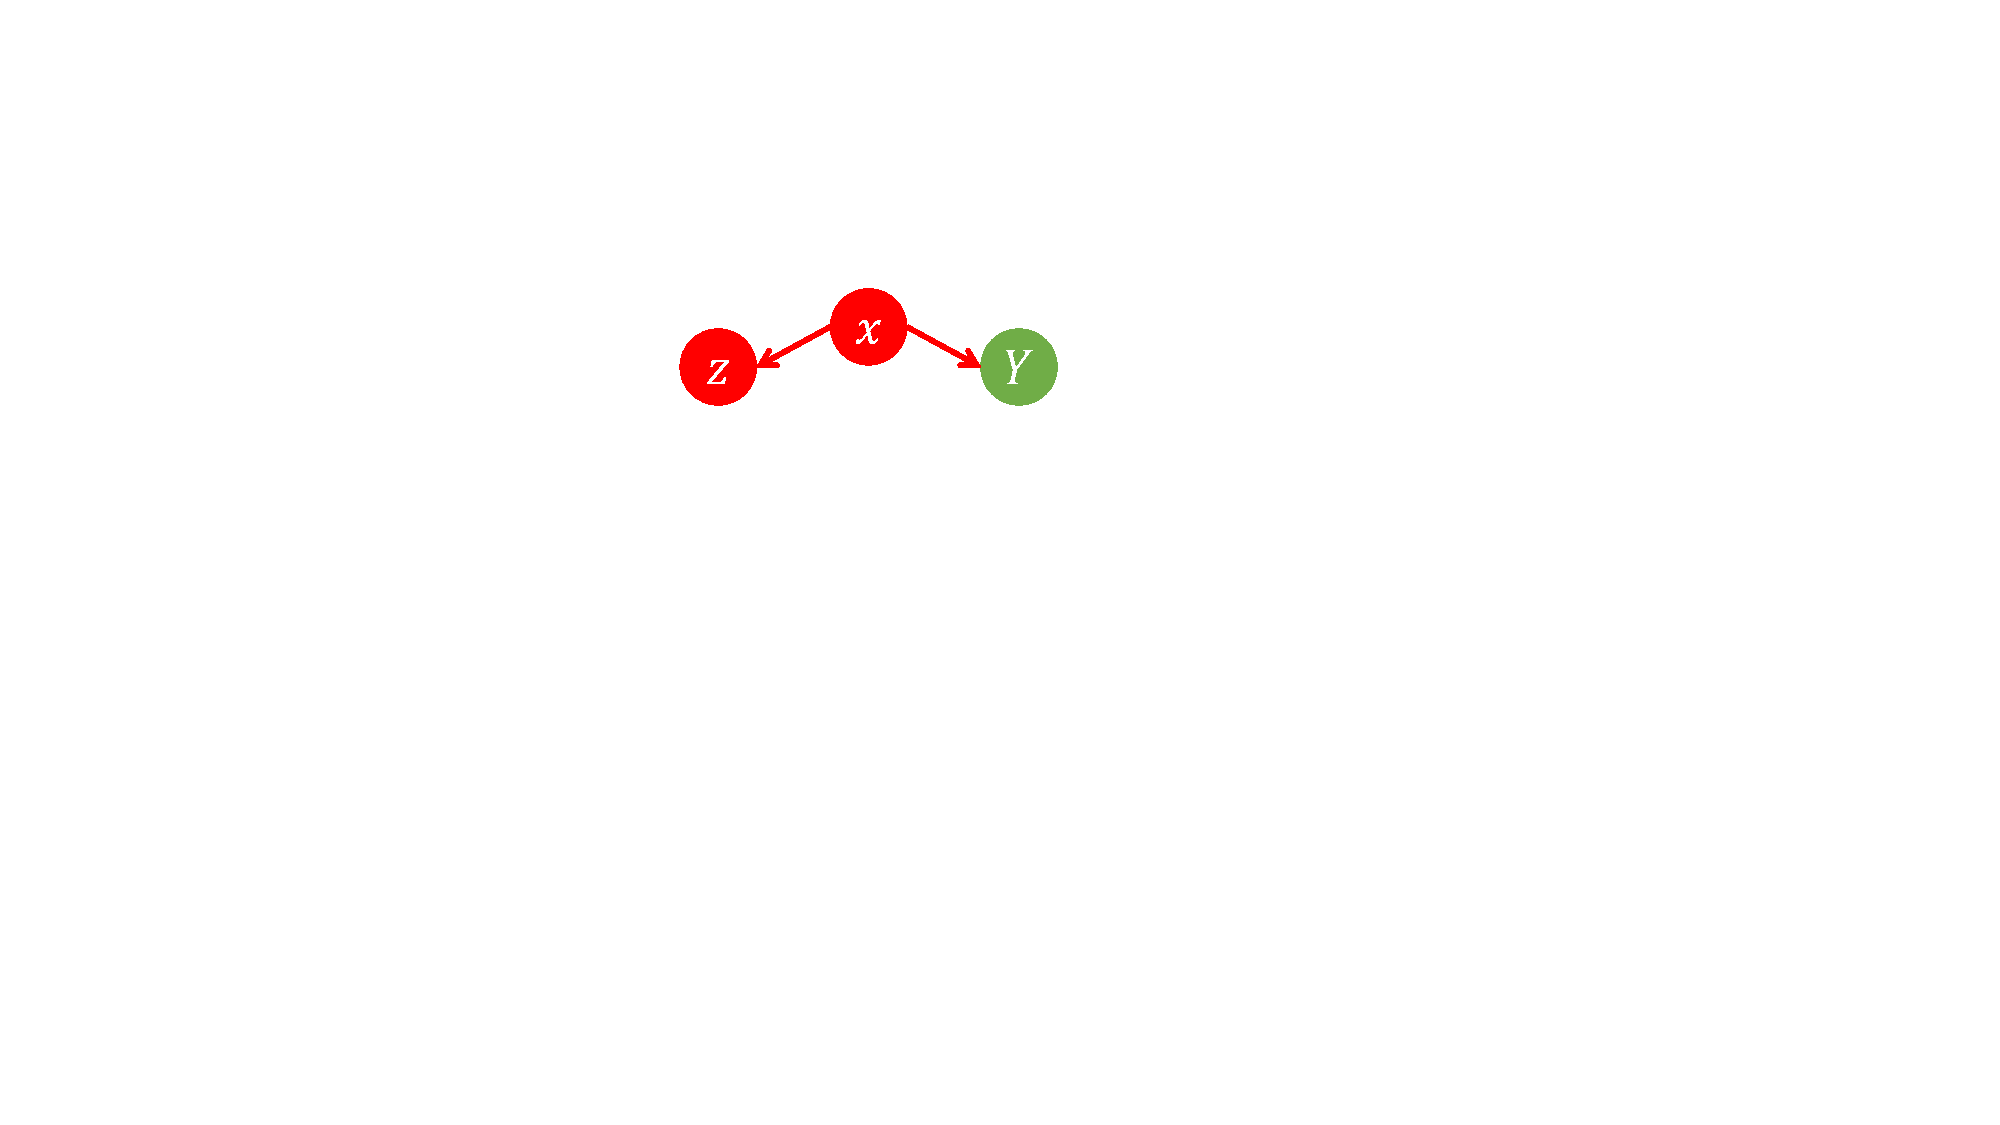
\includegraphics[width=0.25\paperwidth]{ME5.pdf}}
  \hfil
  \subfloat[\label{fig:Markov_Equi5}non-Markov-equivalence]
  {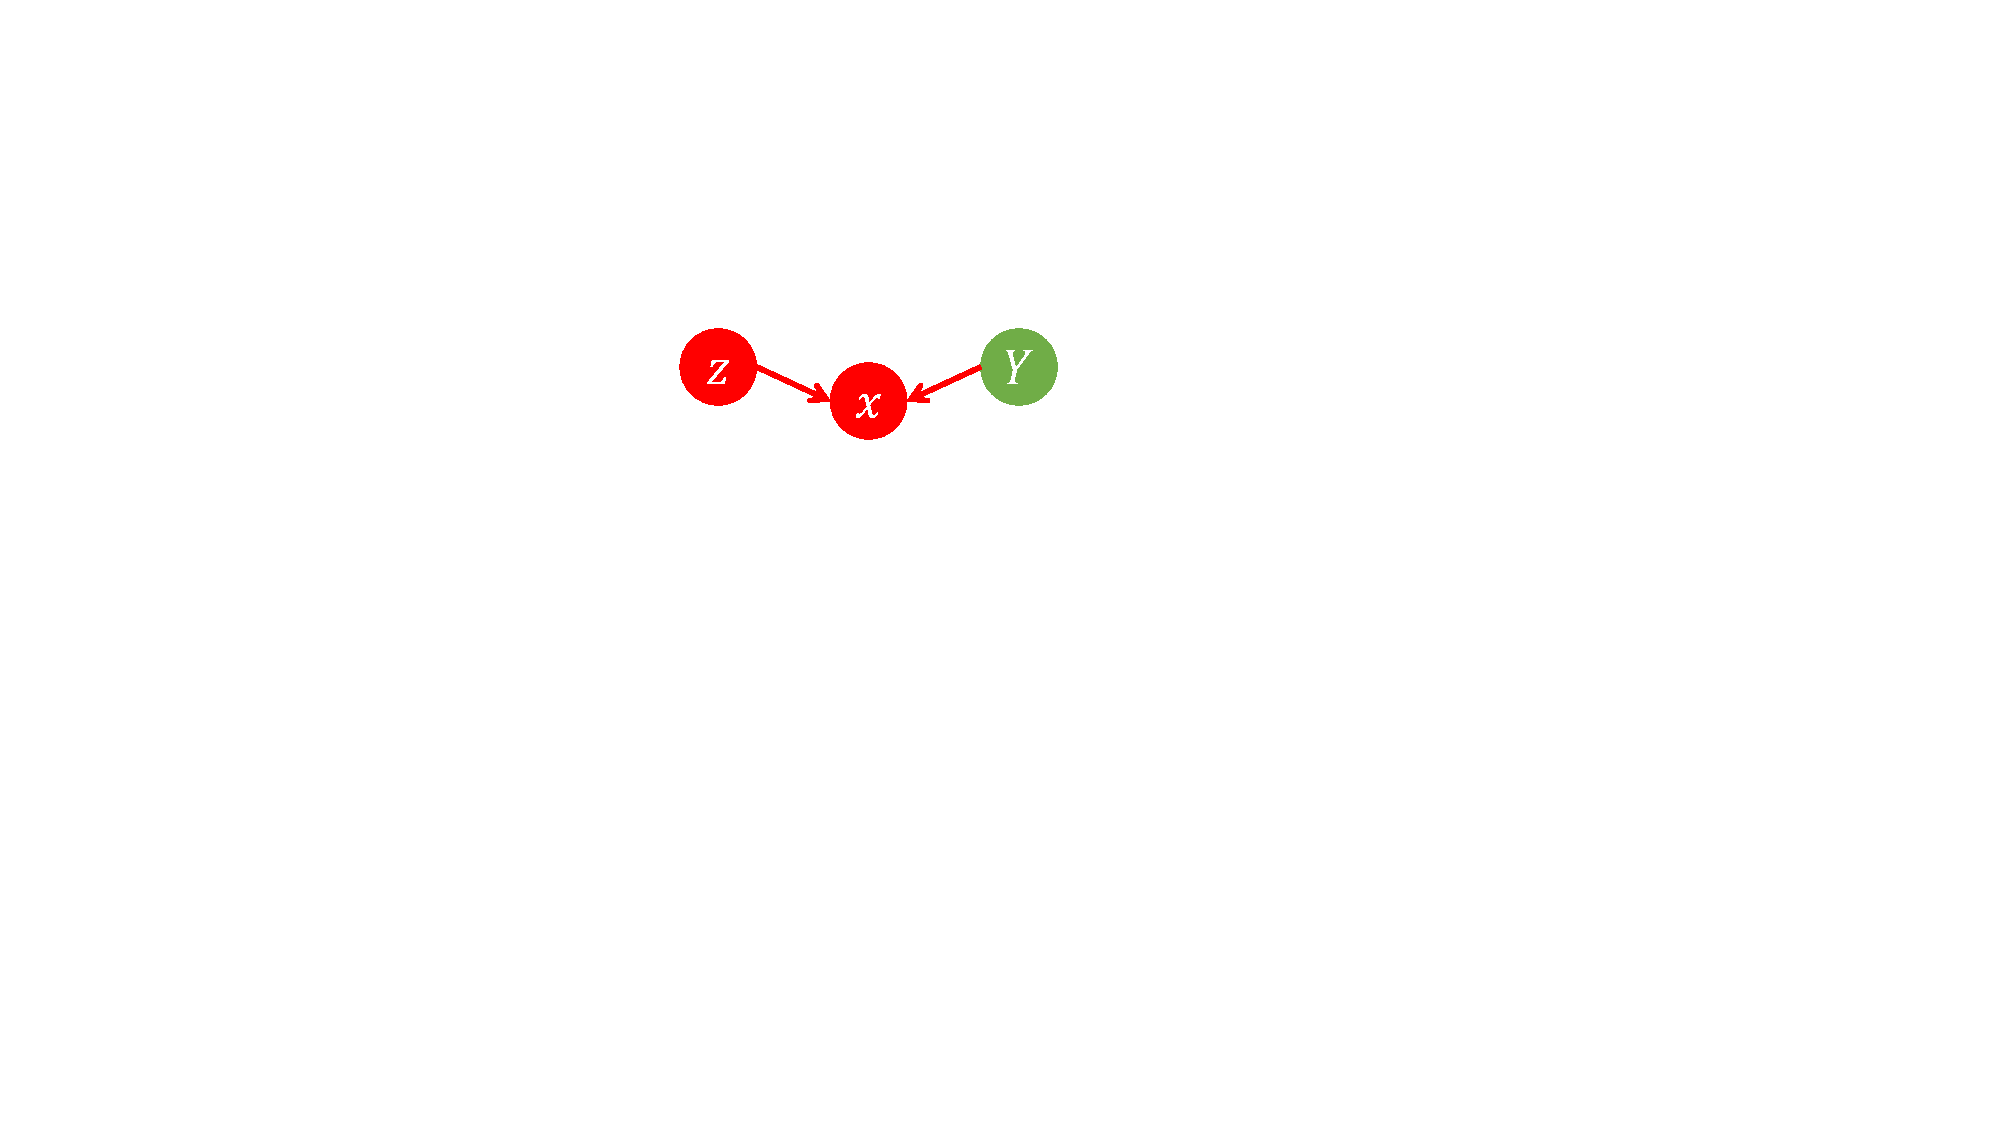
\includegraphics[width=0.25\paperwidth]{ME4.pdf}}
  %
  \caption{Illustration of Markov equivalence.}
  %
  \label{fig:Markov_Equi}
  %
\end{figure}

Figure~\ref{fig:Markov_Equi1} shows the population graph is $\mathbf{z} \rightarrow \mathbf{x} \rightarrow \mathbf{y}$. However, without knowing the time stamp of each variable, it is impossible to find the correct parent-child relations. We can only find a skeleton graph (Figure~\ref{fig:Markov_Equi2}), where we know that $\mathrm{corr} \left( \mathbf{z}, \mathbf{x}\right) \neq 0$, $\mathrm{corr} \left( \mathbf{z}, \mathbf{y} \right) \neq 0$, $\mathrm{corr} \left( \mathbf{y}, \mathbf{x}\right) \neq 0$ and $\mathrm{corr} \left( \mathbf{y} \vert \mathbf{x}, \ \mathbf{z} \vert \mathbf{x} \right) = 0$. Any graphs that fit these conditions are included in the Markov equivalence class. Thus, Figure~\ref{fig:Markov_Equi1} (population graph), Figure~\ref{fig:Markov_Equi3} and Figure~\ref{fig:Markov_Equi4} (the confounding or fork structure) are included in the Markov equivalence class. Figure~\ref{fig:Markov_Equi5} (the collider structure) is not included since the correlation between $\mathbf{z}$ and $\mathbf{y}$ is zero unless $\mathbf{x}$ is conditioned on.

Put another way, without specific time stamps, graph learning can only identify whether or not the population graph follows a collider structure, which is not particularly useful. However, with the corresponding time stamps and a large number of variables, we can eliminate Markov equivalence and narrow the list of candidates in the population graph. For example, if we know that $\mathbf{z}$, $\mathbf{x}$ and $\mathbf{y}$ were generated, respectively, at years 1990, 1991, and 1992, we can rule out Figure~\ref{fig:Markov_Equi3} and \ref{fig:Markov_Equi4} from the Markov Equivalence, implying that Figure~\ref{fig:Markov_Equi1} is the correct graph.

\begin{figure}[H]
  %
  \centering
  %
  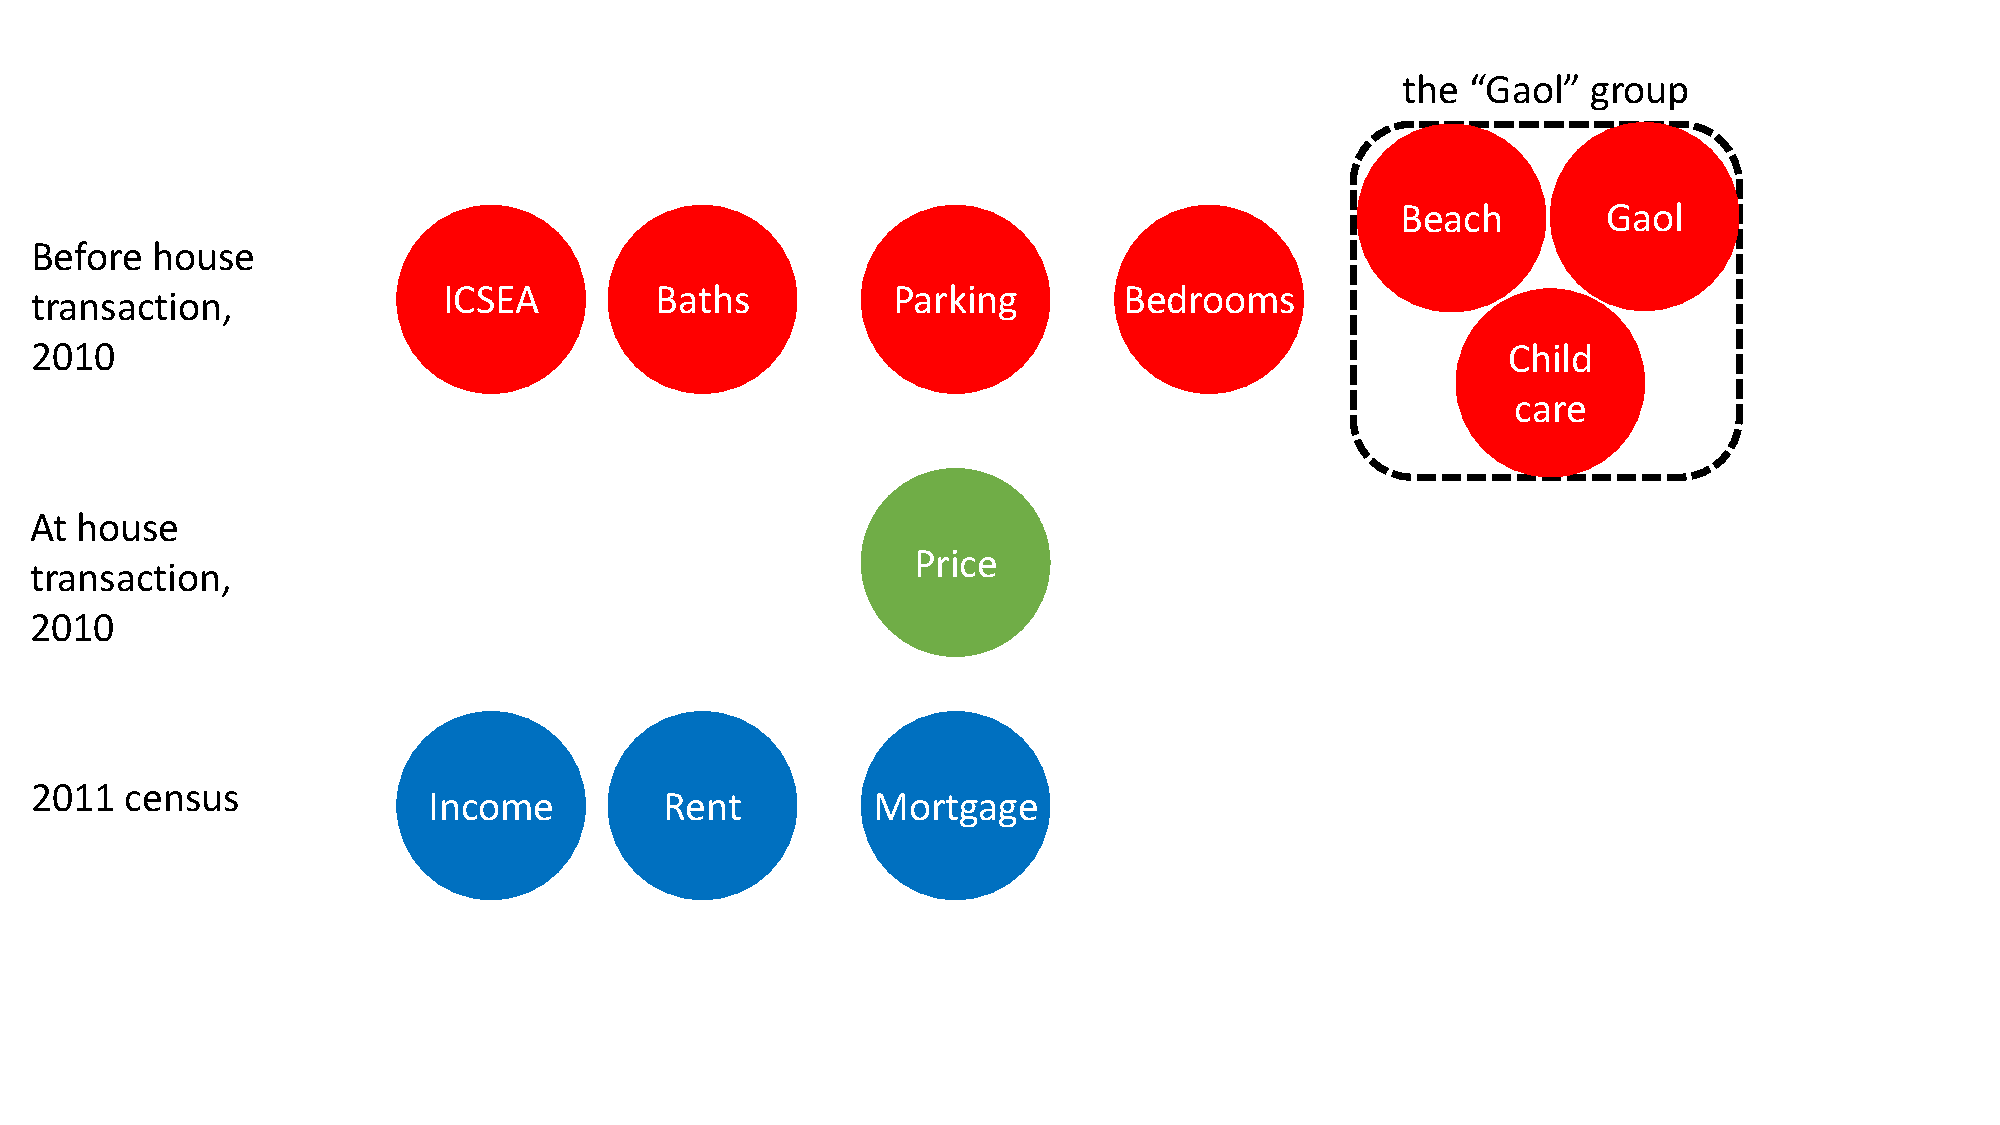
\includegraphics[width=0.6\paperwidth]{BN_pre.pdf}
  %
  \caption{Chronology of variables in the MB of price.}
  %
  \label{fig:BN_pre}
  %
\end{figure}

Based on the time stamps in the house data, the selected variables can be ordered vertically. In Figure~\ref{fig:BN_pre}, the red nodes (house features, distances, and ICSEA) are determined before the house transaction in 2010; the green nodes are generated at the time of the 2010 house transaction; and the blue nodes (demographic variables) are generated at the 2011 census, after the 2010 house transactions.\footnote{Multiple green nodes are included in our database, including the house transaction method (e.g., auction, private sale, and so on), the listing history and 30 or so other variables. We focus on price in this graph estimation.}
Due to the probable IRC violation discussed above, \{Gaol, ChildCare, Beach\} are grouped manually and represent the the `Gaol group' \{Gaol, ChildCare, Beach, Airport, Rubbish\}.

The temporal order helps to identify the role of each variable in the MB: variables generated in 2011 cannot cause any change in those generated in or before 2010, implying that the red nodes cannot be the descendants of green and blue nodes; likewise, the green nodes cannot be the children of blue nodes as well. Since all selected variables are in the MB of price, the red nodes must be the parents of price while rent and mortgage must be the children of price. Since parents cause children, who further cause grandchildren, the time stamps and MB variables yield the estimated graph and the causation relations displayed in Figure~\ref{fig:BN_post}.

The role of income in Figure~\ref{fig:BN_post} is worthy of discussion. The 2009 ICSEA is computed partially based on household income in 2009 while the income variable is observed in 2011. Since there exists a strong intertemporal correlation in household income and since we do not have detailed data on household income, we cannot determine whether the correlation between ICSEA and income is purely autocorrelation or contains some kind of causation. Assuming there is causation, it cannot be identified statistically in the absence of income data linked to house transactions, which are beyond our scope.\footnote{Indeed, it is hard to imagine of a public database that would link house sales to buyer incomes, owing to data privacy protocols.} Hence, we join ICSEA and income with an undirected dash, meaning graphically that there may be a relation that we cannot identify in detail. Since solar variable selection confirms that income and the gaol group belong to both the MB of rent and MB of mortgage (details can be found in the supplementary files), we connect them to rent and mortgage directly, which completes Figure~\ref{fig:BN_post}.

\begin{figure}[h]
  %
  \centering
  %
  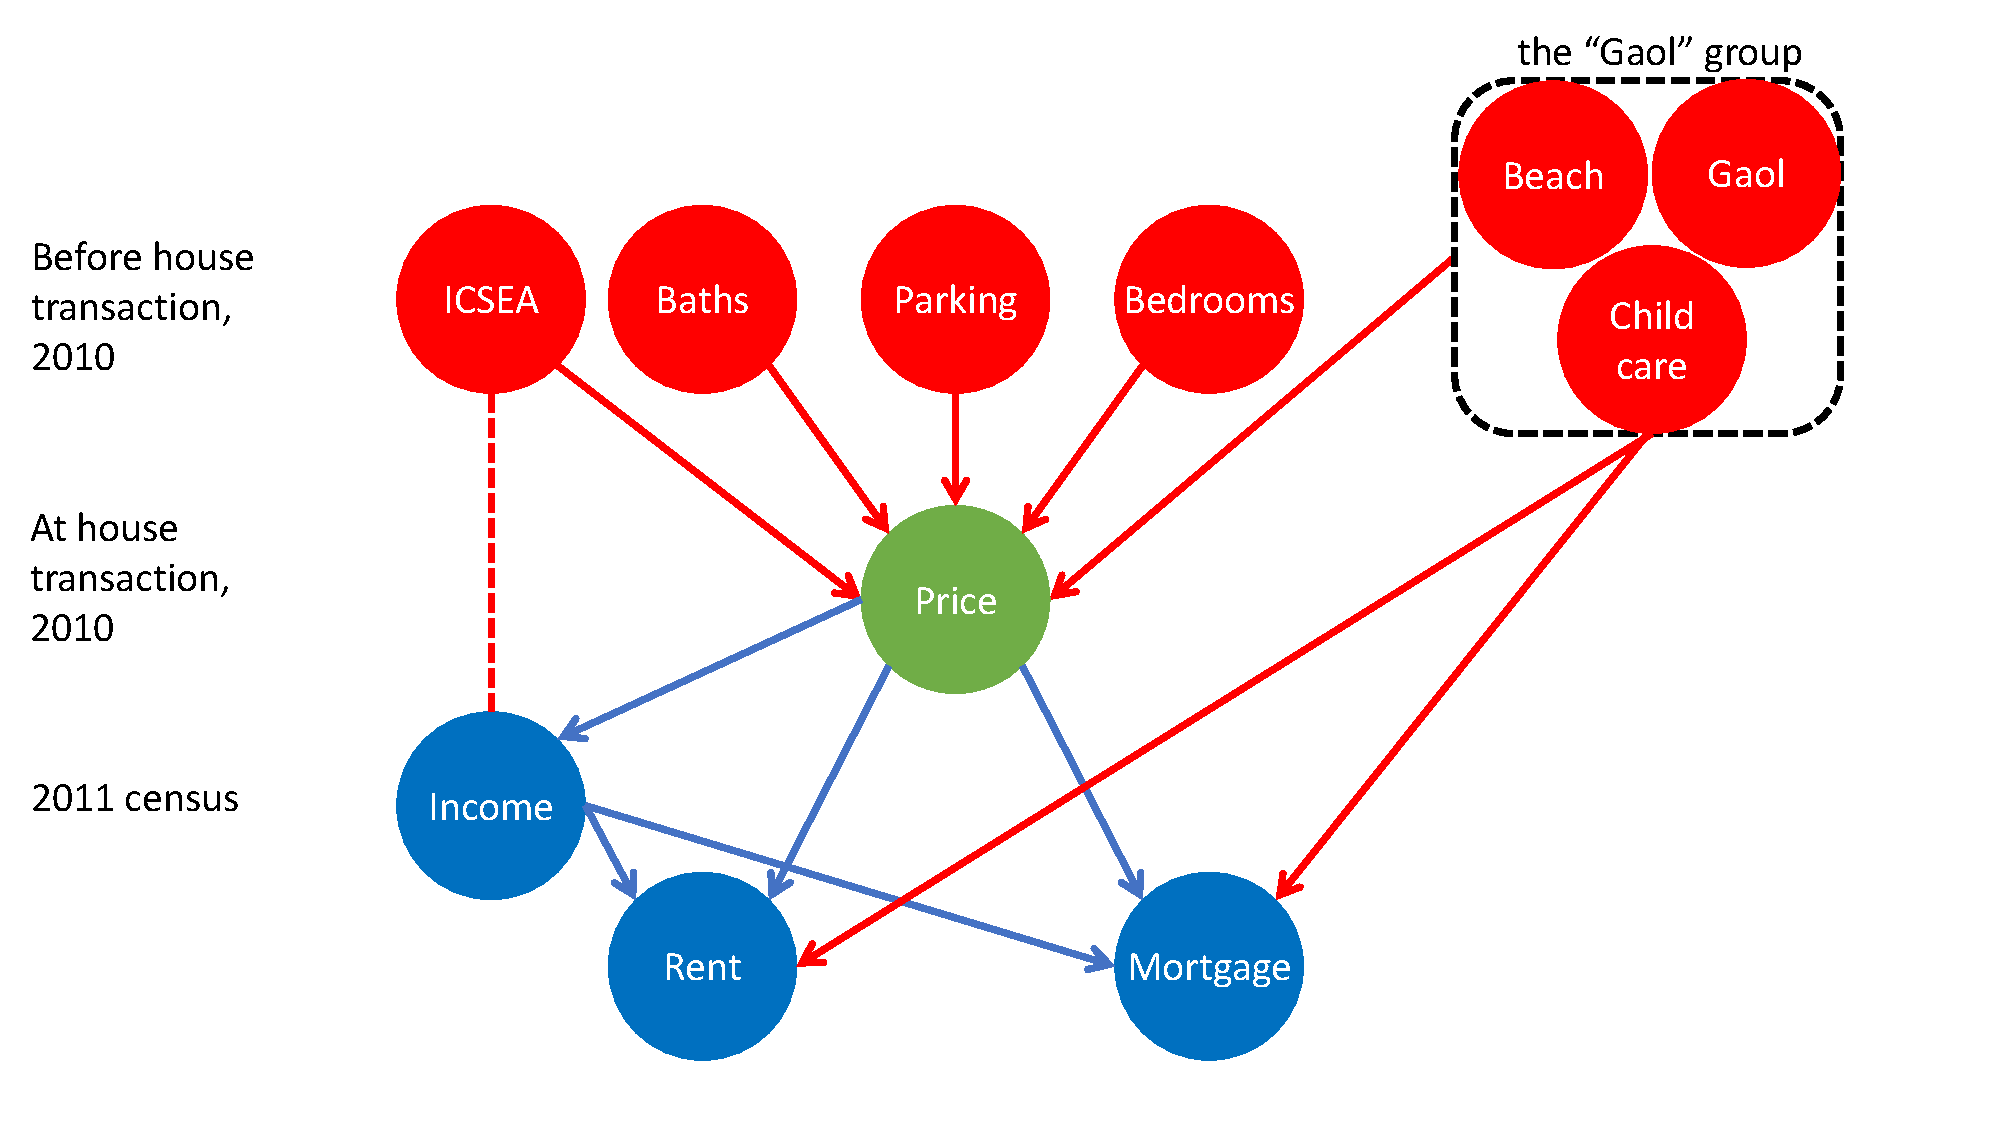
\includegraphics[width=0.6\paperwidth]{BN_post.pdf}
  %
  \caption{The estimated graph based on solar variable selection.}
  %
  \label{fig:BN_post}
  %
\end{figure}

\subsection{Estimation of the Backdoor Effect}

Figure~\ref{fig:BN_post} shows that a parent of price can indirectly cause a change in rent or mortgage through price (e.g., $\mathrm{Bath} \rightarrow \mathrm{Price} \rightarrow \mathrm{Mortgage}$), confirming the existence of the frontdoor effect(FE). The last step of graph learning is to determine whether the parents of price can cause a change in rent or mortgage without going through price. Such a causal effect is referred to as a backdoor effect (BE) and is illustrated by black arrows in Figure~\ref{fig:Backdoor_bath}.

A BE could appear either as in Figure~\ref{fig:Backdoor_bath2} or as in Figure~\ref{fig:Backdoor_bath3}. In Figure~\ref{fig:Backdoor_bath2}, Baths cause a change in Mortgage after controlling for price even. It is difficult to control for BEs of this kind absent infinitely large data. By contrast, the BE in Figure~\ref{fig:Backdoor_bath3} is controlled by Price and the `?' variable(s), because Baths do not cause any further change in Mortgage. We can estimate which causal structure fits the data better as follows. First, we find out which of Figures~\ref{fig:Backdoor_bath1} and \ref{fig:Backdoor_bath2} fits the data better without controlling for any other variables. If Figure~\ref{fig:Backdoor_bath1} is chosen, it implies that there is no BE. If Figure~\ref{fig:Backdoor_bath2} is chosen, there exists a BE and we need to combinatorially determine whether there exists a variable(s) `?' in the BE from Baths to Mortgage.

\begin{figure}[H]
  %
  \centering
  %
  \subfloat[\label{fig:Backdoor_bath1} subgraph without BE]
  {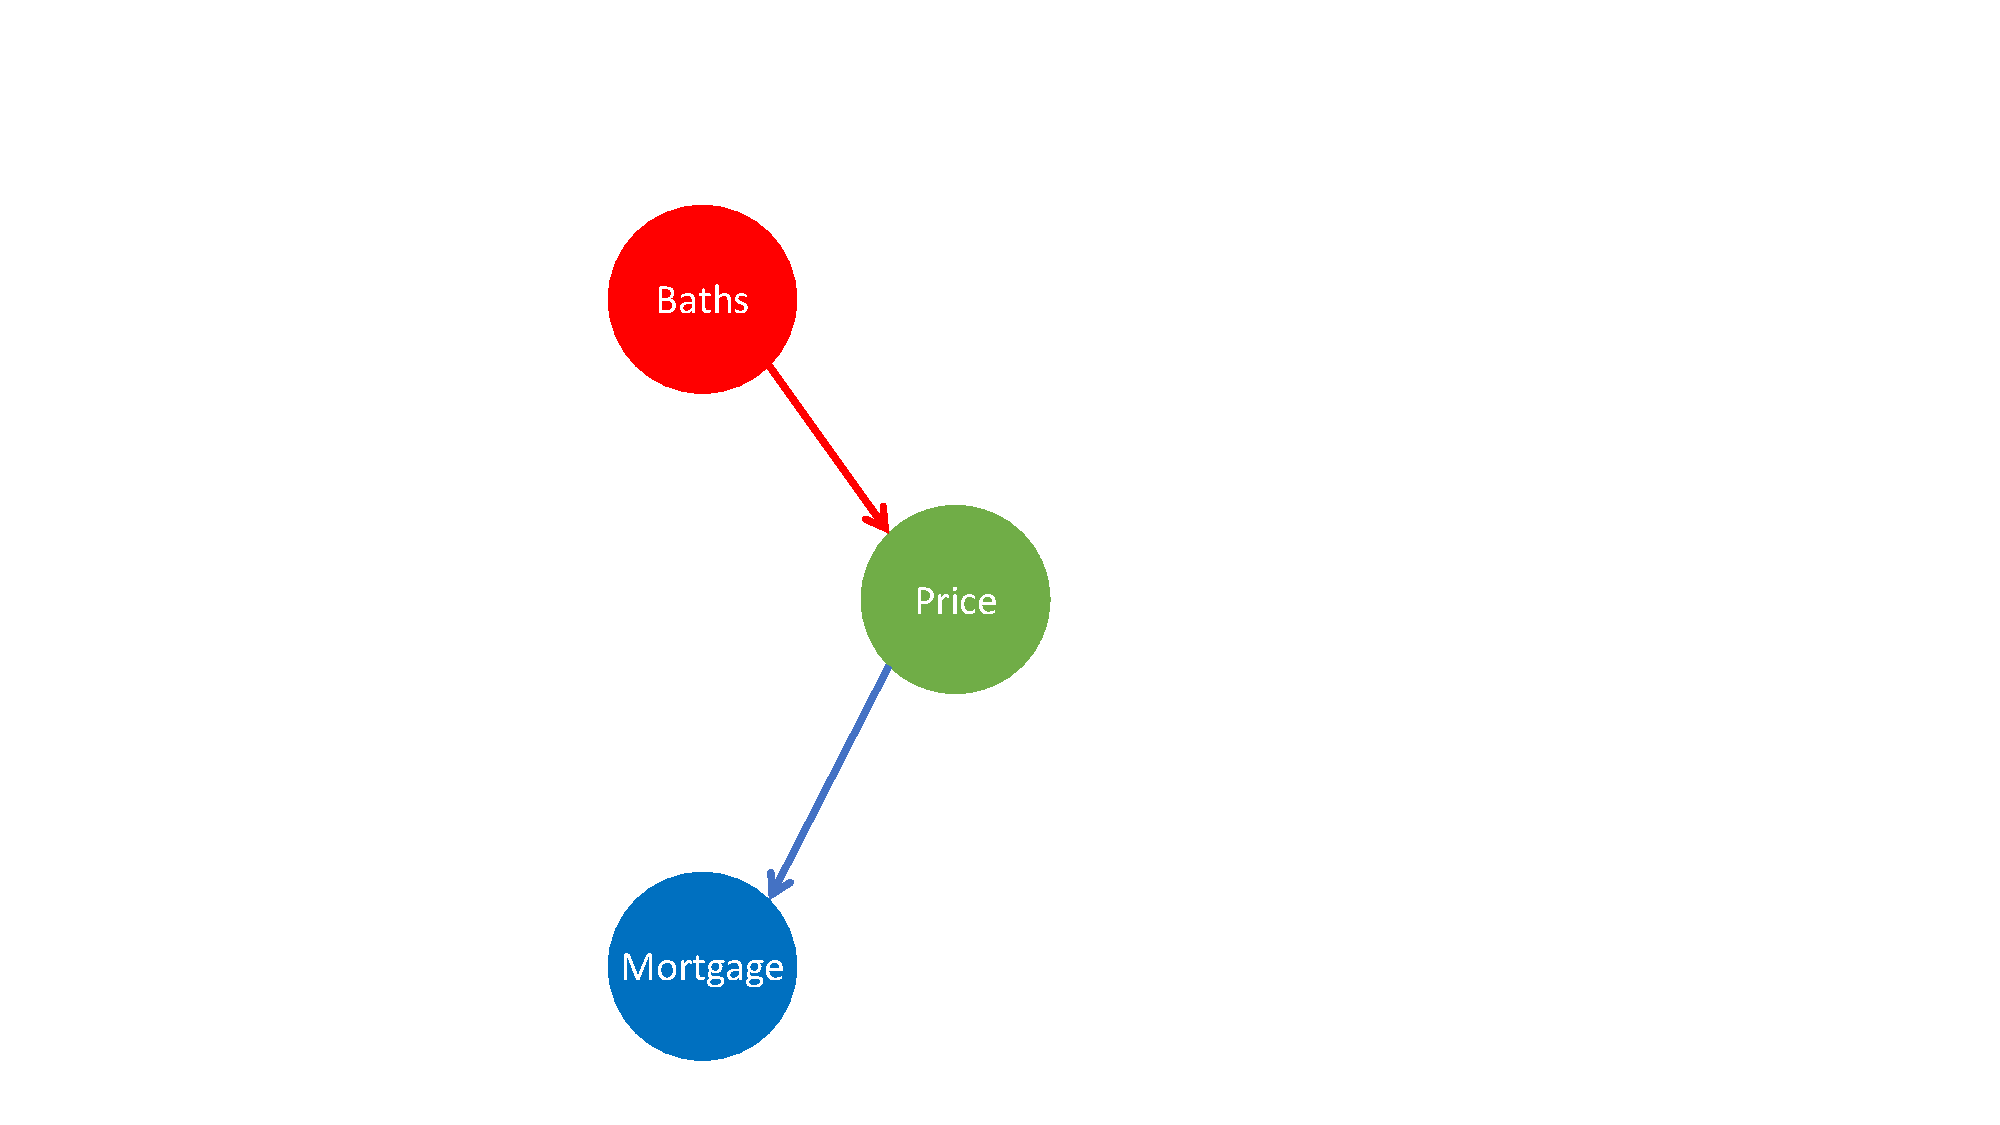
\includegraphics[width=0.18\paperwidth]{Backdoor_bath1.pdf}}
  \hfil
  \subfloat[\label{fig:Backdoor_bath2} subgraph with BE]
  {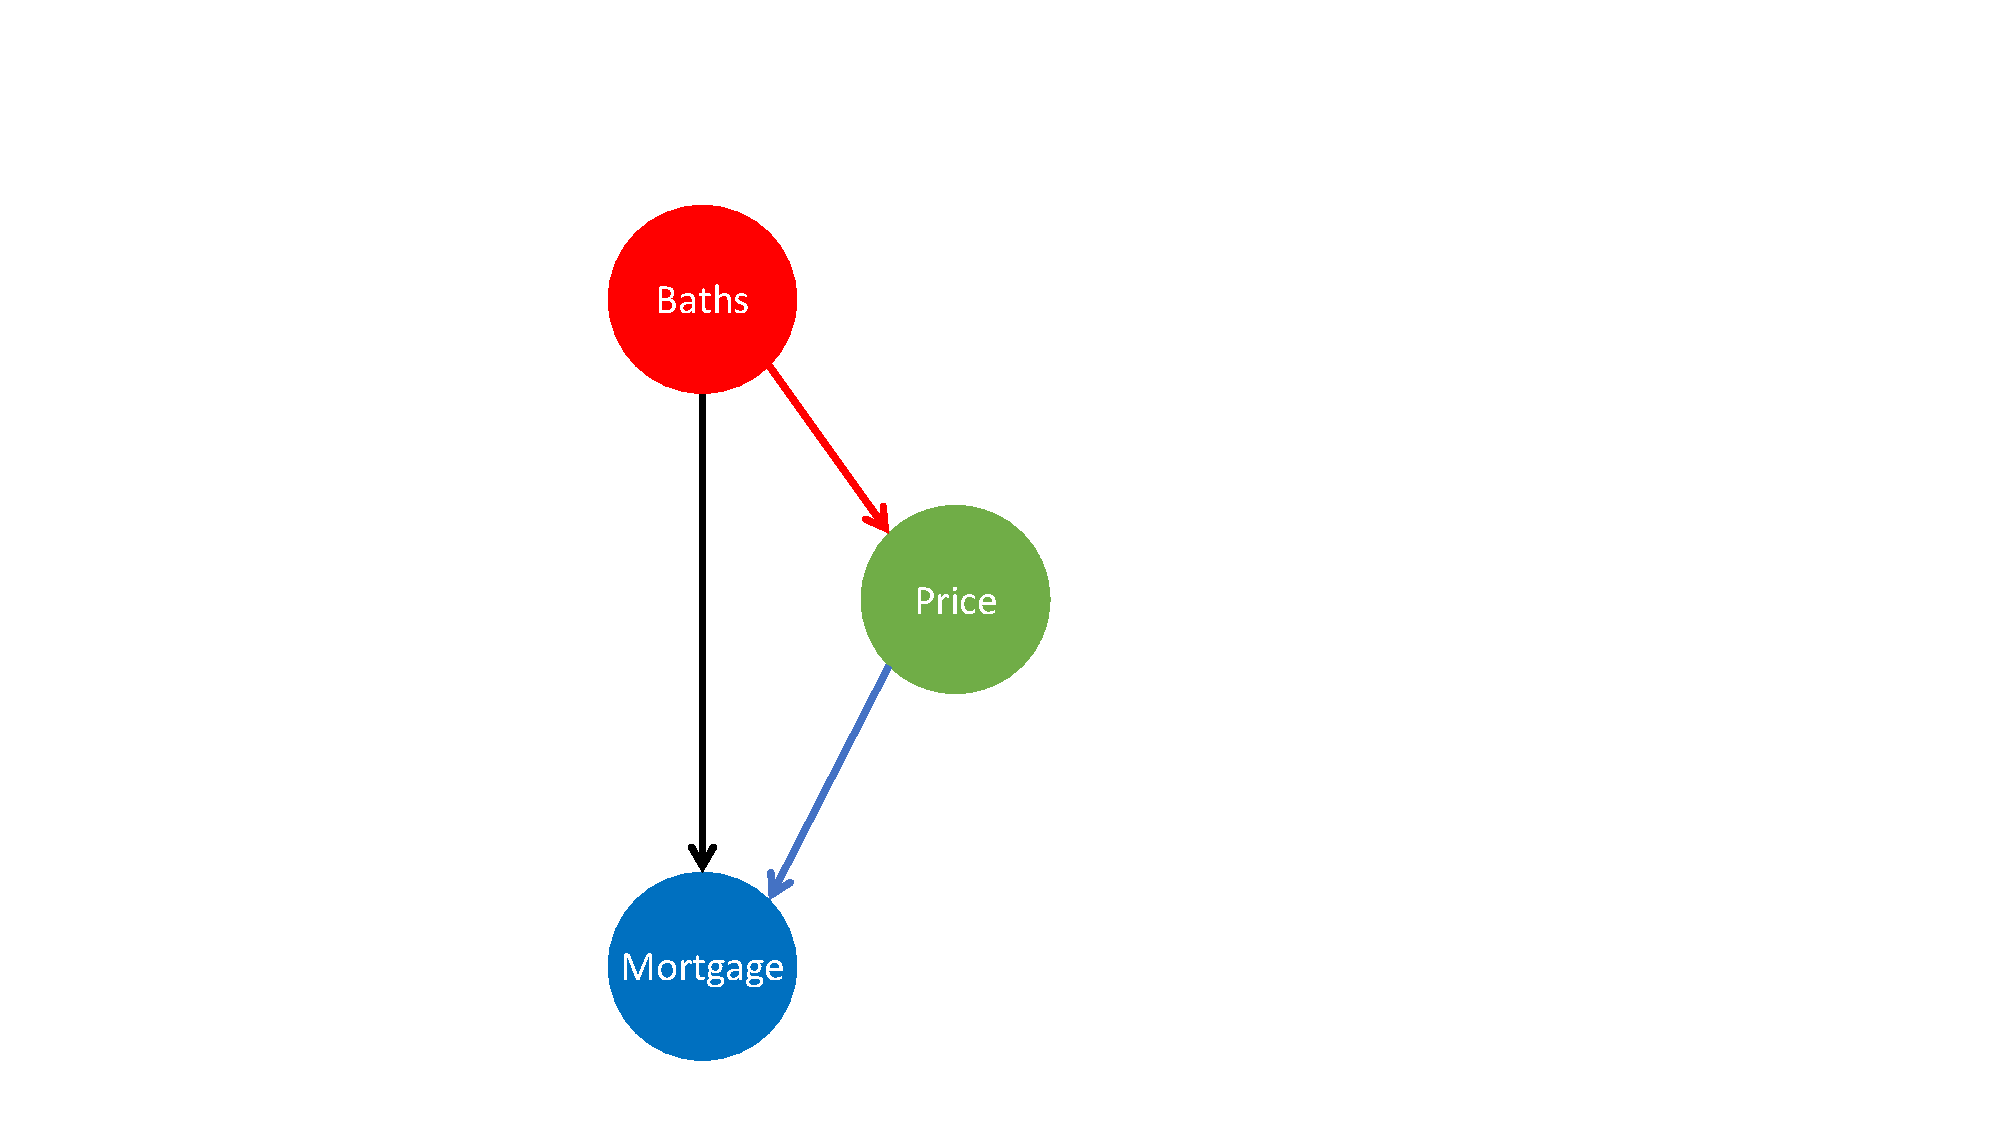
\includegraphics[width=0.18\paperwidth]{Backdoor_bath2.pdf}}
  \hfil
  \subfloat[\label{fig:Backdoor_bath3} alternative subgraph with BE]
  {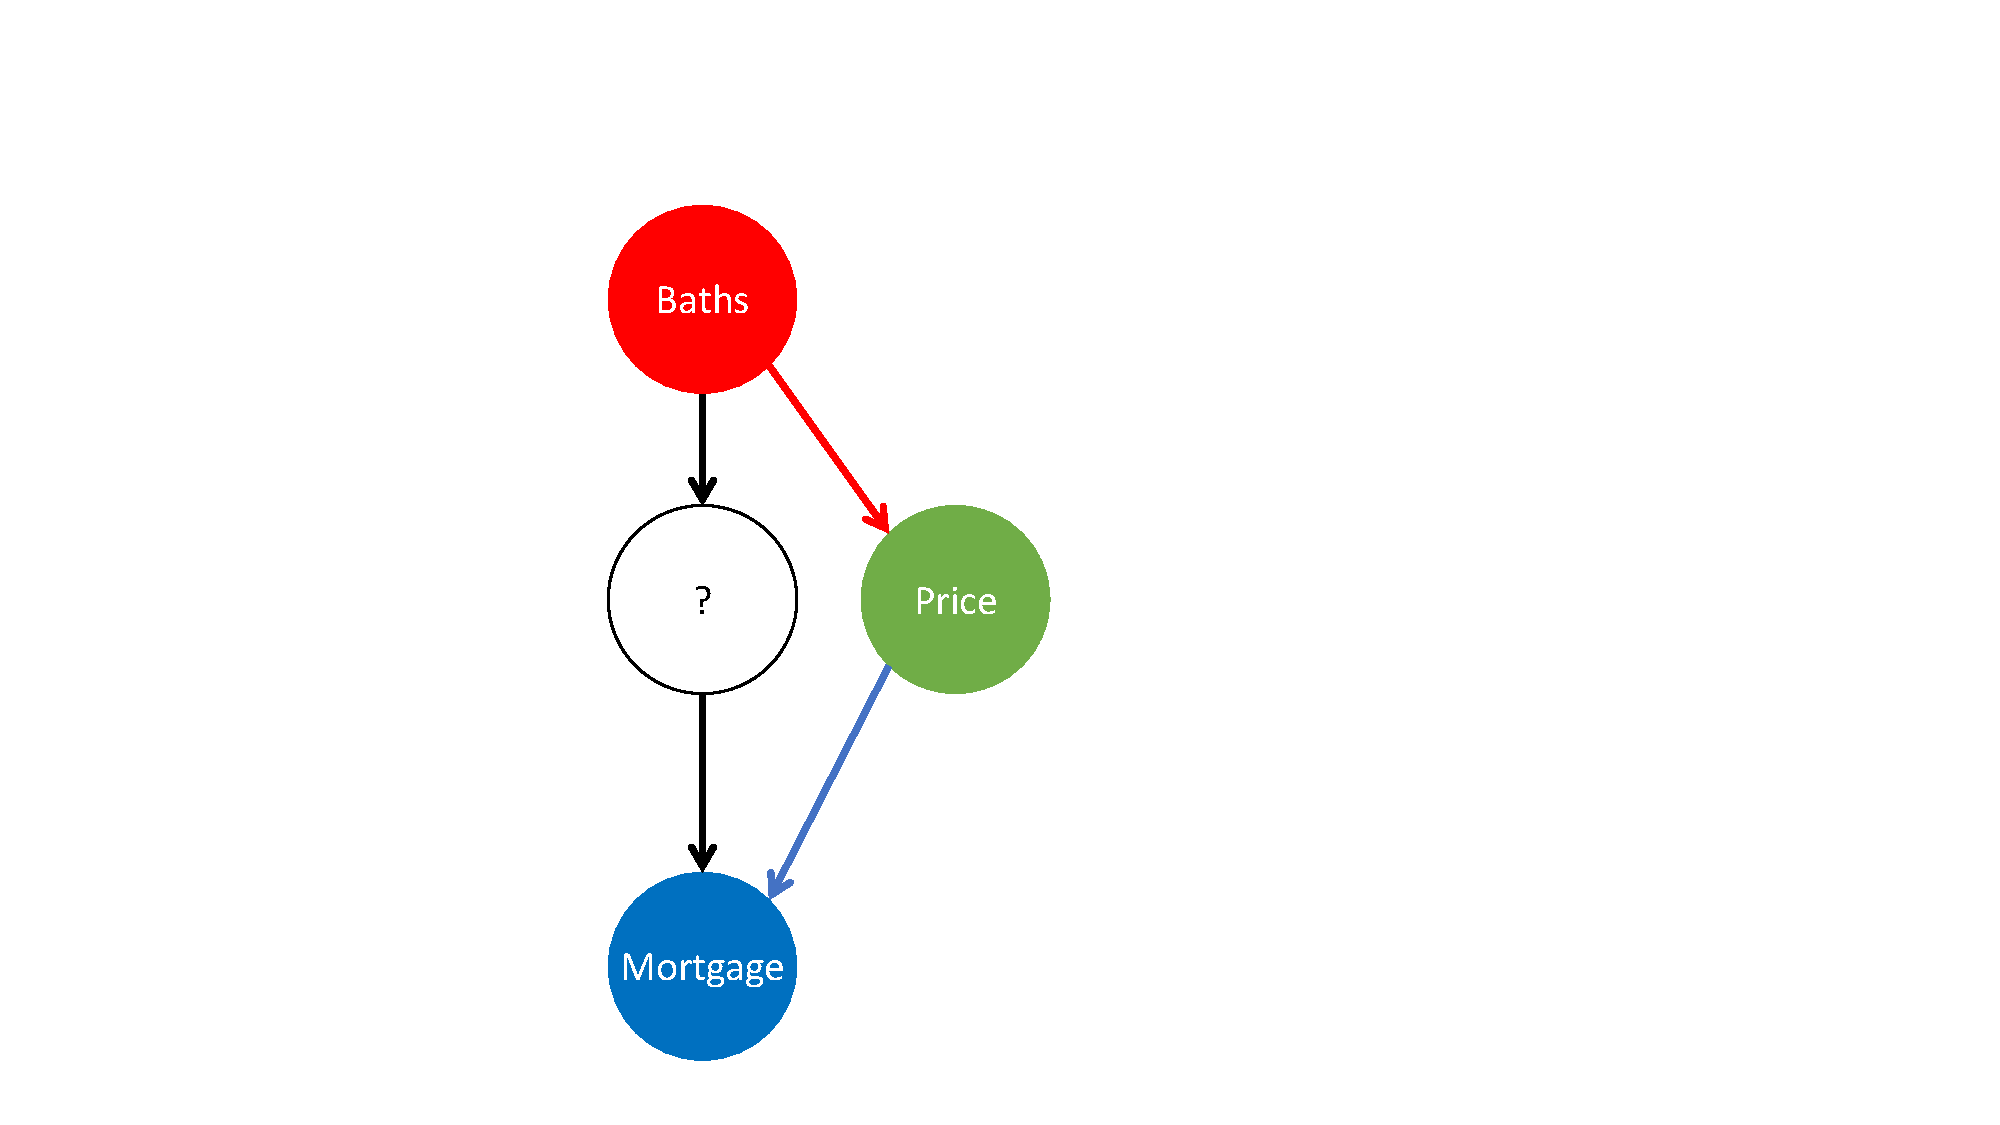
\includegraphics[width=0.18\paperwidth]{Backdoor_bath3.pdf}}
  %
  \caption{Illustration of BE estimation between baths, price and mortgage.}
  \label{fig:Backdoor_bath}
  %
\end{figure}

We use the score-based learning method to find the optimal causal structure. Specifically, we estimate the AIC, BIC, and BGE scores of Figure~\ref{fig:Backdoor_bath1} (column `No BE' in Table~\ref{Table:Backdoor}) and Figure~\ref{fig:Backdoor_bath2} (column `BE' in Table~\ref{Table:Backdoor}) and choose the one with the lowest score. If bath only causes mortgage via price, the conditional correlation between baths and mortgage will be very close to zero holding price constant. Hence, due to the overfitting of the causal structure in Figure~\ref{fig:Backdoor_bath2}, its AIC, BIC, or BGE scores will be higher than for Figure~\ref{fig:Backdoor_bath1}, implying that the no-BE graph fits the data better. By replacing baths with parking or bedrooms in Figure~\ref{fig:Backdoor_bath}, we can instead check whether a BE exists between mortgage and other parents of price. In a similar vein, by replacing mortgage with rent, we can also check whether a BE exists between rent and any parent of price.

\begin{table}[H]
  %
  \renewcommand*{\arraystretch}{0.8}
  \small
  \centering
  \caption{Estimation of the BE for price (optimal AIC, BIC, and BGE scores in red)}
  %
  \label{Table:Backdoor}
  %
  \begin{tabular}{cll>{\color{red}}ll>{\color{red}}l}
    %
    \toprule
    & & \multicolumn{2}{c}{logRent} & \multicolumn{2}{c}{logMortgage} \\
    \cmidrule(lr){3-4} \cmidrule(lr){5-6}
    %
    & & \multicolumn{1}{c}{BE} & \multicolumn{1}{c}{No BE}
      & \multicolumn{1}{c}{BE} & \multicolumn{1}{c}{No BE} \\
    %
    \midrule
             & AIC & $-$23726.55 & $-$23731.28 & $-$19437.42 & $-$19482.37 \\
    Baths    & BIC & $-$23759.74 & $-$23760.78 & $-$19470.61 & $-$19511.87 \\
             & BGE & $-$23758.70 & $-$23760.01 & $-$19470.54 & $-$19512.35 \\
    \cmidrule{1-6}
             & AIC & $-$27197.09 & $-$27500.08 & $-$23060.65 & $-$23251.17 \\
    Bedrooms & BIC & $-$27230.27 & $-$27529.58 & $-$23093.84 & $-$23280.67 \\
             & BGE & $-$27230.75 & $-$27529.87 & $-$23095.31 & $-$23282.22 \\
    \cmidrule{1-6}
             & AIC & $-$25002.25 & $-$25064.54 & $-$20762.16 & $-$20815.63 \\
    Parking  & BIC & $-$25035.44 & $-$25094.04 & $-$20795.35 & $-$20845.13 \\
             & BGE & $-$25034.62 & $-$25093.35 & $-$20795.46 & $-$20845.70 \\
  \bottomrule
  %
  \end{tabular}
  %
\end{table}

Table~\ref{Table:Backdoor} shows the results from BE estimation. We use logRent and logMortgage for BE estimation because, while the score-based learning method works well on many subgaussian variables for small $p/n$, the distributions of rent and mortgage are right-skewed. The log transform can significantly reduce right skewness and improve the accuracy of the AIC, BIC, and BGE scores. Table~\ref{Table:Backdoor} clearly shows that the graphs without BEs consistently have lower AIC, BIC, and BGE scores, confirming that there is no BE. As a result, Figure~\ref{fig:BN_post} is the final estimated graph for the MB of price; there is no need to add a BE.

We ignore ICSEA, income, and the gaol group in Table~\ref{Table:Backdoor} for statistical reasons. Due to violation of the IRC in the gaol group, it is difficult to estimate accurately any BEs variables in the group may have on the children of price.\footnote{Statistically, the minimal eigenvalue of the covariance matrix may be very close to $0$, resulting in unreliable AIC, BIC, or BGE scores.} ICSEA is constructed (by ACARA) from a number of variables such as household income, family wealth, and other measures of the household socio-economic status. As a result, there may exist complicated causal relations between the determinants of ICSEA and price, which we cannot investigate because we do not know precisely how ICSEA is constructed.

\subsection{Graph interpretation and remarks on AreaSize}

Figure~\ref{fig:BN_post} is consistent with economic intuition about the dynamics of the house market. First, houses with more desirable features and better locations are purchased by higher-income households at higher prices. Second, higher house prices causes higher mortgage repayments and higher rental payments. Third, higher-rent houses are leased to higher-income households (households with high ICSEA scores). From a demographic perspective, after higher-income home owners or tenants move into the newly purchased or leased houses, the average income and family income in the local SA1 also increases, reflected on the graph as price causing income.

\begin{figure}[H]
  %
  \centering
  %
  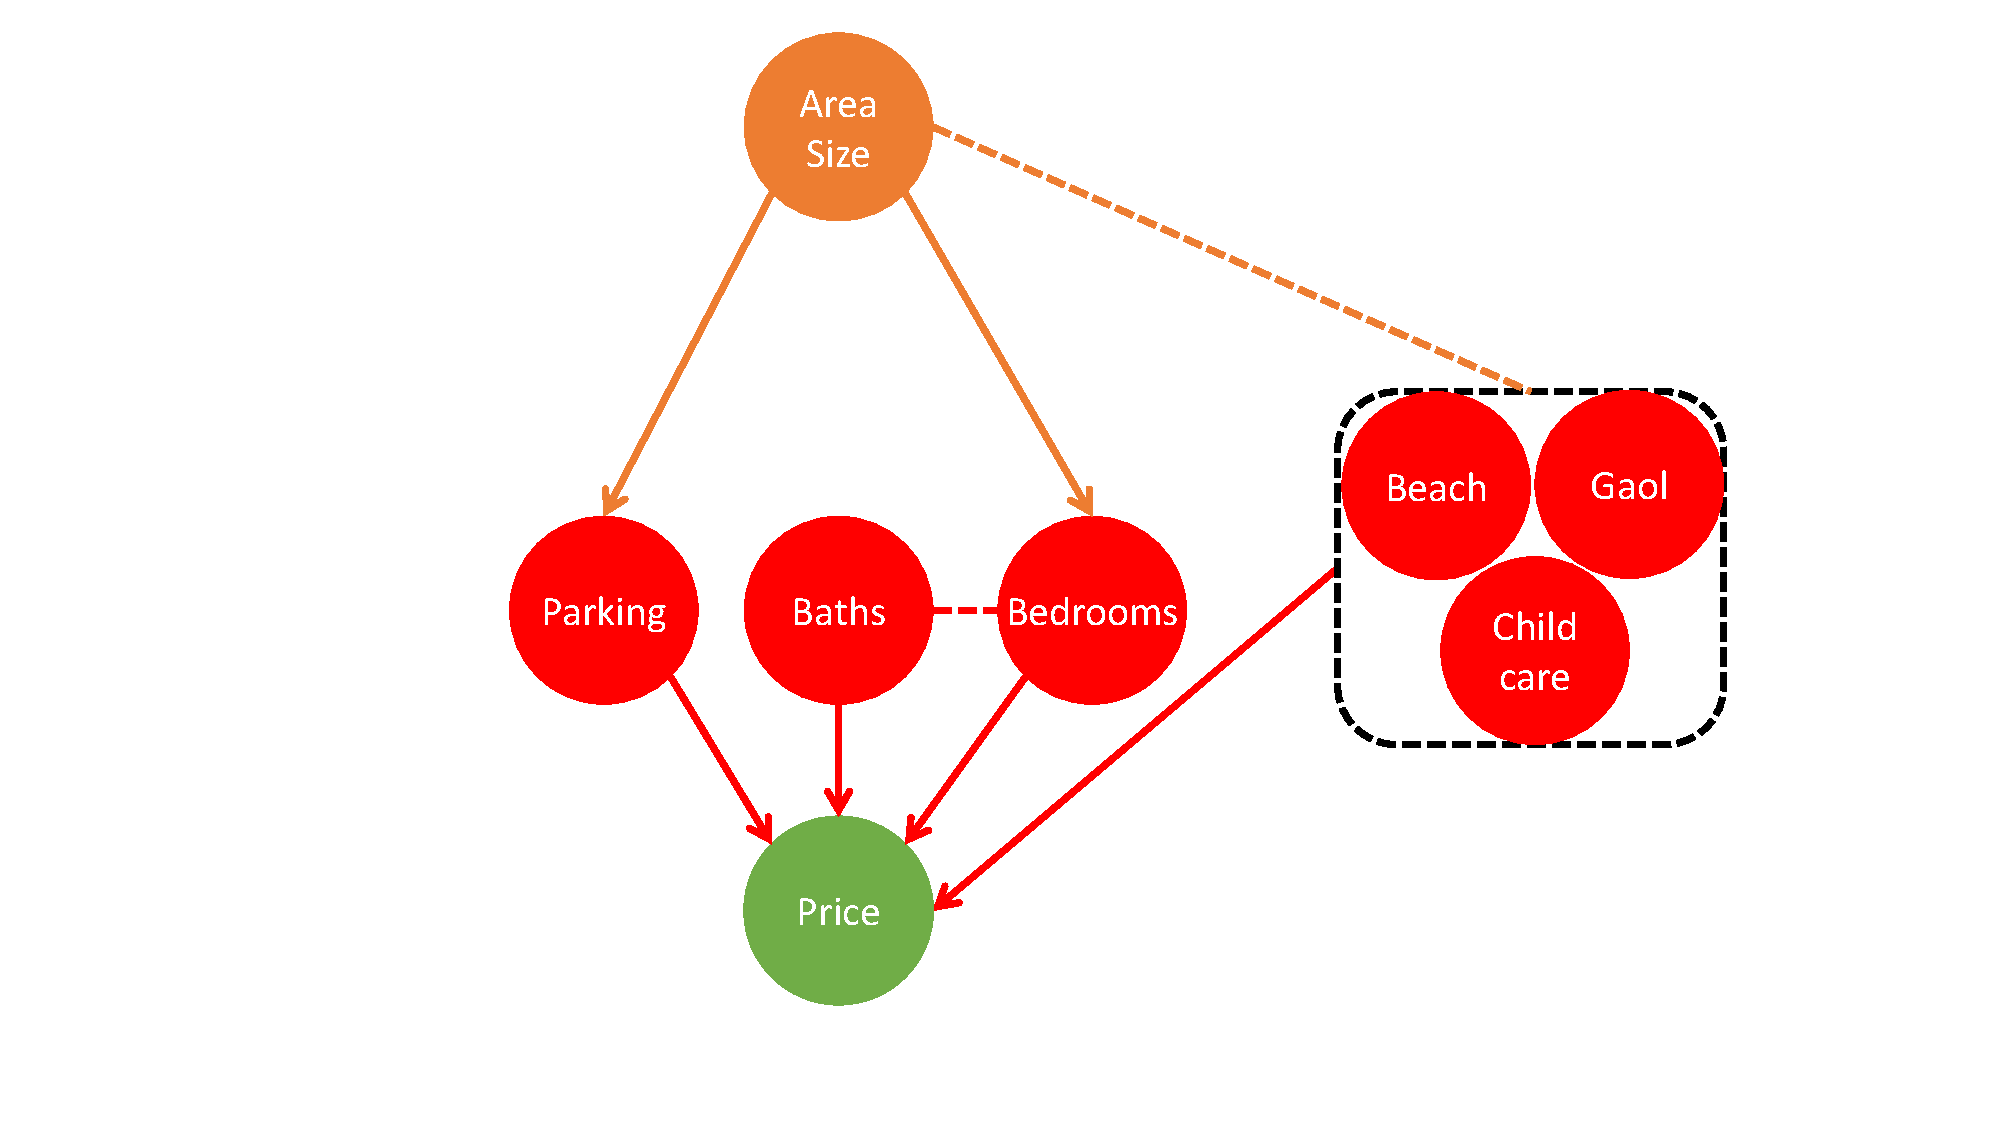
\includegraphics[width=0.45\paperwidth]{AreaSize.pdf}
  %
  \caption{The relation between AreaSize and the parents of price.}
  %
  \label{fig:area_size}
  %
\end{figure}

Surprisingly, land size (AreaSize) is not selected into the MB of price, which seems counterintuitive. However, this can be explained using Figure~\ref{fig:area_size}. Firstly, the land sizes of houses in different locations are not comparable. A downtown terrace house with small land size can be more expensive than a house on a large plot 10km from downtown. Hence, ceteris paribus, AreaSize would have much more explanatory power on price if we compared houses within a local area or spatial neighbourhood, which requires a spatial statistics technique as opposed to simply controlling for distance to various locations.\footnote{For example, lasso variable selection within a spatial Gaussian kernel.} Secondly, land size is originally determined when the land was subdivided, which precedes house construction. Thus, AreaSize also constraints the construction of parking spaces, bathrooms, bedrooms, and so on. In terms of the graph, AreaSize is likely a parent of parking and bedrooms and may also be simultaneously determined with location when the land is subdivided. Thus, AreaSize is not part of the MB of price.

It is also interesting to note that, unlike parking and bedrooms, the number of bathrooms is not a child of AreaSize and that there is a undirected edge between baths and bedrooms. This finding is data-driven: $\mathrm{corr} \left( \mathrm{Bath}, \mathrm{AreaSize} \right) \approx 0$ while $\mathrm{corr} \left( \mathrm{Bath}, \mathrm{bedrooms} \right)$ is significantly nonzero in the data. This phenomenon is not unexpected. During house design and construction, the number of bathrooms is typically a function of the number of bedrooms (essentially, of expected household size). Given household size and number of bedrooms, there seems to be little incentive to build more bathrooms with more AreaSize. At the end of the day, due to a lack of data on the first-hand house market and new construction, we are unable to infer a graph incorporating construction and land purchase and will not pursue the topic further.

\section{Endogeneity detection and instrument selection \label{section:application}}

With the estimated graph in hand, we can begin the instrument selection procedure using Definition~\ref{def:instrument_variable}. The first step to selecting a valid instrument is to ensure there is endogeneity in the graph, otherwise we only waste degrees of freedom.

\subsection{Endogeneity detection using graphs}

Price is endogenous statistically and empirically. Figure~\ref{fig:BN_post} depicts a graph that reflects a statistically dynamic system. The input of the system is the gaol group, house attributes, and ICSEA; rent and mortgage are two outputs, and price is internally determined by the system. As a result, price is highly likely to be endogenous. The endogeneity of price is also supported statistically by the variable selection results. For example, by estimating linear and log solar regressions of rent on all the other selected variables, we have the following estimated regression models.
%
\begin{align}
 %
  \mathrm{logRent} = \alpha_0 & + \alpha_1 \cdot \mathrm{TotPop} + \alpha_2 \cdot \mathrm{Household\_size} + \alpha_3 \cdot \mathrm{Beach} + \alpha_4 \cdot \mathrm{ChildCare} \notag  \\
  & + \alpha_5 \cdot \mathrm{Gaol} + \alpha_6 \cdot \mathrm{PrimaryHigh}  + \alpha_7 \cdot \mathrm{ICSEA} + \alpha_8 \cdot \mathrm{logPersonInc} \notag   \\
  & + \alpha_9 \cdot \mathrm{logFamInc} + \alpha_{10} \cdot \mathrm{logPrice} + u, \label{OLS:solar_logRent} \\
  %
  \mathrm{Rent} = \gamma_0 & + \gamma_1 \cdot \mathrm {Household\_size} + \gamma_2 \cdot \mathrm{Beach} + \gamma_3 \cdot \mathrm{ChildCare} + \gamma_4 \cdot \mathrm{Gaol} \notag \\
  & + \gamma_5 \cdot \mathrm{PrimaryHigh} + \gamma_6 \cdot \mathrm{Mortgage} + \gamma_7 \cdot \mathrm{ICSEA} + \gamma_8 \cdot \mathrm{FamInc} \notag \\
  & + \gamma_9 \cdot \mathrm{PersonInc} + \gamma_{10} \cdot \mathrm{Price} + u. \label{OLS:solar_Rent}
  %
\end{align}
%
Since the $p/n$ ratio is almost $1/200$, the solar variable selection results are statistically robust and accurate. Solar includes log(price) and price in (\ref{OLS:solar_logRent}) and (\ref{OLS:solar_Rent}), respectively, implying that price is an important covariate in the rent regressions and that it is highly likely that rent and price are simultaneously determined. Thus, along with the solar variable selection results in (\ref{OLS:solar}) and (\ref{OLS:solar_log}), we can establish the simultaneous equations models in log terms:
%
\begin{equation}
  %
  \begin{cases}
    %
    \mathrm{logRent} = \alpha_0 & + \alpha_1 \cdot \mathrm{TotPop} + \alpha_2 \cdot \mathrm{Household\_size} + \alpha_3 \cdot \mathrm{Beach} + \alpha_4 \cdot \mathrm{ChildCare} \\
    & + \alpha_5 \cdot \mathrm{Gaol} + \alpha_6 \cdot \mathrm{PrimaryHigh}  + \alpha_7 \cdot \mathrm{ICSEA} + \alpha_8 \cdot \mathrm{logPersonInc} \\
    & + \alpha_9 \cdot \mathrm{logFamInc} + \alpha_{10} \cdot \mathrm{logPrice} + u_1, \\
    %
    \mathrm{logPrice} = \beta_0 & + \beta_1 \cdot \mathrm{logMortgage} + \beta_2 \cdot \mathrm{logRent} + \beta_3 \cdot \mathrm{logFamInc} + \beta_4 \cdot \mathrm{Bedrooms} \\
    & + \beta_5 \cdot \mathrm{Baths} + \beta_6 \cdot \mathrm{Parking} + \beta_7 \cdot \mathrm{Beach} + \beta_8 \cdot \mathrm{Gaol} + \beta_9 \cdot \mathrm{ICSEA} + u_2;
    %
  \end{cases}
  %
\label{eqn:SEM_linear}
%
\end{equation}
%
or in linear terms
%
\begin{equation}
  %
  \begin{cases}
    %
    \mathrm{Rent} = \gamma_0 & + \gamma_1 \cdot \mathrm {Household\_size} + \gamma_2 \cdot \mathrm{Beach} + \gamma_3 \cdot \mathrm{ChildCare} + \gamma_4 \cdot \mathrm{Gaol} \\
    & + \gamma_5 \cdot \mathrm{PrimaryHigh} + \gamma_6 \cdot \mathrm{Mortgage} + \gamma_7 \cdot \mathrm{ICSEA} + \gamma_8 \cdot \mathrm{FamInc} \\
    & + \gamma_9 \cdot \mathrm{PersonInc} + \gamma_{10} \cdot \mathrm{Price} + u_1, \\
    %
    \mathrm{Price} = \delta_0 & + \delta_1 \cdot \mathrm{Mortgage} + \delta_2 \cdot \mathrm{Rent} +
    \delta_3 \cdot \mathrm{FamInc} + \delta_4 \cdot \mathrm{Bedrooms} \\
    & + \delta_5 \cdot \mathrm{Baths} + \delta_6 \cdot \mathrm{Parking} + \delta_7 \cdot \mathrm{Beach} + \delta_8 \cdot \mathrm{Gaol} + \delta_9 \cdot \mathrm{ICSEA} + u.
    %
  \end{cases}
  %
  \label{eqn:SEM_log}
  %
\end{equation}

The simultaneous determination of rent, price, and mortgage is also empirically intuitive. Before bidding on a house, the buyer needs to estimate the upper bound of the mortgage a bank will offer or, if the purchase is for investment purposes, how much rent the property will return. Before a bank decides on a mortgage application, it typically requests a valuation of the house price and the expected rent. Similarly, rent is typically related to the price of house and monthly mortgage amount.\footnote{In a competitive market with certainty and zero transactions costs, of course, rent would exactly cover the mortgage, which itself would be equal to the price of the house.}

\subsection{Instrument selection using graphs}

We focus on the regression analysis of rent in this paper, but the mortgage analysis proceeds along the same lines. Given price is endogenous, we need to find a valid instrument in the rent regression. A valid instrument must satisfy Definition~\ref{def:instrument_variable} and non-existence of a BE (Figures~\ref{fig:instrument} and \ref{fig:not_instrument1}).

From Figure~\ref{fig:BN_post}, we directly uncover 3 instrumental variables: baths, bedrooms, and parking, all of which satisfy Definition~\ref{def:instrument_variable} only if we control the Gaol group variables. As shown in Figure~\ref{fig:BE_house}, failing to control for the Gaol group will induce a backdoor effect between rent and any of \{baths, bedrooms, parking\}. Baths, for example, will be unconditionally correlated to Bedrooms, which is unconditionally correlated to the Gaol group due to the confounder AreaSize. Since the Gaol group variables represent house location, they are causally related to rent, creating a BE. The BE violates Definition~\ref{def:instrument_variable} by allowing a change in baths to affect rent while controlling for house price. Thus, baths cannot be an instrument for the causal effect of price on rent because it represents two effects: the causal effect from price to rent and the BE. Hence, it is necessary to control for the Gaol group variables, meaning that they must be included in the instrumental variable regression for rent.

\begin{figure}[H]
  %
  \centering
  %
  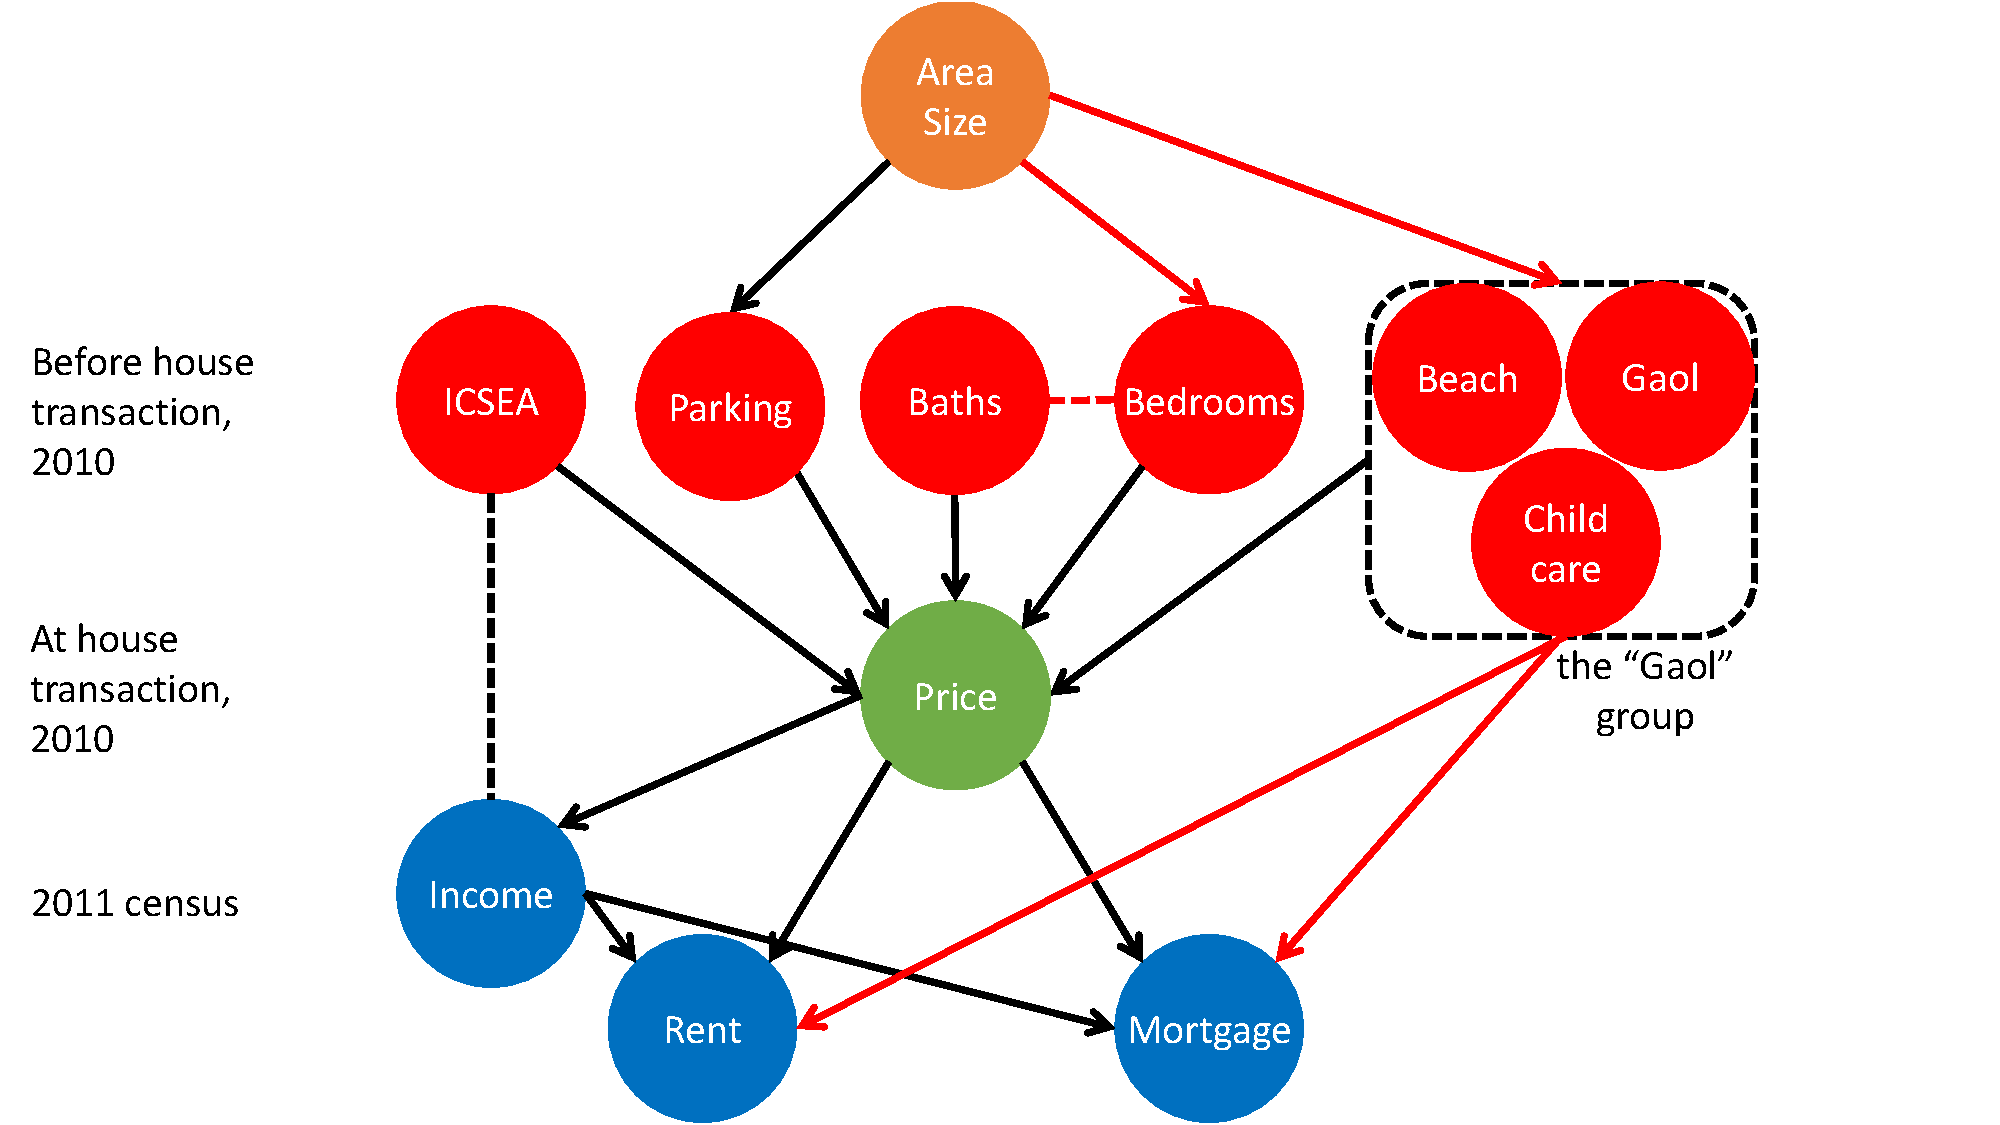
\includegraphics[width=0.5\paperwidth]{BE_house.pdf}
  %
  \caption{Backdoor effect from Bath to Rent (highlighted in red).}
  %
  \label{fig:BE_house}
  %
\end{figure}

Controlling for the Gaol group variables, Figure~\ref{fig:Backdoor_bath} and Table~\ref{Table:Backdoor} confirm that baths, bedrooms, and parking can only affect rent through price, which satisfies G2 in Definition~\ref{def:instrument_variable}. Yet these two conditions are for a general statistical dynamic system. The score-based learning method only requires a subgaussian distribution for each variable, which permits any form of nonlinear causation among variables.\footnote{For nonlinear graph estimation with endogeneity bias correction, we need dependence measures such as mutual information and the Hilbert-Schmidt independence criterion, both of which would impose enormous computation loads in our high-dimensional database. Hence, we skip this topic in this paper.} However, classic endogeneity analysis in regression requires linearity among all the variables. To ensure the 3 variables fit a system of linear regression equations, we need to check the correlation between rent and the instrument for price, shown in Table~\ref{table:iv_correlation}.

\begin{table}[H]
  %
  \renewcommand*{\arraystretch}{0.8}
  \small
  \centering
  \caption{Correlation table for the instruments, price, and rent}
  %
  \label{table:iv_correlation}
  %
  \begin{tabular}{l.....}
    %
    \toprule
      & \multicolumn{1}{c}{Baths} & \multicolumn{1}{c}{Parking} & \multicolumn{1}{c}{Bedroom}
      & \multicolumn{1}{c}{Price} & \multicolumn{1}{c}{logPrice} \\
    %
    \midrule
        Rent     & 0.19  & 0.069   & 0.061   & 0.34  &          \\
        logRent  & 0.16  & 0.043   & 0.023   &       & 0.32     \\
        Price    & 0.52  & 0.34    & 0.46    &       &          \\
        logPrice & 0.57  & 0.41    & 0.60    &       &          \\
    \bottomrule
    %
  \end{tabular}
  %
\end{table}

Table~\ref{table:iv_correlation} clearly shows that bedrooms and parking do not fit the linear system as instruments for price: $\mathrm{corr} \left( \mathrm{logRent}, \mathrm{Parking} \right)$ and $\mathrm{corr} \left( \mathrm{logRent}, \mathrm{bedrooms} \right)$ are too weak. As a result, even though the correlations between these variables and logPrice are quite high, the predicted value of logPrice using these two variables will not be able to explain enough of the variation in logRent using 2SLS or other IV regressions. Moreover, the weak instruments may lead to incorrect coefficient signs and values leading to mistakes in interpretation. These concerns are confirmed in Tables~\ref{table:IV_2LSL_log} and \ref{table:IV_2LSL_linear}.

\begin{table}[H]
  %
  \renewcommand*{\arraystretch}{0.8}
  \centering
  \caption{logRent regressions: 2SLS coefficients and t-values}
  \label{table:IV_2LSL_log}
  %
  \resizebox*{!}{1.0\textwidth}{%
  \begin{tabular}{r....}
    %
    \toprule
     & \multicolumn{1}{c}{OLS} & \multicolumn{3}{c}{2SLS} \\
     \cmidrule{3-5}
     & & \multicolumn{1}{c}{Baths}
       & \multicolumn{1}{c}{Bedrooms}
       & \multicolumn{1}{c}{Parking} \\
    %
    \midrule
    const           & 1.87     & 1.60       & 2.2169        & 1.91         \\
                    & (17.34)  & (11.10)    & (17.92)       & (11.77)      \\
    TotPop          & 0.0002   & 0.0002     & 0.0002        & 0.0002       \\
                    & (11.31)  & (11.63)    & (10.40)       & (10.84)      \\
    household\_size & 0.31     & 0.29       & 0.32          & 0.31         \\
                    & (27.01)  & (23.60)    & (27.22)       & (23.31)      \\
    Beach           & -2.35    & -2.21      & -2.55         & -2.38        \\
                    & (-14.04) & (-12.65)   & (-14.67)      & (-12.80)     \\
    ChildCare       & -1.67    & -1.57      & -1.81         & -1.69        \\
                    & (-12.31) & (-11.11)   & (-12.90)      & (-11.42)     \\
    Gaol            & 1.23     & 1.19       & 1.28          & 1.24         \\
                    & (7.09)   & (6.82)     & (7.35)        & (7.02)       \\
    PrimaryHigh     & -1.30    & -1.37      & -1.22         & -1.29        \\
                    & (-7.81)  & (-8.13)    & (-7.21)       & (-7.63)      \\
    ICSEA           & 0.0004   & 0.0004     & 0.0005        & 0.0004       \\
                    & (5.81)   & (5.00)     & (6.76)        & (5.77)       \\
    logPersonInc    & 0.50     & 0.51       & 0.49          & 0.50         \\
                    & (17.46)  & (17.66)    & (17.10)       & (17.31)      \\
    logFamInc       & -0.04    & -0.07      & -0.0090       & -0.0409      \\
                    & (-1.84)  & (-2.76)    & (-0.35)       & (-1.49)      \\
    logPrice        & 0.0053   & 0.0410     & -0.0428       & -0.0014      \\
                    & (0.72)   & (2.80)     & (-3.90)       & (-0.07)      \\
    %
    \midrule
    $p$         & & & & \\
    $R^2$       & 0.3650    & 0.3632     & 0.3618        & 0.3649       \\
    $\bar{R}^2$ & 0.3645    & 0.3627     & 0.3612        & 0.3644       \\
    $n$         & 11,796    & 11,796     & 11,796        & 11,796        \\
    \bottomrule
    %
  \end{tabular}}
  %
\end{table}

Table~\ref{table:IV_2LSL_log} shows the 2SLS estimates from the log regressions. Baths, bedrooms, and parking separately as instruments for logPrice. Due to the endogeneity, OLS clearly underestimates the marginal effect of logPrice where it is not significant. In the baths 2SLS, the logPrice coefficient is 7 times larger and the t-value of logPrice is 3 times larger than for the corresponding OLS coefficient, so it is now significant. These results clearly show the bias-correction effect of 2SLS using baths. By contrast, due to the weak correlation between parking, bedrooms, and logRent, both the parking and bedrooms 2SLS move the OLS coefficient of logPrice in the wrong direction, giving the wrong interpretation that higher house prices are associated with lower rent. Also, logPrice in the parking 2SLS is even less significant than in OLS.

\begin{table}[H]
  %
  \renewcommand*{\arraystretch}{0.8}
  \centering
  \caption{Rent regressions: 2SLS coefficients and t-values}
  %
  \label{table:IV_2LSL_linear}
  %
  \resizebox*{!}{1.0\textwidth}{%
  \begin{tabular}{r....}
    %
    \toprule
    %
     & \multicolumn{1}{c}{OLS} & \multicolumn{3}{c}{2SLS} \\
     \cmidrule{3-5}
     & & \multicolumn{1}{c}{Baths}
       & \multicolumn{1}{c}{Bedrooms}
       & \multicolumn{1}{c}{Parking} \\
    %
    \midrule
    %
    const            & -74.336   & -50.537   & -116.40     & -80.687     \\
                     & (-2.2952) & (-1.4809) & (-3.3948)   & (-2.2233)   \\
    household\_size  & 105.60    & 102.56    & 110.95      & 106.40      \\
                     & (25.829)  & (23.629)  & (25.427)    & (23.053)    \\
    Beach            & -841.34   & -795.41   & -922.53     & -853.60     \\
                     & (-12.933) & (-11.478) & (-13.413)   & (-11.477)   \\
    ChildCare        & -574.23   & -549.46   & -618.02     & -580.84     \\
                     & (-10.151) & (-9.3269) & (-10.576)   & (-9.5272)   \\
    Gaol             & 329.80    & 315.15    & 355.71      & 333.72      \\
                     & (4.5646)  & (4.2765)  & (4.8245)    & (4.4669)    \\
    PrimaryHigh      & -331.82   & -343.79   & -310.66     & -328.62     \\
                     & (-4.7021) & (-4.8783) & (-4.3918)   & (-4.6602)   \\
    Mortgage         & 0.0154    & 0.0126    & 0.0203      & 0.0161      \\
                     & (3.4684)  & (2.5347)  & (4.0522)    & (3.0657)    \\
    ICSEA            & 0.0004    & 0.0004    & 0.0005      & 0.0004      \\
                     & (5.8185)  & (5.0046)  & (6.7625)    & (5.7714)    \\
    ICSEA            & 0.0855    & 0.0678    & 0.1169      & 0.0902      \\
                     & (2.9184)  & (2.3028)  & (3.9957)    & (2.9591)    \\
    FamInc           & -0.0012   & -0.0034   & 0.0029      & -0.0006     \\
                     & (-0.1717) & (-0.5222) & (0.4400)    & (-0.0846)   \\
    Inc              & 0.2250    & 0.2276    & 0.2203      & 0.2243      \\
                     & (15.635)  & (15.970)  & (15.410)    & (15.688)    \\
    Price            & 1.95e-05  & 3.04e-05  & 1.98e-07    & 1.66e-05   \\
                     & (3.8921)  & (5.3430)  & (0.0444)    & (2.4782)    \\
    %
    \midrule
    %
    $p$         & & & & \\
    $R^2$       & 0.3462    & 0.3444    & 0.3407      & 0.3461      \\
    $\bar{R}^2$ & 0.3457    & 0.3439    & 0.3401      & 0.3455      \\
    $n$         & 11,974    & 11,974    & 11,974      & 11,974      \\
    %
    \bottomrule
    %
  \end{tabular}}
  %
\end{table}

Table~\ref{table:IV_2LSL_linear} shows the 2SLS results in the linear regressions, which are similar to Table~\ref{table:IV_2LSL_log}. OLS still underestimates the marginal effect of price. The price coefficient in the baths 2SLS is around 50\% larger than the corresponding OLS coefficient. The t-value of price in the baths 2SLS is 40\% larger than the OLS t-value. Similar to Table~\ref{table:IV_2LSL_log}, the parking and bedrooms 2SLS coefficient of price and corresponding marginal effect are even smaller than the corresponding marginal effect in the endogenous OLS.

Finally, to check further the validity of each instrument in 2SLS, we implement four traditional instrument tests and report the results in Table~\ref{table:instrument_test}.

\begin{table}[H]
  %
  \centering
  %
  \caption{Classical tests of instruments in the linear and log regressions}
  %
  \label{table:instrument_test}
  %
\resizebox*{!}{0.45\textwidth}{%
  \begin{tabular}{ll ... ...}
    %
    \toprule
    %
     & & \multicolumn{3}{c}{log} & \multicolumn{3}{c}{linear} \\
     \cmidrule(lr){3-5} \cmidrule(lr){6-8}
    %
     & & \multicolumn{1}{r}{Baths}
       & \multicolumn{1}{r}{Bedrooms}
       & \multicolumn{1}{r}{Parking}
       & \multicolumn{1}{r}{Baths}
       & \multicolumn{1}{r}{Bedrooms}
       & \multicolumn{1}{r}{Parking} \\
    %
    \midrule
    %
    \multirow{2}{*}{\parbox{2.5cm}{Durbin test}}
     & $\chi^2_1$ & 13.0337 & 49.5049 & 0.2538 & 8.8532 & 29.8844 & 0.2795 \\
     & p-value & 0.0003 & 0.0000 & 0.6144 & 0.0029 & 0.0000 & 0.5970 \\
    %
    \midrule
    %
    \multirow{2}{*}{\parbox{2.5cm}{Wu-Hausman test}}
     & $F_{1,11784}$ & 13.0348 & 49.6629 & 0.2535 & 8.8508 & 29.9291 & 0.2793 \\
     & p-value & 0.0003 & 0.0000 & 0.6146 & 0.0029 & 0.0000 & 0.5972 \\
    %
    \midrule
    %
    \multirow{2}{*}{\parbox{2.5cm}{Wooldridge test}}
     & $\chi^2_1$ & 9.1282 & 31.6738 & 0.1725 & 4.5087 & 14.0788 & 0.1427 \\
     & p-value & 0.0025 & 0.0000 & 0.6779 & 0.0337 & 0.0002 & 0.7056 \\
    %
    \midrule
    %
    \multirow{2}{*}{\parbox{2.5cm}{Wooldridge score test}}
     & $\chi^2_1$ & 9.2345 & 33.7213 & 0.1734 & 4.5083 & 14.8951 & 0.1433 \\
     & p-value & 0.0024 & 0.0000 & 0.6771 & 0.0337 & 0.0001 & 0.7050 \\
    %
    \bottomrule
    %
  \end{tabular}}
  %
\end{table}

With p-values less than 1\%, all four tests confirm that baths significantly corrects the endogeneity bias on the logPrice marginal effect in 2SLS. In the linear models, the p-values of baths are slightly higher but below 5\%. This is as expected because the lack of a log transform leaves the dollar-measured variables with long, heavy tails and non-subgaussian distributions. Also as expected, the p-values for all tests in the parking 2SLS are well above 5\% due to the weak correlation between the instrument and the response variable. \textcolor[rgb]{0.00,0.00,1.00}{For similar reasons, bedrooms also alters the price marginal effect in the wrong direction, making price insignificant and logPrice the wrong sign interpreted. In this case, the low p-values for the bedrooms 2SLS is due to the size of the misscorrection and does not imply validity of the instrument.} Overall, graph estimation and MB selection work wells on instrument validity in our data.

\subsection{Checking instrument validity}

\textcolor[rgb]{0.00,0.00,1.00}{The rent regression $R^2$ of around 40\% is much lower than for the price regression, suggesting that some of the variation in rent is not specified as a linear model.} Thus, it is prudent to check the model. We also need ascertain the reliability of the learning result and investigate whether it is empirically appropriate.

The finding that bedrooms does not directly cause rent may seem counterintuitive. Based on the 2011 census, most of the rental demand is from university students, young professionals, and couples without children. Due to high rents, many apartment bedrooms are sublet to tenants under informal house sharing arrangements. Hence, the number of apartment bedrooms is not relevant to individual tenants as long as there is one available. In extreme cases, apartments are modified to accommodate even more tenants via partitioning bedrooms, converting common living spaces (e.g., lounges, dining rooms, etc.) into bedrooms, and room sharing. While illegal, such practices lower the average rent to apartment dwellers and, given the high rents in Sydney, is widespread in the rental market.\footnote{See, for example, the report of Rent.com.au at \url{https://www.rent.com.au/blog/room-sharing-overcrowding}.} As a result, the recorded number of bedrooms may not reflect rental capacity, explaining why it does not cause rent directly and why the correlation between bedrooms and logRent is low. The negative coefficient of log(Price) in the Bedrooms IV equation may also be an example of Simpson's paradox. Since we do not observe the number of shared rooms in a house, we cannot control for it in causal inference. In principle it is possible to model the latent variable `number of shared rooms', but it is beyond the scope of the paper.

Similar to the case of bedrooms, the number of parking spaces does not directly cause rent. The city of Sydney issues street parking permits to local residents, meaning that the parking spaces variable does not accurately measure tenant access to parking.

Lastly, the number of bathrooms also causes price and rent indirectly, which seems natural. In the Sydney house market, the number of bathrooms likely reflects whether a house has been recently refurbished. Over 60\% of the houses in the data are more than 80 years old (typically, terrace houses close to the CBD). Houses from that era typically were built with one bathroom, regardless of the number of bedrooms. Thus, an old house with two or more bathrooms is likely to have been recently refurbished, in which case baths would be a strong indicator of house quality, explaining the high correlation between baths and logRent. Besides, unlike bedrooms, baths is unlikely to be affected by room-sharing, since it is difficult to turn a living room into a bathroom, which is another reason why baths is a valid instrument for logPrice in 2SLS.

\section{Conclusion}

In this paper, we demonstrate the performance of solar variable selection with empirical data that have severe multicollinearity and, hence, strong grouping effects. As a competitor to solar, lasso is more sensitive to the grouping effect and returns unreliable variable-selection results. While more robust to the grouping effect than lasso, CV-en loses all sparsity in variable selection. By contrast, solar returns a stable and sparse variable selection and illustrates superior robustness to the grouping effect.

To be added:
\begin{itemize}
  \item summary of graph learning application.
  \item caveats.
  \item topics for further research (including potential data applications).
\end{itemize}

%%%%%%%%%%%%%%%%%%%%%%%%%%%%%%%%%%
%%%%%%%%%%% References %%%%%%%%%%%
%%%%%%%%%%%%%%%%%%%%%%%%%%%%%%%%%%

\newpage

\bibliographystyle{elsarticle-harv}
\bibliography{ref/solar_refs2,ref/bayes_net_refs2}

%%%%%%%%%%%%%%%%%%%%%%%%%%%%%%%%%%%%%%%%%%%%%%%%%%%%%%%%%%%%%%%%%%%%%
%%%%%%%%%%% Appedix A : graphical criteria of instruments %%%%%%%%%%%
%%%%%%%%%%%%%%%%%%%%%%%%%%%%%%%%%%%%%%%%%%%%%%%%%%%%%%%%%%%%%%%%%%%%%

\newpage
\appendix
\setcounter{section}{0}

\section{Graphical criteria of instruments and examples \label{App:IV_def}}

%%%%%%%%%%%%%%%%%%%%%%%%%%%%%%%%%%%%%%%%%%%%%%%%%%%%%%%
%%%%%%%%%%% conditional vs unconditional %%%%%%%%%%%%%%
%%%%%%%%%%%%%%%%%%%%%%%%%%%%%%%%%%%%%%%%%%%%%%%%%%%%%%%

\subsection*{Conditional and unconditional instruments}

\citet{pearl2009causality} and others \citep{spirtes2000causation,brito2002generalized,silva2017learning} specify instrumental variables from the perspective of conditional distributions using Definition~\ref{def:conditional_instrument},\footnote{To maintain consistency with our framework, we adapt the definition from \citet{silva2017learning}.}

\begin{definition}
  %
  Given a graph $G$ that includes a causal effect from $X$ to $\mathbf{y}$, a variable $\mathbf{z}$ is a \textbf{conditional instrument} for $\mathbf{x} \rightarrow Y$ (conditional on a set of variables $W$) if and only if
  %
  \begin{enumerate}
    %
    \item $W$ does not d-separate $\mathbf{x}$ and $\mathbf{z}$ in $G$;
    %
    \item $W$ does d-separate $\mathbf{y}$ and $\mathbf{z}$ in $G_{\overline{\mathbf{x}}}$;
    %
    \item $W$ does not contain any descendants of $\mathbf{y}$ or $\mathbf{x}$ in $G$.
    %
  \end{enumerate}
  %
  \label{def:conditional_instrument}
  %
\end{definition}

Definition~\ref{def:conditional_instrument} is very similar to Definition~\ref{def:instrument_variable}. Condition~1 means that, after conditioning on $W$, the causal effect between $\mathbf{x}$ and $\mathbf{z}$ still exists. Alongside the assumption that the graph $G$ includes the causal effect from $\mathbf{x}$ to $\mathbf{y}$, condition~1 implies that, after conditioning on $W$, $\mathbf{z}$ can affect $\mathbf{y}$ via $\mathbf{x}$. Condition~2 means that, after holding $W$ constant and after removing $\mathbf{x} \rightarrow Y$, $\mathbf{z}$ can no longer affect $\mathbf{y}$. This means that, after holding $W$ constant, $\mathbf{z}$ can affect $\mathbf{y}$ only via $\mathbf{x}$. As a result, Definition~\ref{def:conditional_instrument} does not condition on any variable and is very popular in econometrics and sociology. Such instruments are called \textbf{unconditional instruments} (or sometimes, marginal instruments).

\begin{figure}[H]
  %
  \centering
  %
  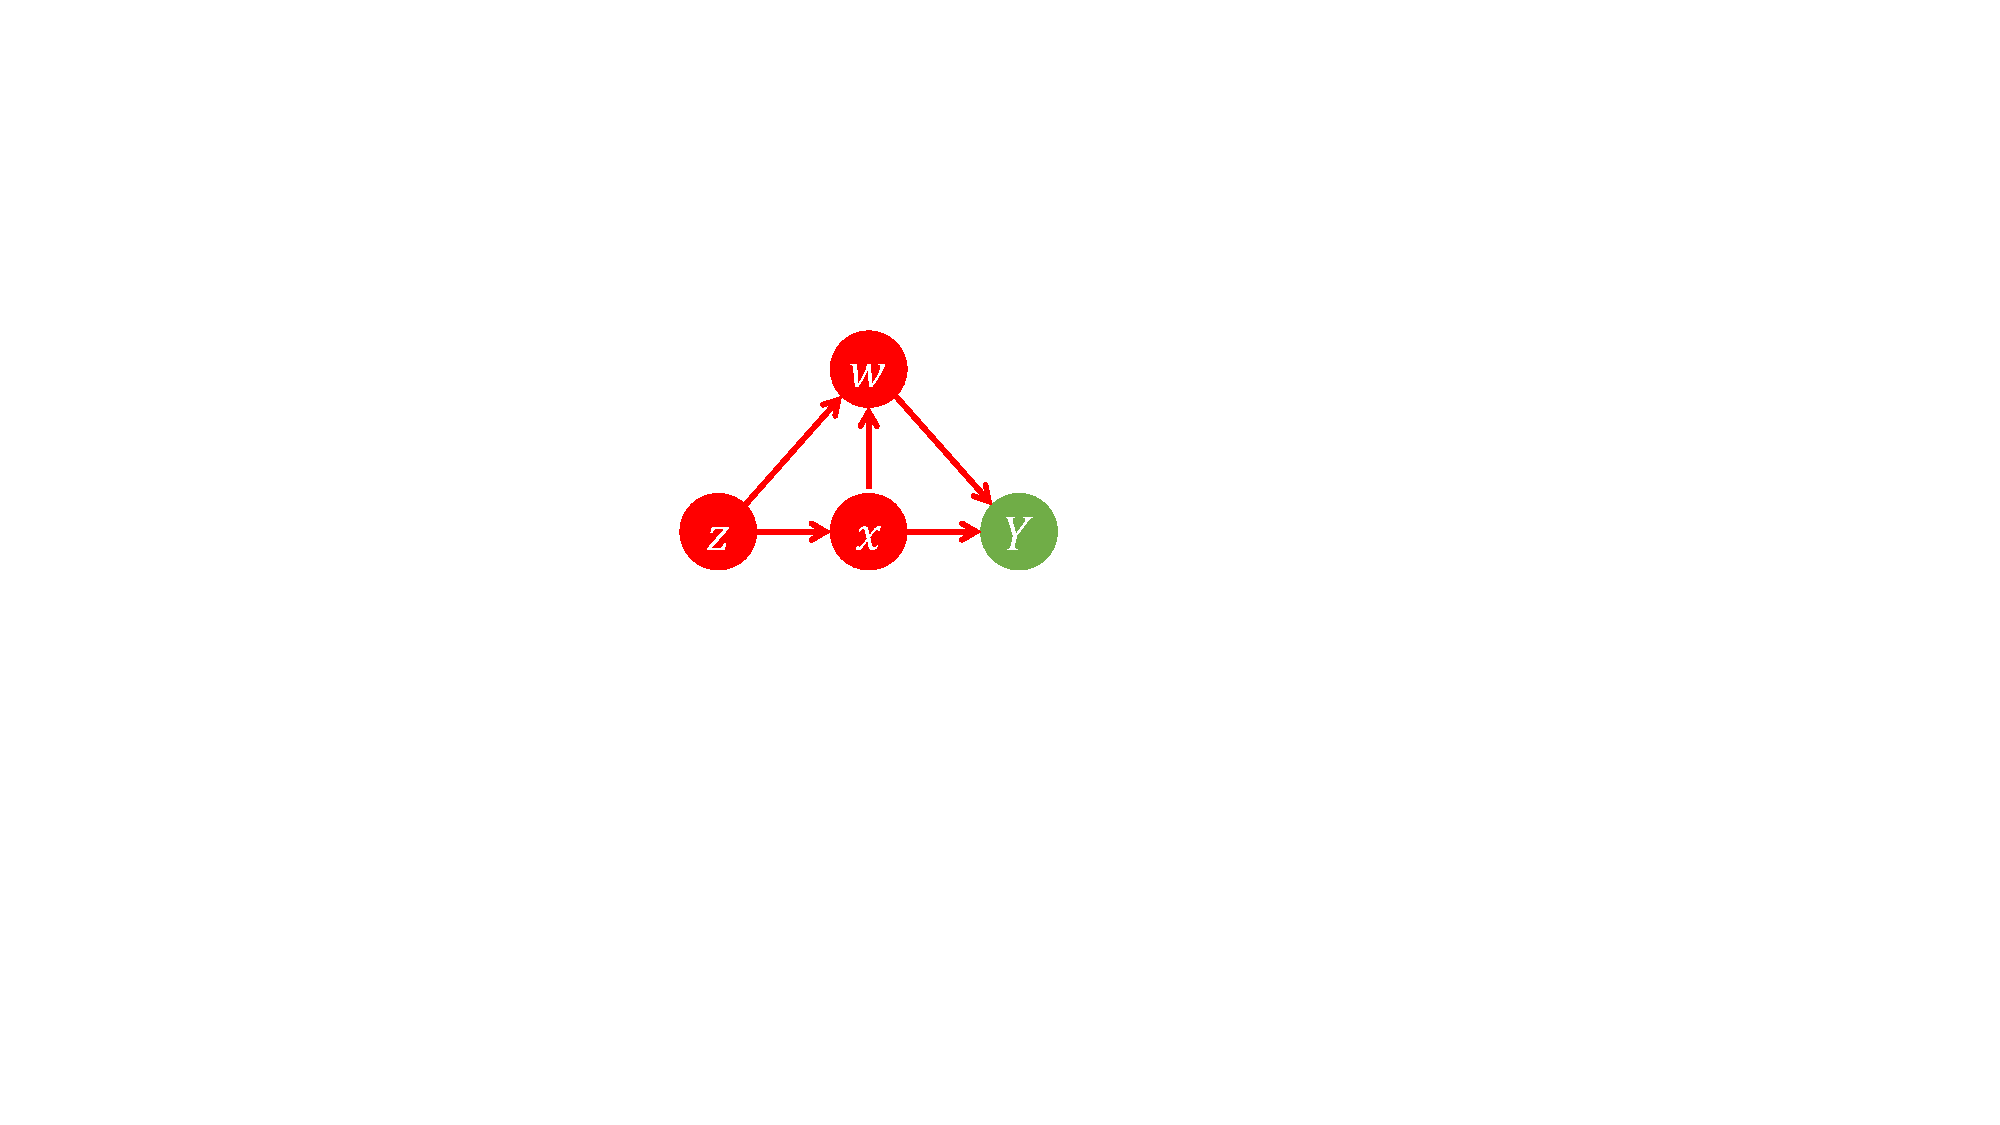
\includegraphics[width=0.25\paperwidth]{conditional_instrument1.pdf}
  %
  \caption{\citep{brito2002generalized} Example without unconditional instruments.}
  %
  \label{fig:conditional_instrument1}
  %
\end{figure}

\citet{pearl2009causality} defines instruments in terms of the conditional distribution in order to increase the probability of finding a valid instrument, especially when unconditional instruments are hard to find. In the Figure~\ref{fig:conditional_instrument1} example, due to existence of $\mathbf{w}$, $\mathbf{z}$ can still cause $\mathbf{y}$ even if we remove $\mathbf{x} \rightarrow Y$, violating \textbf{G2} of Definition~\ref{def:instrument_variable}. In this graph there is no unconditional instrument for $\mathbf{x}$. However, if we hold $\mathbf{w}$ constant, the graph will degenerate to Figure~\ref{fig:conditional_instrument2}
%
\begin{figure}[H]
  %
  \centering
  %
  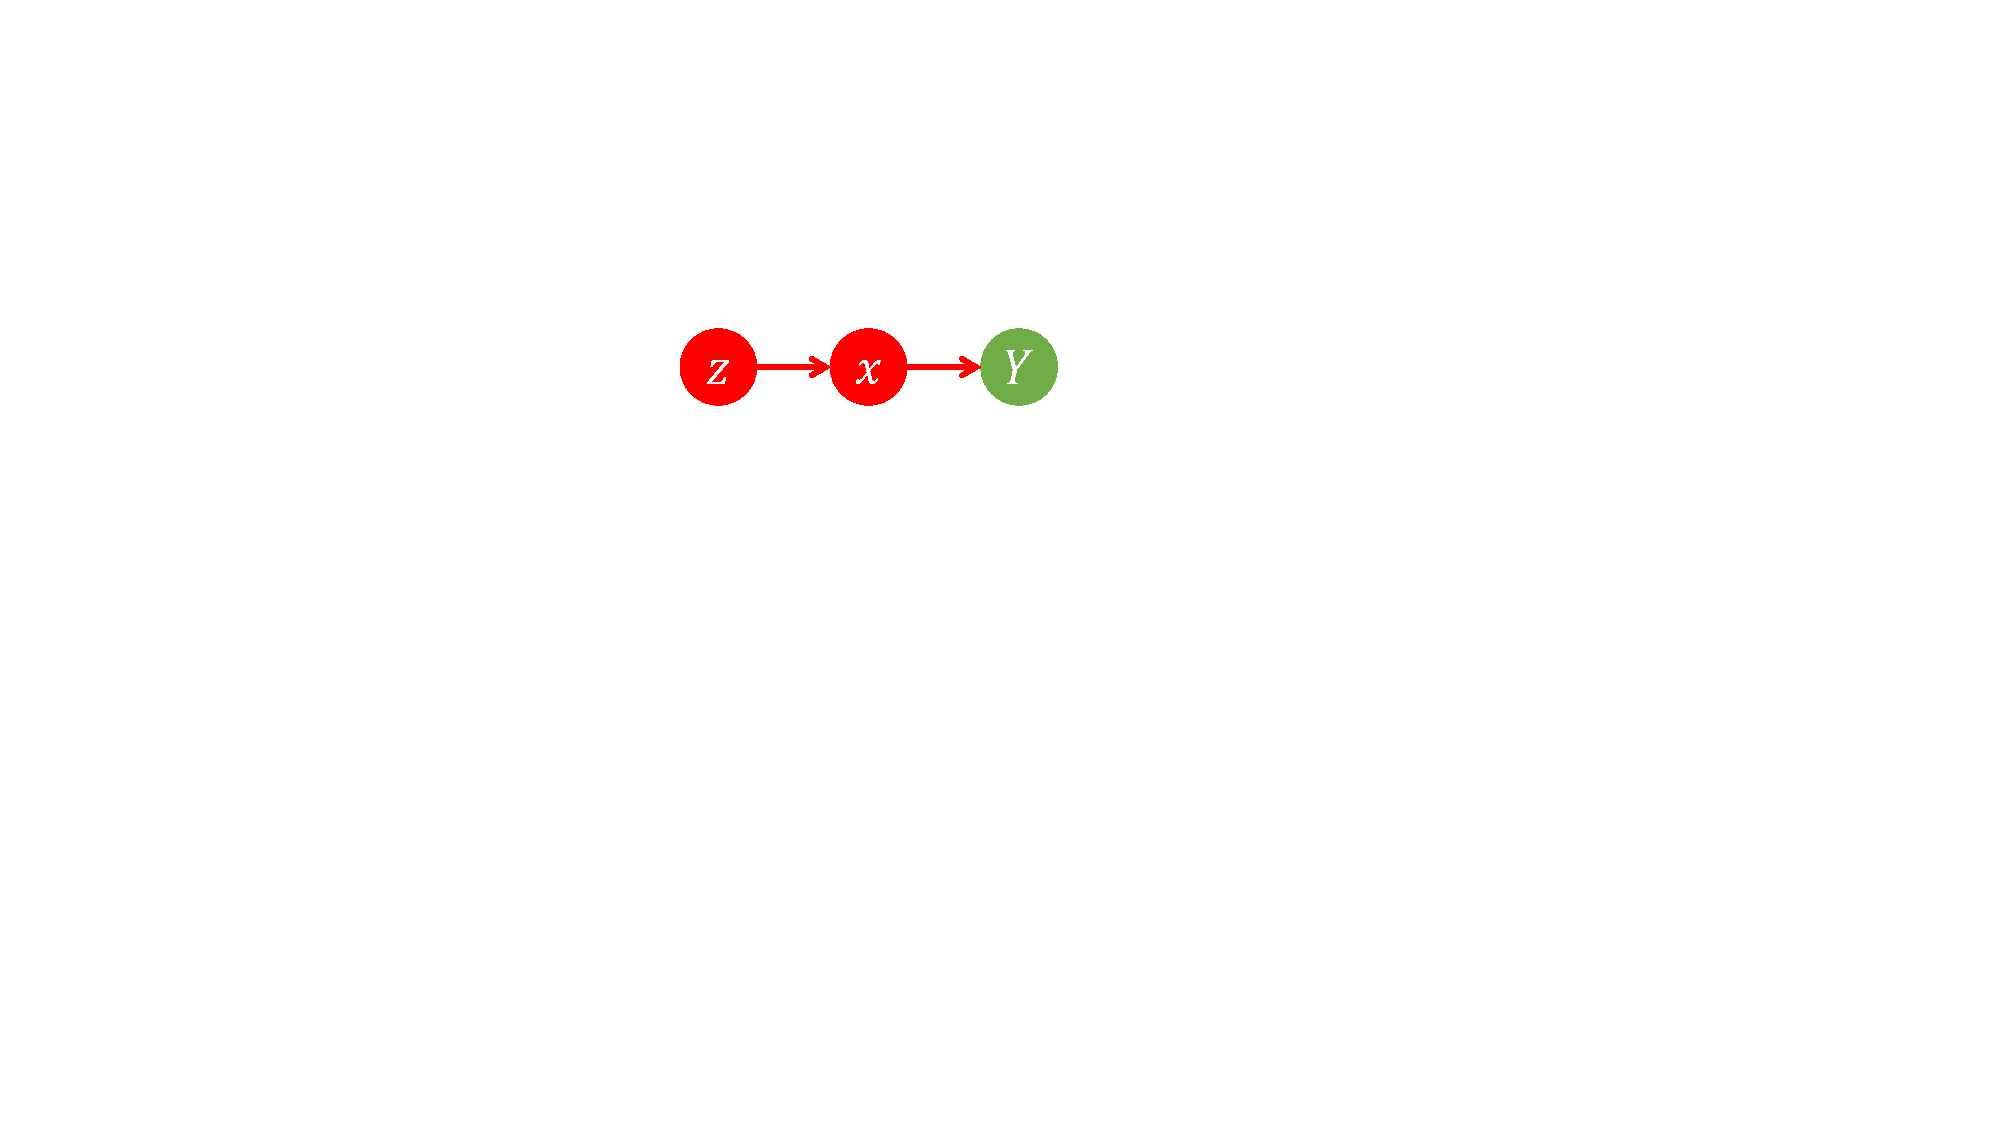
\includegraphics[width=0.25\paperwidth]{Example3_pg.pdf}
  %
  \caption{\citep{brito2002generalized} Controlling for $\mathbf{w}$ in Figure~\ref{fig:conditional_instrument1}, $\mathbf{z}$ is a valid conditional instrument.}
  %
  \label{fig:conditional_instrument2}
  %
\end{figure}
%
\noindent
and $\mathbf{z}$ does not violate \textbf{G1} (that no variable can d-separate $\mathbf{z}$ and $\mathbf{x}$) or \textbf{G2} (that any variable can d-separate $\mathbf{z}$ and $\mathbf{y}$ after removing $\mathbf{x} \rightarrow Y$), implying that $\mathbf{z}$ is a valid conditional instrument for $\mathbf{x}$.

%%%%%%%%%%%%%%%%%%%%%%%%%%%%%%%%%%
%%%%%%%%%%% example %%%%%%%%%%%%%%
%%%%%%%%%%%%%%%%%%%%%%%%%%%%%%%%%%

\subsection*{Graphical examples of instruments}

Next we illustrate that, given an accurately estimated graph, graphical criteria can conveniently  identify invalid instruments.

\subsubsection*{Descendants of $\mathbf{y}$ are invalid instruments for $\mathbf{x}$}

\begin{figure}[H]
	%
	\centering
	%
	\subfloat[\label{fig:not_instrument2a}]
	{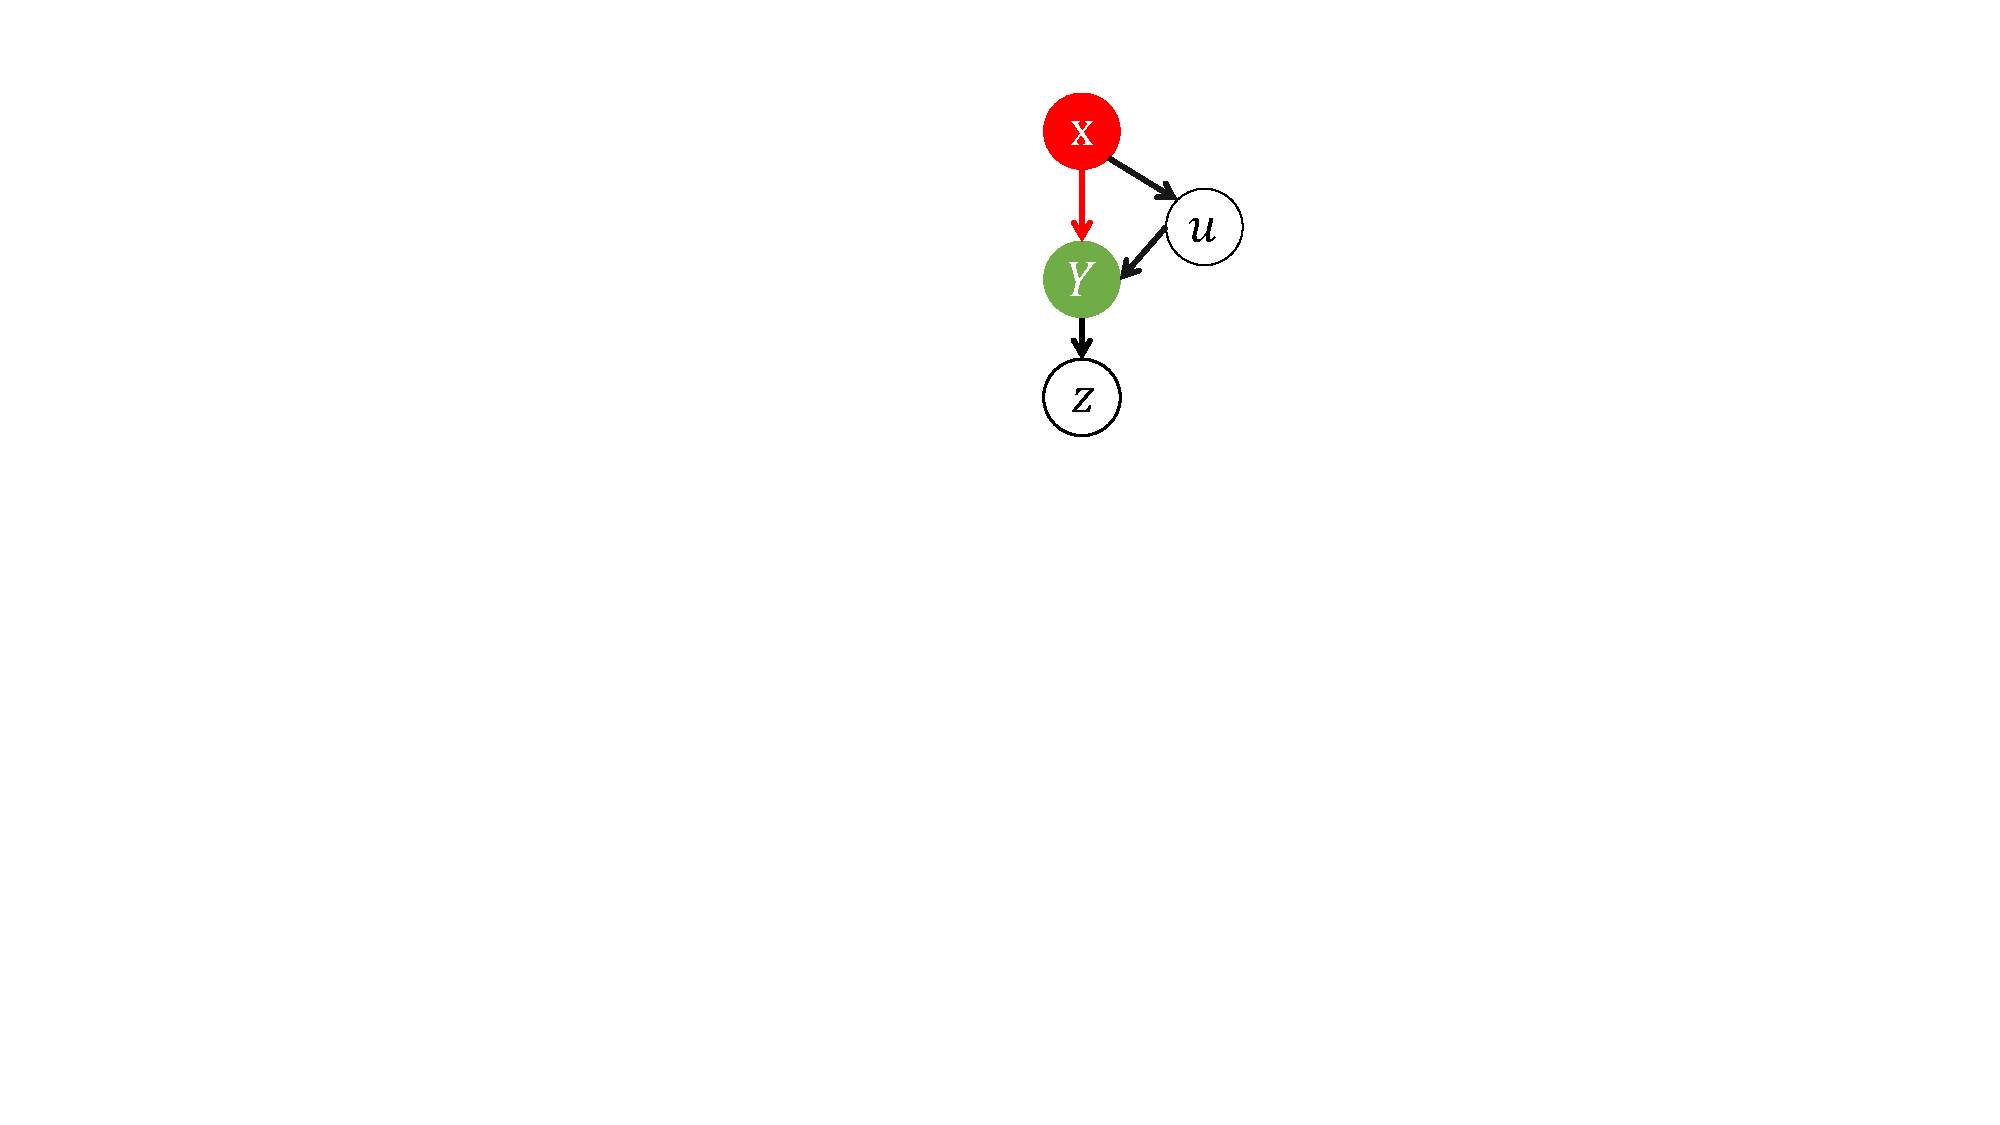
\includegraphics[width=0.1\paperwidth]{not_instrument2.pdf}}
	%
	\hfil
	%
	\subfloat[\label{fig:not_instrument2b}]
	{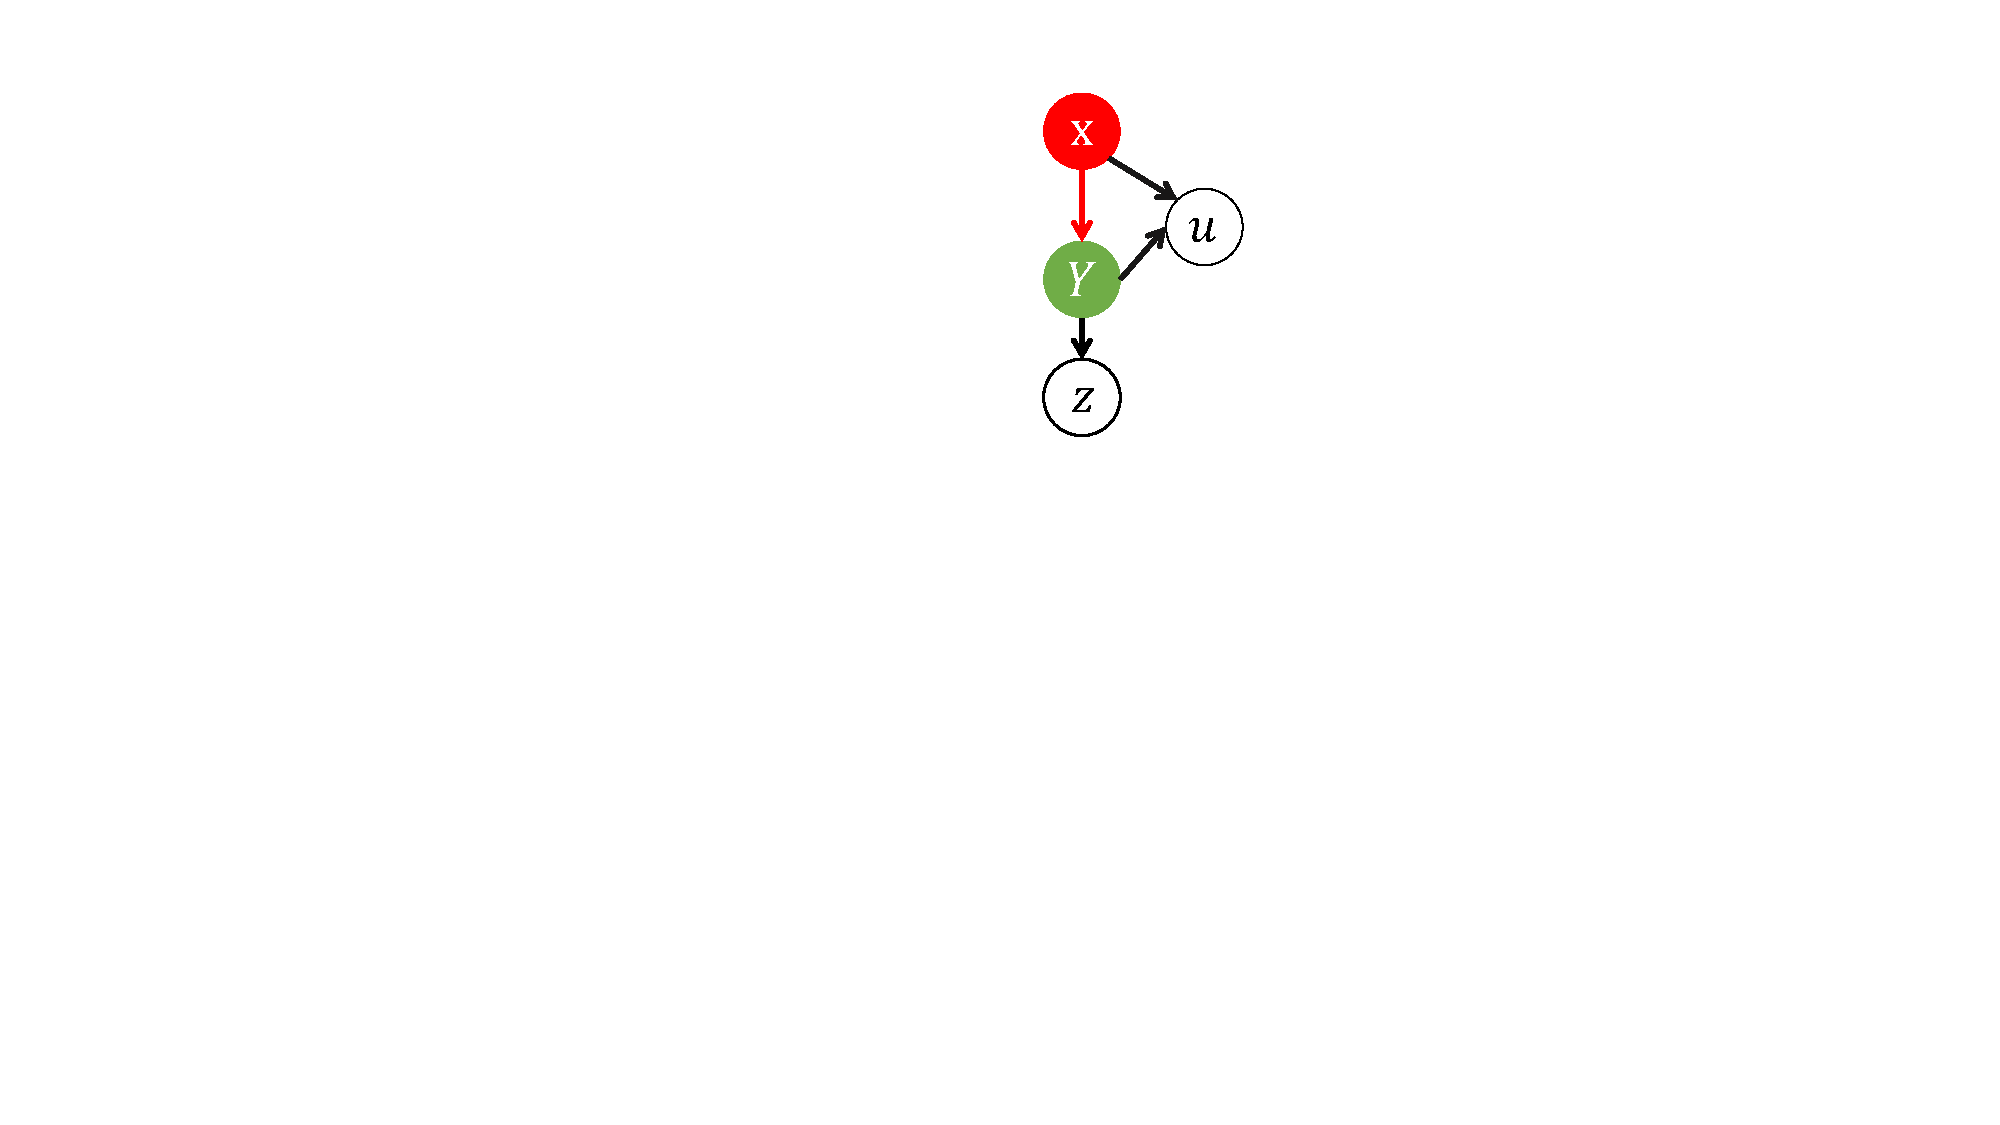
\includegraphics[width=0.1\paperwidth]{not_instrument33.pdf}}
	%
	\hfil
	%
	\subfloat[\label{fig:not_instrument2c}]
	{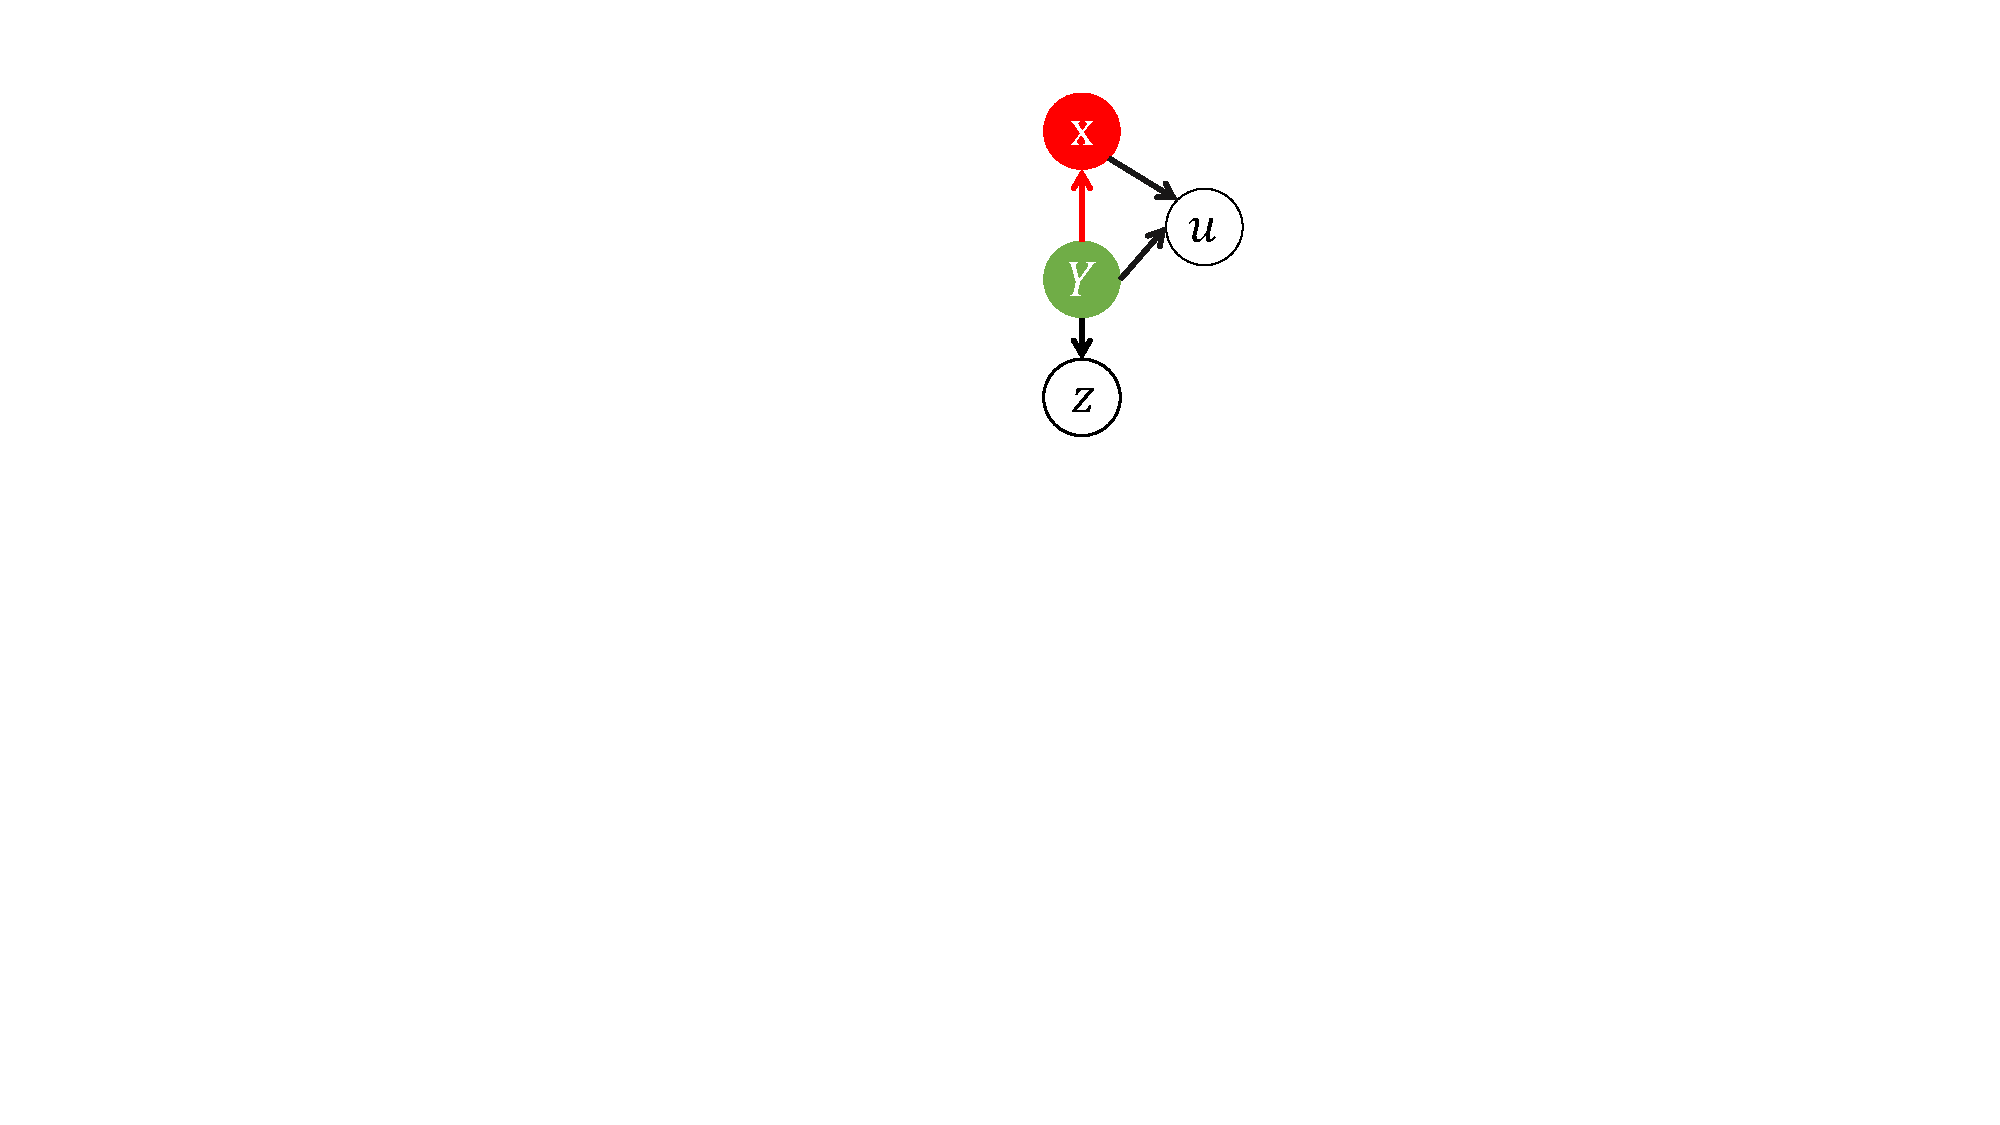
\includegraphics[width=0.1\paperwidth]{not_instrument333.pdf}}
	%
	\hfil
	%
	\subfloat[\label{fig:not_instrument2d}]
	{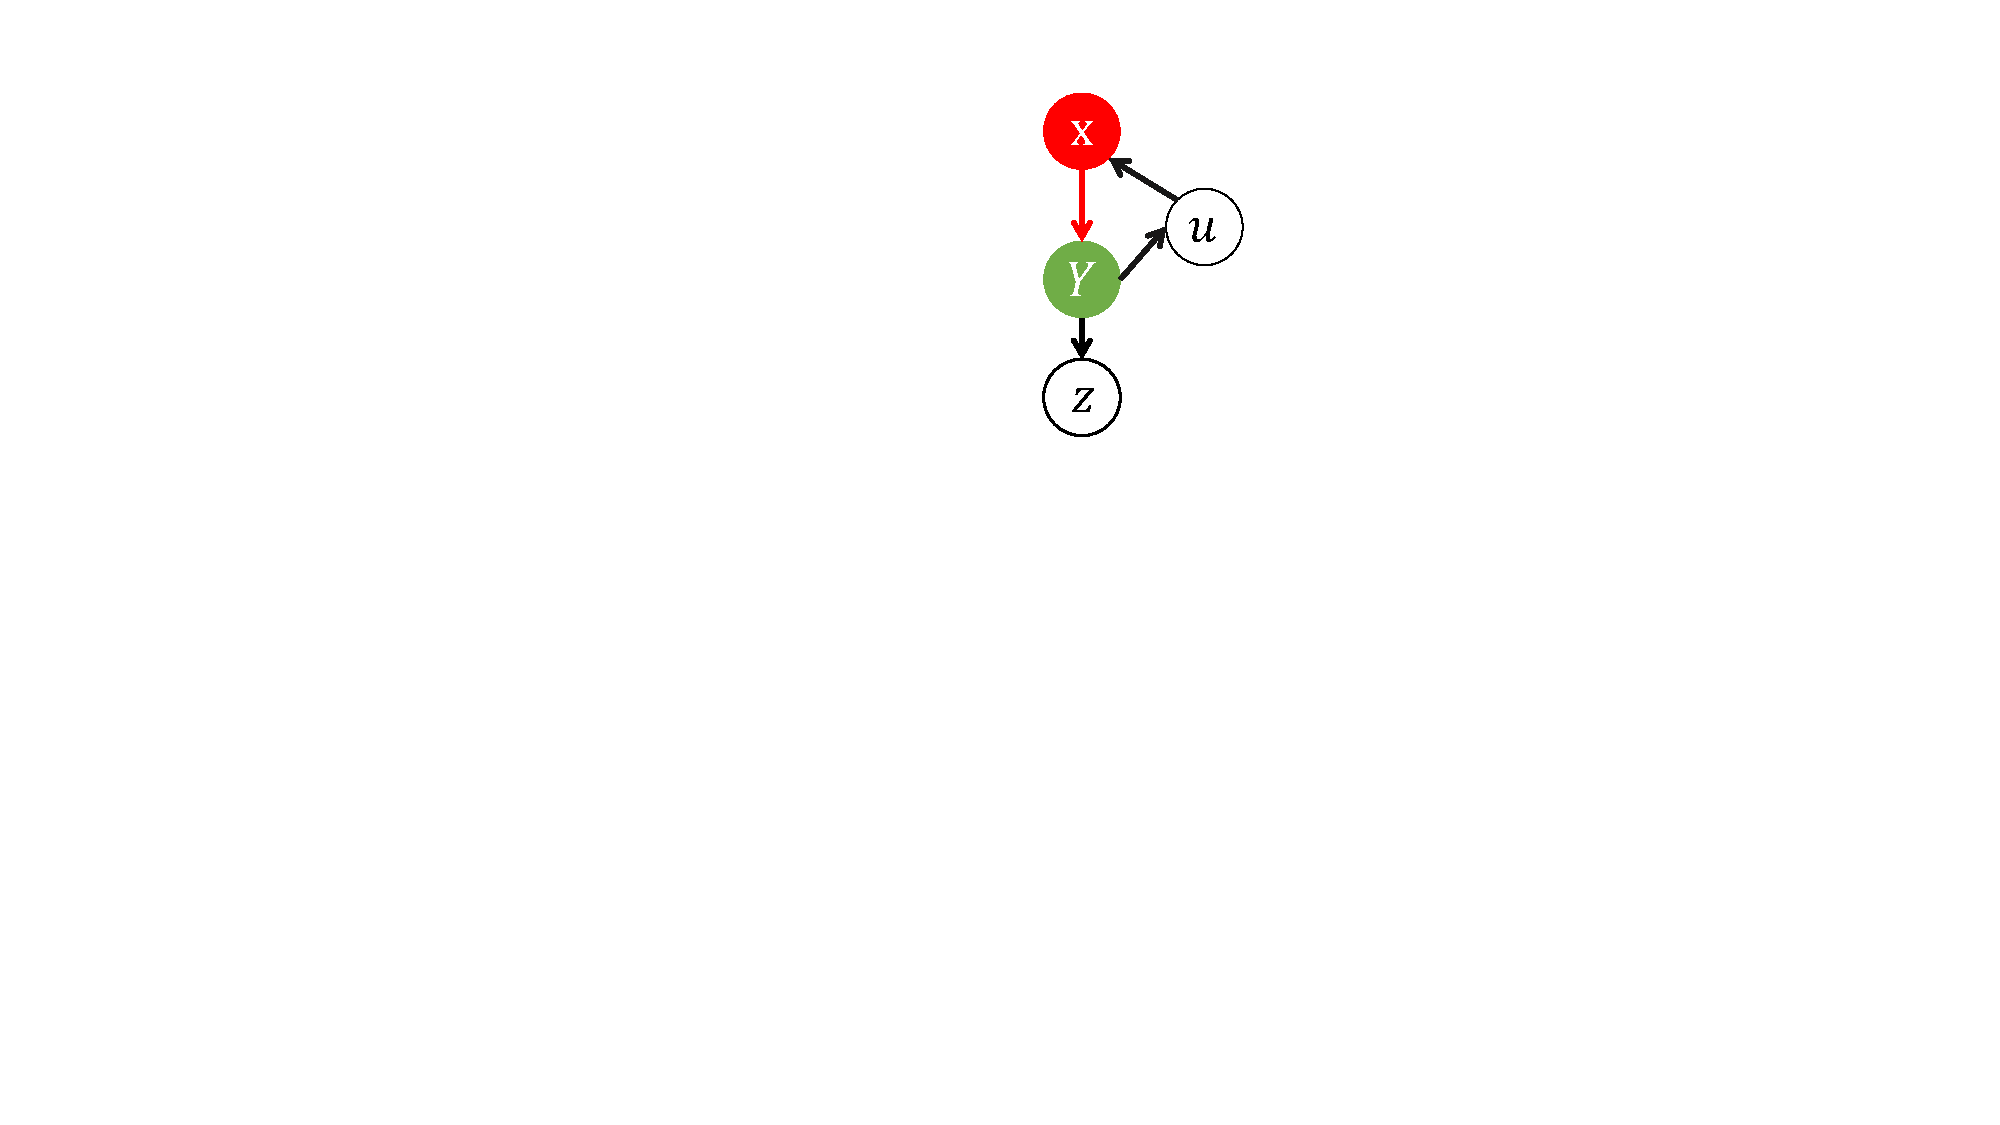
\includegraphics[width=0.1\paperwidth]{not_instrument3333.pdf}}
	%
	\caption{$\mathbf{z}$ (descendant of $\mathbf{y}$) cannot be a valid instrument.}
	\label{fig:not_instrument2}
	%
\end{figure}

Figure~\ref{fig:not_instrument2} explains why descendants of $\mathbf{y}$ cannot be instruments. In all 4 figures, $\mathbf{z}$ is the child of $\mathbf{y}$, meaning that $\mathbf{z} \not\ind Y$ for any variable in $G_{\overline{X}}$. This implies that the effect from $\mathbf{z}$ to $\mathbf{y}$ does not go through $\mathbf{x}$ at all. Thus, G1 in Definition~\ref{def:instrument_variable} is violated in all 4 figures.

Such violations can also be explained using the econometrics definition of an instrument. Regardless of the other arrows, there are only two possible relations among $\mathbf{z}$, $\mathbf{y}$ and $u$: either $u \rightarrow Y \rightarrow \mathbf{z}$ or $u \leftarrow Y \rightarrow \mathbf{z}$.\footnote{Because we assume $\mathbf{z}$ is a descendant of $\mathbf{y}$, $Y \rightarrow \mathbf{z}$ always.} If $u \rightarrow Y \rightarrow \mathbf{z}$ (as in Figure~\ref{fig:not_instrument2a}), $\mathrm{corr} \left( \mathbf{z}, u \right) \neq 0$. If $u \leftarrow Y \rightarrow \mathbf{z}$ (as in Figures~\ref{fig:not_instrument2b} to \ref{fig:not_instrument2d}), $\mathbf{y}$ confounds $\mathbf{z}$ and $u$, implying that the unconditional correlation $\mathrm{corr} \left( \mathbf{z}, u \right)$ is also nonzero. Thus, $\mathrm{corr} \left( \mathbf{z}, u \right)=0$ only if both $\mathbf{z}$ and $u$ are ancestors of $\mathbf{y}$.

\subsubsection*{Descendants of $\mathbf{x}$ are invalid instruments for $\mathbf{x}$}

Using descendants of $\mathrm{x}$ as instruments will inevitably violate the econometrics definition of an instrument. Regardless of the other arrows in Figure~\ref{fig:not_instrument3}, there are only two possible scenarios relating $\mathbf{z}$, $\mathbf{x}$ and $u$: either $u \rightarrow \mathbf{x} \rightarrow \mathbf{z}$ or $u \leftarrow \mathbf{x} \rightarrow \mathbf{z}$.\footnote{Because we assume $\mathbf{z}$ is a descendant of $\mathbf{x}$, $\mathbf{x} \rightarrow \mathbf{z}$ always.}

\begin{figure}[H]
	%
	\centering
	%
	\subfloat[\label{fig:not_instrument3a}]
	{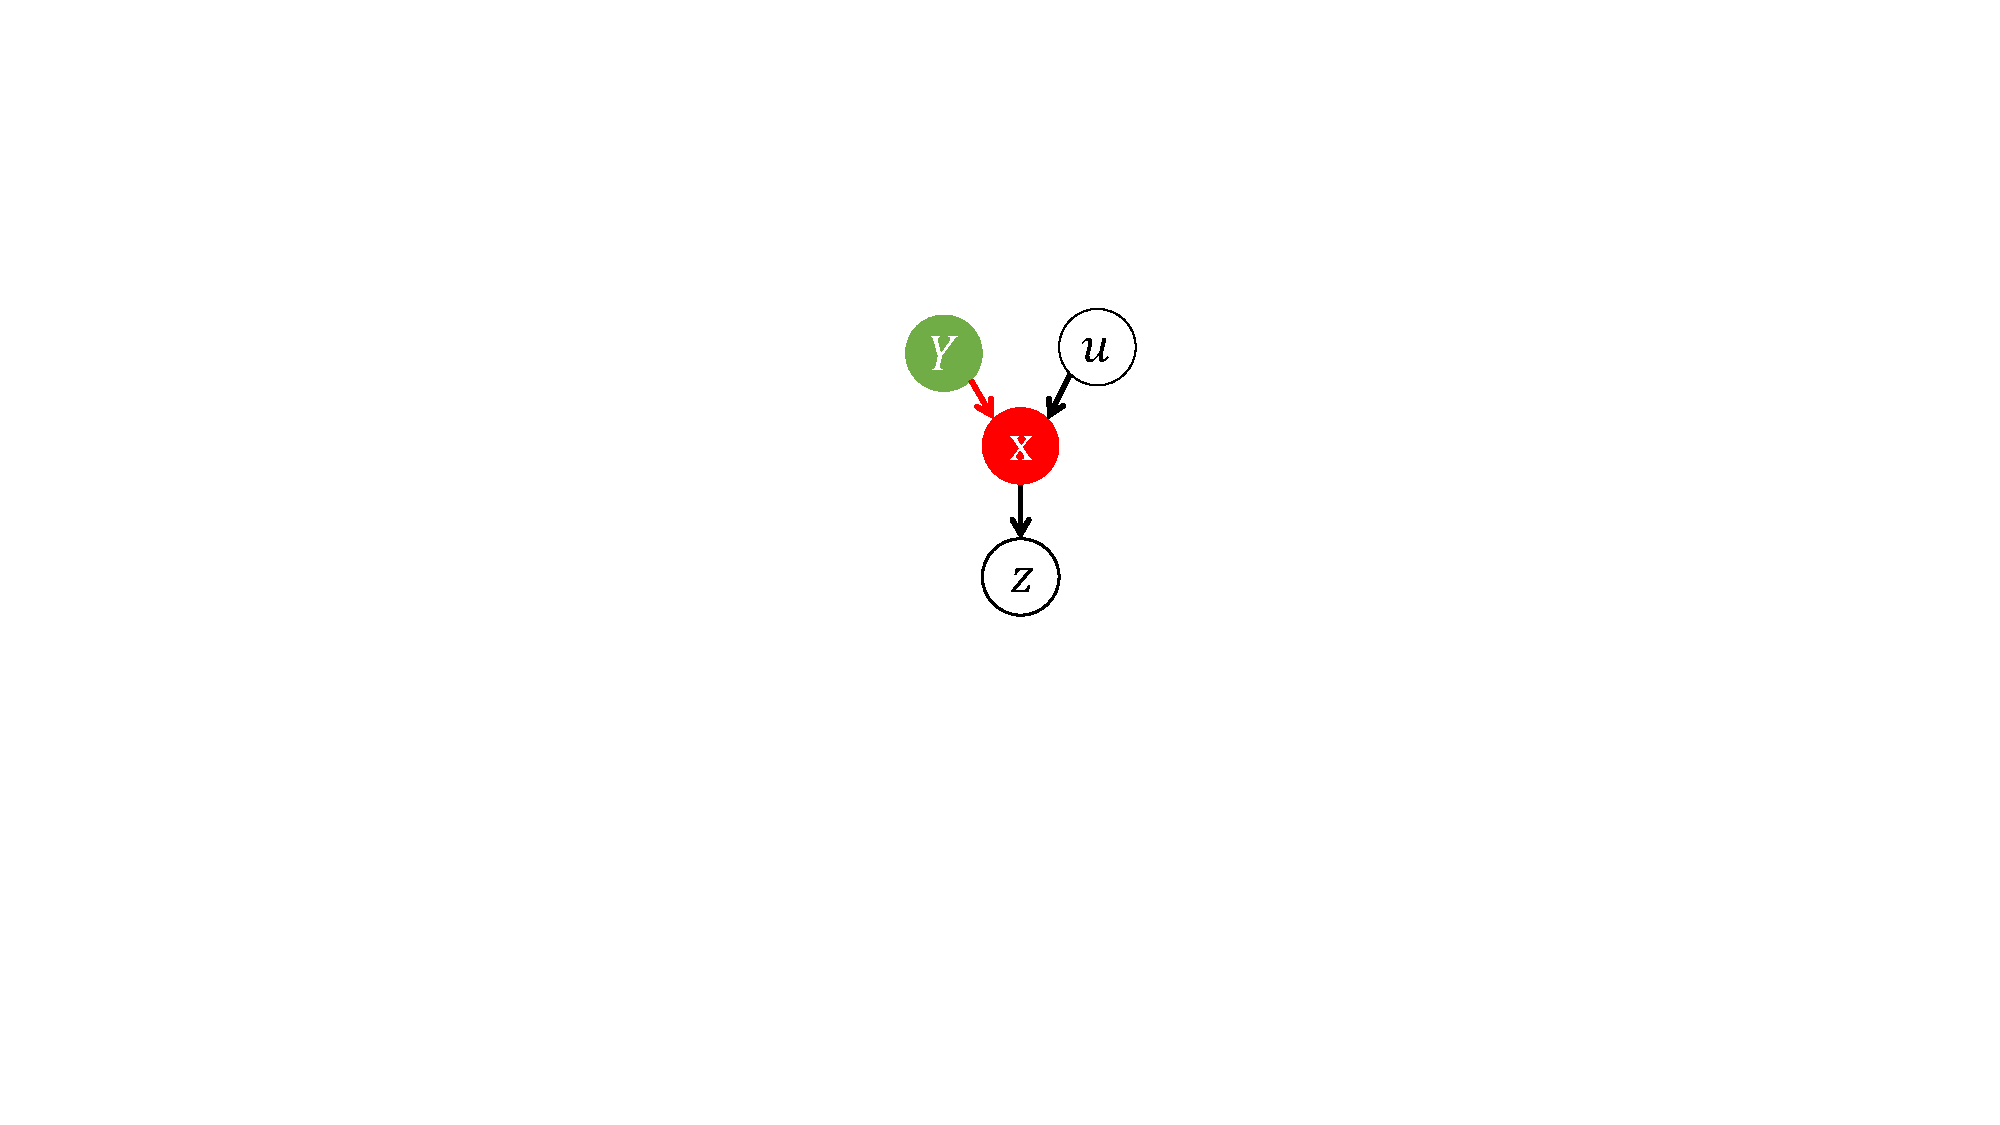
\includegraphics[width=0.13\paperwidth]{not_instrument3.pdf}}
	\hfil
	\subfloat[\label{fig:not_instrument3b}]
	{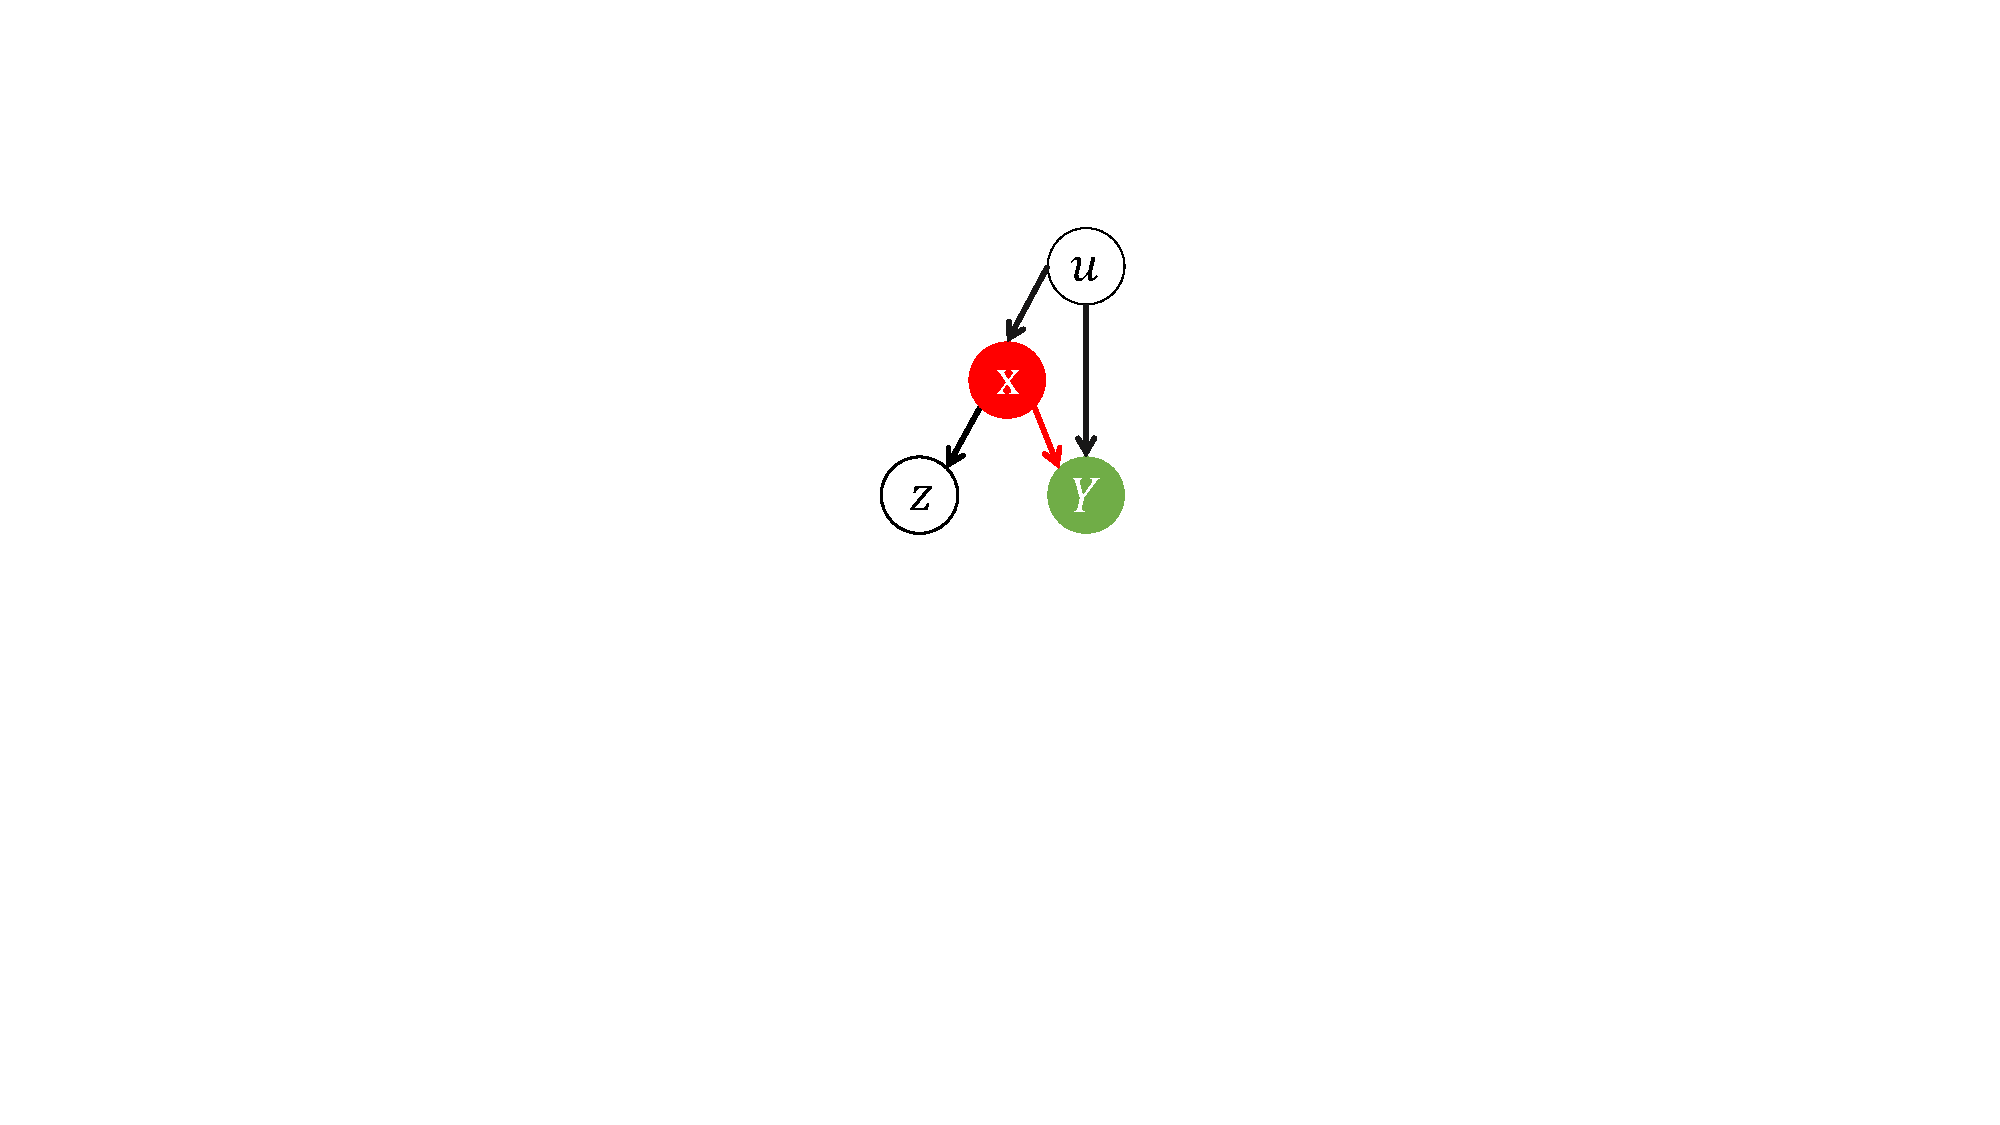
\includegraphics[width=0.12\paperwidth]{not_instrument5.pdf}}
	\hfil
	\subfloat[\label{fig:not_instrument3c}]
	{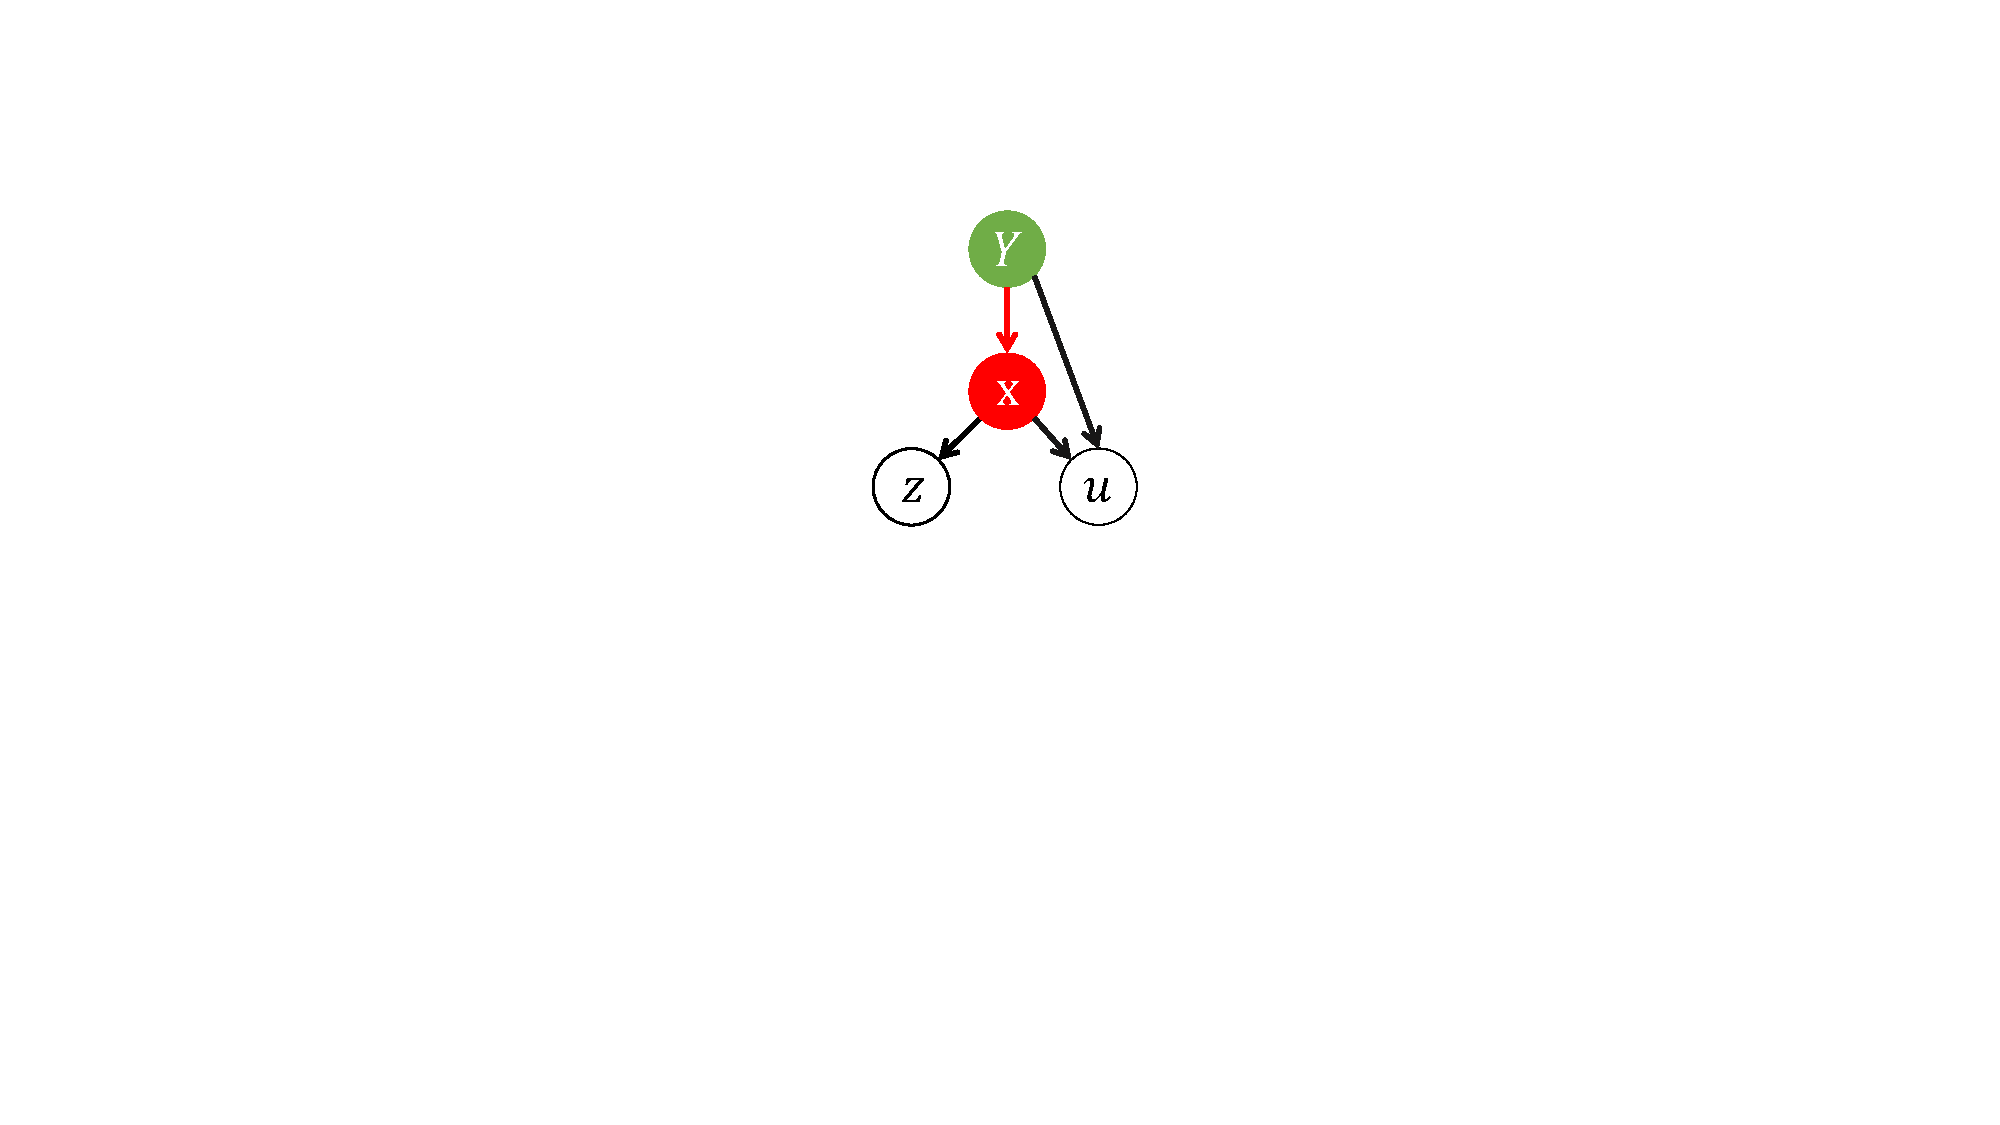
\includegraphics[width=0.13\paperwidth]{not_instrument6.pdf}}
	\hfil
	\subfloat[\label{fig:not_instrument3d}]
	{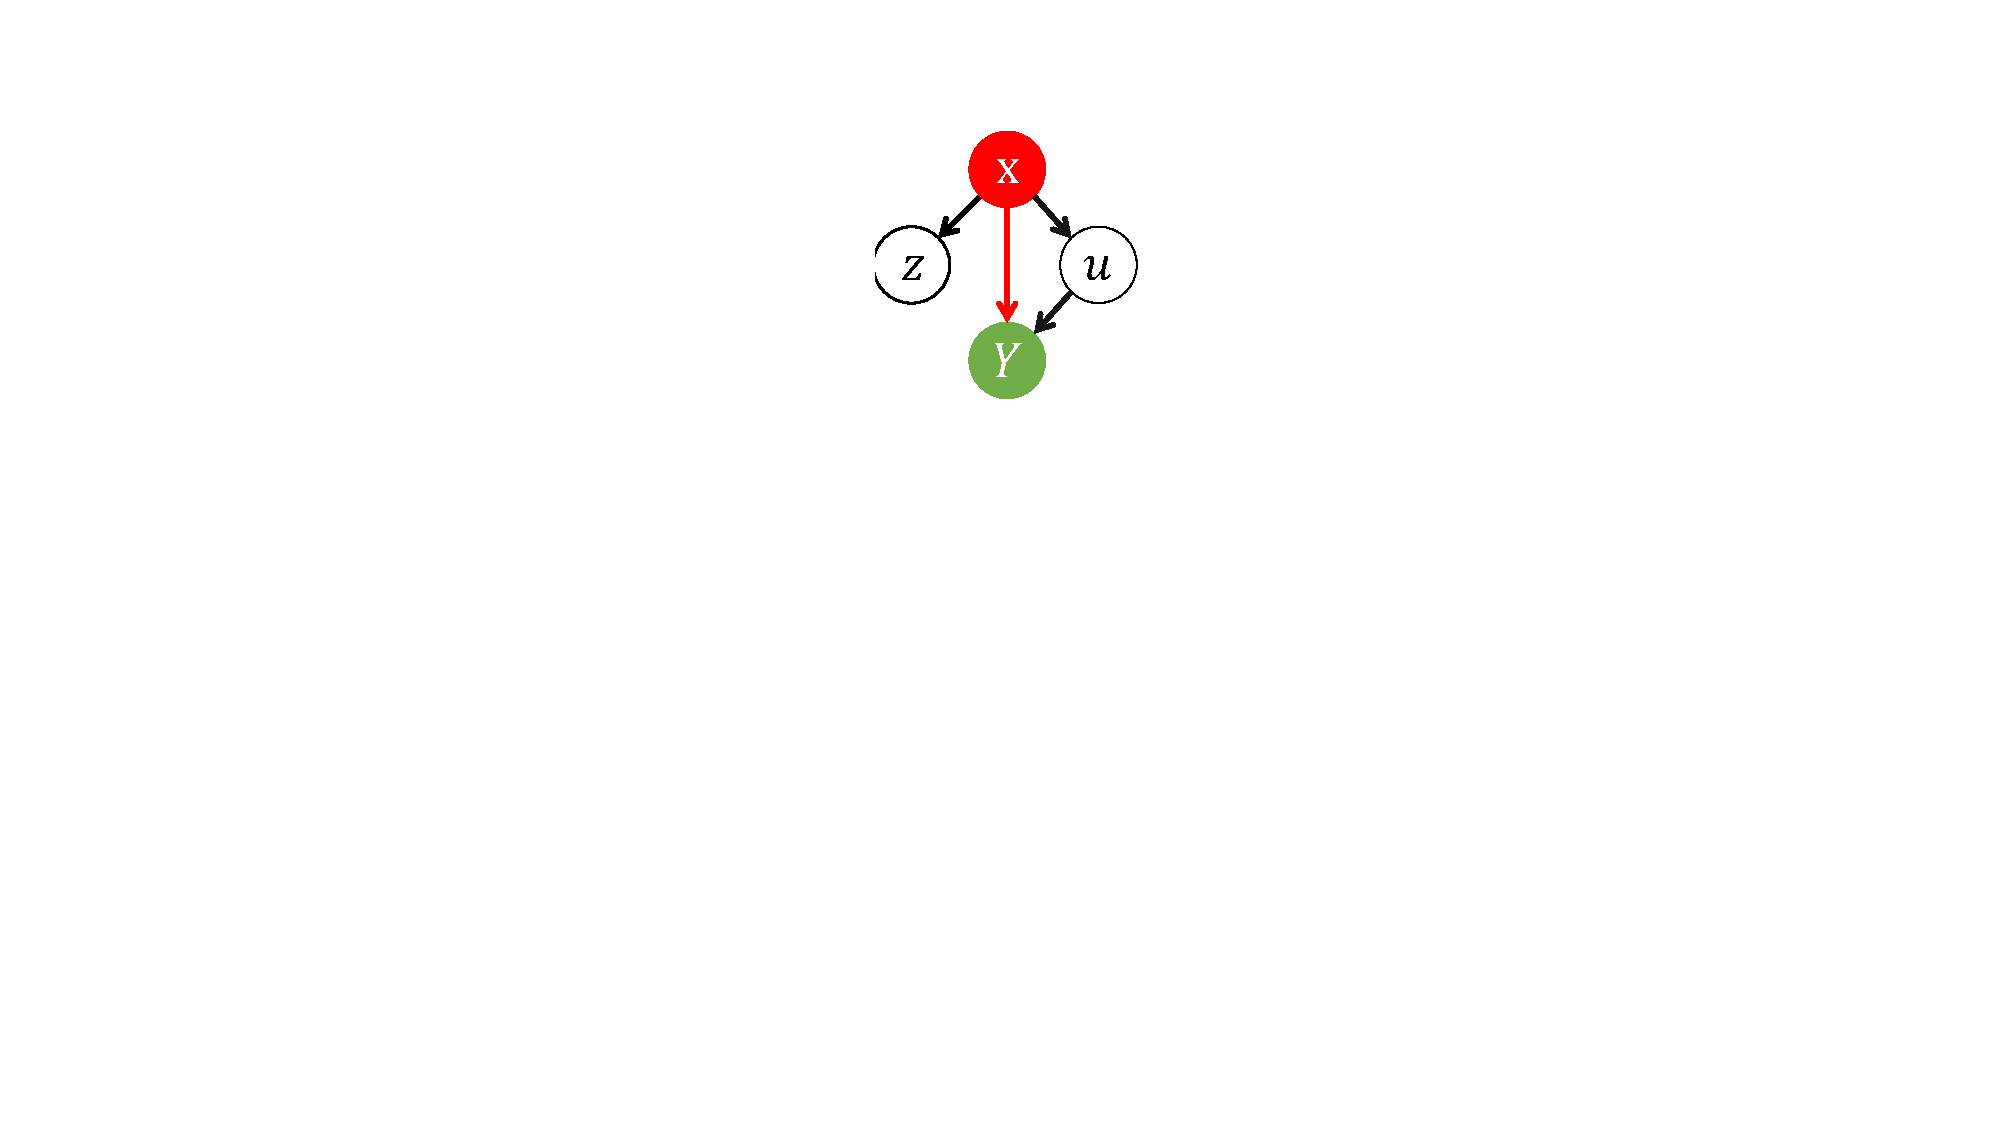
\includegraphics[width=0.13\paperwidth]{not_instrument4.pdf}}
	%
	\caption{Illustration: violation of Definition~\ref{def:instrument_variable}.}
	\label{fig:not_instrument3}
	%
\end{figure}

If $u \rightarrow \mathbf{x} \rightarrow \mathbf{z}$ (as in Figures~\ref{fig:not_instrument3a} and \ref{fig:not_instrument3b}), $\mathrm{corr} \left( \mathbf{z}, u \right) \neq 0$. If $u \leftarrow \mathbf{x} \rightarrow \mathbf{z}$ (as in Figures~\ref{fig:not_instrument3c} to \ref{fig:not_instrument3d}), $\mathbf{x}$ confounds $\mathbf{z}$ and $u$, implying the marginal correlation $\mathrm{corr} \left( \mathbf{z}, u \right)$ is also nonzero. As a result, $\mathrm{corr} \left( \mathbf{z}, u \right) = 0$ only when both $u$ and $\mathbf{z}$ are the ancestors of $\mathbf{x}$.

Equivalently, using descendants of $\mathrm{x}$ as instruments will violate Definition~\ref{def:instrument_variable}. In the case $u \rightarrow \mathbf{x} \rightarrow \mathbf{z}$, if $\mathbf{y}$ is also the ancestor of $\mathbf{x}$ (as in Figures~\ref{fig:not_instrument3a} and \ref{fig:not_instrument3c}), Definition~\ref{def:instrument_variable} will be violated since $\mathbf{x} \rightarrow Y$ does not exist at all. If $\mathbf{y}$ is also a descendant of $\mathbf{x}$ (as in Figures~\ref{fig:not_instrument3b} and \ref{fig:not_instrument3d}), $\mathrm{x}$ confounds both $\mathrm{z}$ and $\mathbf{y}$, implying that the unconditional correlation between $\mathbf{z}$ and $\mathbf{y}$ is nonzero in $G_{\overline{X}}$. Hence, $\mathbf{z} \not\ind Y$ for $u$ in $G_{\overline{X}}$, which violates G1 in Definition~\ref{def:instrument_variable}.

\subsubsection*{Remote ancestors of $\mathbf{x}$ and $\mathbf{y}$ are highly likely to be weak instruments for $\mathbf{x}$}

As explained earlier, ancestors of $\mathbf{x}$ and $\mathbf{y}$ are more likely to satisfy both the graphical- and error-based criteria. However, close ancestors are preferred when choosing the instruments. The more remote the ancestors of $\mathbf{x}$ and $\mathbf{y}$, the weaker are their correlations to $\mathbf{x}$ and $\mathbf{y}$. If all variables are standardized, in 2SLS
%
\[
  %
  b_{IV} = \frac{\mathrm{corr} \left(\mathbf{z}, Y\right)}{\mathrm{corr} \left(\mathbf{z}, \mathbf{x}\right)}.
  %
\]
%
Thus, remote ancestors are more likely to be weak instruments and to cause bias.

\newpage
%\section*{References}%%%%%%%%%%%%%%%%%%%%%%%%%%%%%%%%%%%%%%%%%%%%%%%%%%%%%%%%%%%%%%%%%%%%%%%%%%%%%%

%\bibliographystyle{elsarticle-harv}
%\bibliographystyle{CJE}

%\bibliography{CVrefs}

\end{document}

%%%%%%%%%%%%%%%%%%%%%%%%%%%%%%%%%%
%%%%%%%%%%%%%%%%%%%%%%%%%%%%%%%%%%
%%%%%%%%%%%%%%%%%%%%%%%%%%%%%%%%%%
